% arara: pdflatex
\documentclass[headings=small,a4paper,11pt,oneside]{scrreprt}

\setcounter{tocdepth}{3}
\setcounter{secnumdepth}{3}

\usepackage{setspace}
\usepackage[right=4cm,top=3cm,left=2cm,bottom=3cm]{geometry}
\usepackage[utf8]{inputenc}
\usepackage[ngerman]{babel}
\usepackage[T1]{fontenc}
\usepackage{lmodern}
\usepackage{scrlayer-scrpage}
\usepackage{blindtext}
\usepackage{graphicx}
\usepackage[hyphens]{url}
\usepackage{hyperref}
\usepackage{caption}
\usepackage{tabularx}
\usepackage{graphicx}
\makeatletter
\def\ScaleIfNeeded{%
\ifdim\Gin@nat@width>\linewidth
\linewidth
\else
\Gin@nat@width
\fi
}
\makeatother
\usepackage[font={small},%
  labelsep=space]{caption}
\newcolumntype{L}[1]{>{\raggedright\arraybackslash}p{#1}}
\newcolumntype{C}[1]{>{\centering\arraybackslash}p{#1}}
\newcolumntype{R}[1]{>{\raggedleft\arraybackslash}p{#1}}

\graphicspath{ {./images/} }

\automark{chapter}
\automark*{section}
\clearpairofpagestyles
\ihead{\headmark}
\ohead{\pagemark}

\renewcommand*{\chapterpagestyle}{empty}

\renewcommand{\autodot}{}% Remove all end-of-counter dots

\renewcommand*\chapterheadstartvskip{\vspace*{-\topskip}}
\renewcommand*\chapterheadendvskip{%
  \vspace*{1\baselineskip plus .1\baselineskip minus .167\baselineskip}}

\begin{document}

\newgeometry{right=2cm,top=2cm,left=2cm,bottom=2cm}
\singlespacing
\titlehead{Humboldt-Universität zu Berlin\\
Philosophische Fakultät\\
Institut für Geschichtswissenschaften\vspace*{4cm}}
\subject{Masterarbeit}
\title{Open Science in den Geschichtswissenschaften?}
\subtitle{Konzeption eines offenen Forschungsdatenmanagements am Beispiel von Forschungsdaten zur Vernichtung der jüdischen Gewerbetätigkeit im Nationalsozialismus}
\author{vorgelegt von:\\Sophie Eckenstaler}
\date{am 07.06.2022\vspace*{3.7cm}}
\publishers{\normalsize
%Layout für markdown-Generierung
Erstbetreuer: Prof. Dr. Rüdiger Hohls, Institut für Geschichtswissenschaften, HU Berlin\\ 
Zweitbetreuer: Prof. Dr. Michael Wildt, Institut für Geschichtswissenschaften, HU Berlin\\
Studiengang: Master of Arts, Geschichtswissenschaften, Schwerpunkt: Digital History\\
Matrikelnr.: 596272\\
E-Mail: sophie.eckenstaler@hu-berlin.de\\
Eberswalde, den 7. Juni 2022
% Layout für den Druck auskommentieren
%\raggedright
%\begin{tabbing}
%\hspace{1.2in}\=\hspace{1in}\=\kill
%Erstbetreuer:\>Prof. Dr. Rüdiger Hohls, Institut für Geschichtswissenschaften, HU Berlin\\ 
%Zweitbetreuer:\>Prof. Dr. Michael Wildt, Institut für Geschichtswissenschaften, HU Berlin\\
%Studiengang:\>Master of Arts, Geschichtswissenschaften, Schwerpunkt: Digital History\\
%Matrikelnr.:\>596272\\
%E-Mail:\>sophie.eckenstaler@hu-berlin.de\\
%\end{tabbing}
}



\maketitle

\singlespacing
\tableofcontents
\restoregeometry

\singlespacing
\chapter{Einleitung}
\onehalfspacing

\section{Motivation}

Im Zusammenhang mit der COVID-19-Pandemie erlebt Open Science seit 2020 enormen Aufschwung in der Wissenschaft. Deren Kerneigenschaften des ungehinderten kollaborativen Austauschs von Daten, Papers und Zwischenergebnissen werden eine entscheidende Rolle bei der raschen Impfstoffentwicklung zugewiesen. Vielfach wurde und wird daher die Bedeutung und Wirkung von Open Science gegenwärtig insbesondere im medizinischen und naturwissenschaftlichen Wissenschaftsbereich diskutiert.\footnote{Siehe zum Beispiel Lonni Besançon, Nathan Peiffer-Smadja, Corentin Segalas, Haiting Jiang, Paola Masuzzo, Cooper Smout, Eric Billy, Maxime Deforet, Clémence Leyrat: Open science saves lives: lessons from the COVID-19 pandemic, in: BMC Medical Research Methodology, Band 21, Artikelnr. 117, 2021, doi:10.1186/s12874-021-01304-y und CODATA Coordinated Expert Group (2020): Open Science for a Global Transformation. CODATA coordinated submission to the UNESCO Open Science Consultation, Zenodo, doi:10.5281/zenodo.3935461.} Die große Zahl an Open Science Initiativen zeigt zudem, dass Open Science in der Wissenschaft angekommen und in Begriff ist, sich dort zu etablieren. Im Kern geht es auch darum, die Integrität von wissenschaftlicher Forschung zu wahren, sie gerade im sogenannten postfaktischen Zeitalter zu stärken und sie somit weniger anfällig für Betrug und Fälschung in einer digitalen Welt zu machen.Auch auf gesellschaftspolitischer Ebene gewinnt Open Science an Relevanz. Die Europäische Union hat Open Science zu einem von insgesamt drei Grundsatzzielen für die Forschungsarbeit in Europa erklärt und die Deutsche UNESCO-Kommission hebt in ihrer Empfehlung von 2020 deren gesellschaftliche Bedeutung hervor:

\begin{quote}     
    ,,Darüber hinaus besteht mit Open Science eine Chance auf die praktische Umsetzung von seit Langem bestehenden politischen Forderungen: Mit Open Science kann Teilhabe an und Zugang zu wissenschaftlichen Erkenntnissen als Gemeingut und Menschenrecht praktisch umgesetzt werden, wie es bereits seit Ende des Zweiten Weltkriegs in der Allgemeinen Erklärung der Menschenrechte gefordert war.''\footnote{Deutsche UNESCO-Kommission e.V. (Hrsg.): Open Science. Perspektiven aus Deutschland auf die Erarbeitung der geplanten Empfehlung der UNESCO. UNESCO recommendation on Open Science, Berlin 2020, S. 8.}    
\end{quote}

In der Konsequenz stellt sich auch für die Geschichtswissenschaften die Frage, einserseits welche Wirkung Open Science auf die historische Forschung und andererseits welche Wirkung historische Forschung mit Open Science entfalten kann. Hierauf möchte die Arbeit Antworten finden, indem am Beispiel eines geschichtswissenschaftlichen Forschungsfelds die praktische Umsetzung von Open Science untersucht wird. Damit trägt sie zum Anschluss der Geschichtswissenschaften an gegenwärtig aktuelle wissenschaftliche Debatten bei und kann neue Wege in der digitalen Welt für die historische Forschung explorieren. 

\section{Zielsetzung}

Ausgehend von Forschungsdaten zu Jüdischen Gewerbebetrieben soll erstmals überhaupt ein gesamtheitliches Forschungsdatenmanagement für diese entwickelt werden. Der Fokus liegt dabei auf Studien, die systematisch Daten zu Jüdischen Gewerbebetrieben zum Zwecke der Erkenntnisgenerieung gesammelt haben. In das Forschungsdatenmanagement sollen Open Science-Ansätze integriert und im Zuge dessen die Implementierbarkeit sowie der Nutzen für die historische Forschung ausgelotet werden. Ziel ist es, am Ende ein prototypisches Konzept zu offenem Forschungsdatenmanagemet mit Open Science-Bezug vorliegen zu haben, das auch für andere historische Felder insbesondere der Zeitgeschichte übertragbar und nutzbar wäre.

\section{Methodisches Vorgehen}

Bei der Konzeption eines Forschungsdatenmanagements wird sich an etablierte softwaretechnische Verfahren orientiert. Im Kern basiert es auf einer Anforderungsanalyse, wie sie auch im Software-Engineering verwendet wird.\footnote{Siehe zum Beispiel M. Broy, M. Kuhrmann: Anforderungsanalyse und Anforderungsmanagement, in: Einführung in die Softwaretechnik, Berlin, Heidelberg 2021, S. 199-222, doi:10.1007/978-3-662-50263-1\_5.} Sie dient der Festlegung und Bewertung von Anforderungen im Softwareentwicklungsprozess. Mit ihr soll das Risiko gesenkt werden, eine fehlerhafte oder an den Nutzerbedürfnissen vorbei entwickelte Software auszuliefern. Die Anforderungsanalyse wird daher als ein wesentlicher Qualitäts- und Erfolgsfaktor bewertet.

\begin{figure}[h]
    \centering
    \frame{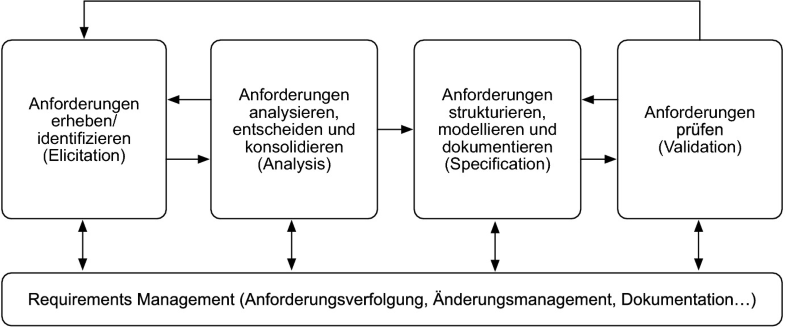
\includegraphics[scale=0.4]{Anforderungsanalyse}}
    \caption{Prozess der Anforderungsanalyse.}
    \label{fig:anforderungsanalyse}
\end{figure}

Wie aus Abbildung \ref{fig:anforderungsanalyse} hervorgeht, ist der Arbeitsprozess der Anforderungsanalyse iterativ und inkrementell. Dies kann in dieser Arbeit nur teilweise umgesetzt werden. Insbesondere die sich wiederholenden Vorgänge dienen dazu, Anforderungen regelmäßig zu überprüfen und letztlich damit einen Entwurf in ein finales Softwareprodukt zu überführen. Diese Aufgabe erfordert ein begleitendes Management (Requirements-Management), da es hier von der konzeptuellen Arbeitsphase in die Organisations- sowie Realisierungsphase geht. Die Konzeption eines offenen Forschungsdatenmanagements bildet hier nur die erste konzeptuelle Phase im Entwicklungsprozess ab. Für die nächsten Schritte der Implementierung wären über die Arbeit hinaus Ressourcen notwendig.  

Mit Open Science und Forschungsdatenmanagement als Rahmenbedingungen von offenem Forschungsdatenmanagement werden im ersten Kapitel die Grundlagen herausgearbeitet und der Forschungsstand überblickt, der den gegenwärtigen Ist-Stand von Umsetzungsmöglichkeiten vor allem auf der technischen Ebene aufzeigt. Im zweiten Kapitel wird zuerst die inhaltliche Einordnung der Forschungsdaten zu Jüdischen Gewerbebetrieben in das Forschungsfeld zur Vernichtung der wirtschaftlichen Existenz der Juden im Nationalsozialismus vorgenommen. Daran anknüpfend werden inhaltliche Kriterien entwickelt, die das \textit{offene} Forschungsdatenmanagement im Kontext des Forschungsfelds klar definieren und dessen Leistungsumfang grundlegend abstecken. Anschließend wird sich mit weiteren Voraussetzungen, die das offene Forschungsdatenmanagement parametrisieren, auseinandergesetzt. Dazu gehören die Interessengruppen (Stakeholder), die grundsätzliche Bereitschaft zu Open Science sowie die rechtlichen und ethischen Rahmenbedingungen. Zur Identifizierung der Interessengruppen (Stakeholder) sowie zur Erhebung der forschungsfeldspezifischen Anforderungen wurden vier Experteninterviews durchgeführt und mit basalen qualitativen inhaltsanalytischen Techniken in einem Mix-Method-Verfahren ausgewertet. Hierbei erfolgte anhand eines Fragenkatalogs eine deduktive Hauptkategorienbildung, welche durch induktiv gebildete Subcodes ergänzt wurde.\footnote{Das Codesystem und die Transkripte sind im Anhang D.4 beigefügt.} Abschließend wird eine prototypische Lösung des offenen Forschungsdatenemanagements am Beispiel der Forschungsdaten zu Jüdischen Gewerbebetrieben entwickelt. Hierbei wird der gewählte Lösungsansatz diskutiert bevor im nächsten Schritt das offene Forschungsdatenmanagement an einem idealtypischen Forschungsprozess entlang strukturiert, modelliert und dokumentiert wird.\\ \\
Im Sinne ihres Themas wurde die Arbeit offen erarbeitet und ist auf der \textit{Open Science Framework}-Plattform vollumfänglich zugänglich.\footnote{Weitere Ausführungen dazu im Anhang D.1.}



\singlespacing 
\chapter{Grundlagen}
\onehalfspacing
Open Science gewinnt auf wissenschaftlicher sowie auf wissenschafts- und gesellschaftspolitischer Ebene an Bedeutung.
Open Science zwar ein positiv besetzter und vielfach benutzter Begriff ist, aber bei genauerem Hinsehen pauschal kein Selbstläufer ist
Forschungsstand zu Open Science und Forschungsdatenmanagement
Open Science in Zusammenhang mit Forschungsdaten und Forschungsdatenmanagement praktiziert werden kann. Nach einem allgemeinen Überblick über Ursachen, Ziele und Konzepte von Open Science, wird anschließend auf Open Data fokussiert und 
Hier wird im Weiteren untersucht in welchem Verhältnis Open Data zum noch relativ jungen Forschungsfeld des Forschungsdatenmanagements (FDM) steht, das bezüglich digitaler Forschungsdaten in den letzten Jahren an Bedeutung in der Wissenschaft gewonnen hat. Dazu wird das Forschungsfeld selbst kurz überblickt. Zum Schluss bleibt das dritte Foschungsfeld der Vernichtung der wirtschaftlichen Existenz der Juden im Nationalsozialismus, an dem exemplarisch anhand von Foschungsdaten zur Vernichtung der jüdischen Gewerbetätigkeit der Bedarf sowie Anforderungen an offenes Forschungsdatenmanagement, welches Open Science-Ansätze integriert, analysiert werden.


Auch wenn von der Replikationskrise nicht direkt betroffen, so stellt sich die Frage nach Qualitätssicherung von wissenschaftlicher Forschung und Arbeit ebenso für die Geschichtswissenschaften - gerade in der digitalen Transformationphase, die tiefgreifende Veränderungen in der Forschungspraxis mit sich bringt. Die selbstkritische Haltung der Open Science-Bewegung gegenüber der eigenen Disziplin wird in dieser Arbeit aufgegriffen und deren abgeleitete Lösungsstrategien aufgenommen.



über den historiographischen Kontext Klarheit verschafft zur Einordnung der hier betrachteten historischen Forschungsdaten

Hinsichtlich der Verfahren und Strategien nicht alle der gesamten Open Science Taxonomie erläutern, sondern in Bezug auf Thema der Arbeit auf Forschungsdaten beschränken. Open Data und FAIR-Data, wo letztere seinen Ursprung aus dem Feld des FDM kommt  

Um ein solches offenes FDM in dieser Arbeit im Sinne der Praktikabilität und Überschaubarkeit im Griff zu behalten, muss es allerdings auch klar abgegrenzt sein. Hier bietet sich die Fokussierung auf einen handhabbaren thematischen Rahmen an, dessen Grenzen also zwischen wissenschaftlicher Schlüssigkeit/ Nachvollziehbarkeit und pragmatischer Machbarkeit ausloten. In einem ersten Schritt wird daher zur thematischen Einordnung der größere  historiographische Kontext dargestellt, in dem sich das offene FDM bewegt. Darauf folgt die thematische Eingrenzung auf Forschungsfeld zur Vernichtung der jüdischen Gewerbetätigkeit im Nationalsozialismus. Dieses bildet den Kontextrahmen, in dem das offene FDM zukünftig arbeiten wird und dessen Merkmale in einem Überblick vorgestellt werden.

FDM weist große Schnittmengen zu Open Science auf, daher es schlussfolgernd nur konequent ist, die beiden Gebiete zusammen zu denken. FDM greift Open Science-Ansätze auf

FDM
- Infrastrukturen im Aufbau
- Orientierung am datenlebenszyklus
- Umsetzung der FAIR Data Prinzipien, Abgrenzung zu Open Data, und nach Möglichkeit Open Research Data

\section{Open Science}

Was das Schlüsselwort ,,Open'' im Kontext von Wissenschaft aussagt, erschließt sich nicht sofort. Um zu verstehen, was Open Science ist und warum diese als notwendig für die traditionelle Wissenschaft gewertet wird, wird die gleichnamige Bewegung in den Blick genommen und deren Ursprünge überblickt.\footnote{Genau genommen ist das Konzept von Open Science, also im Kern eigene Forschungsmethoden,  -praktiken und -ergebnisse transparent für andere zu machen, schon älter und findet Anwendung bereits in der Renaissance. Für das Thema dieser Arbeit ist eine longue durée letztlich wissenschaftlicher Praxis jedoch nicht relevant. Daher wird sich auf die aktuelle Bewegung und deren direkte Ursprünge begrenzt. Siehe auch Paul A. David: Common Agency Contracting and the Emergence of ,,Open Science'' Institutions, in: The American Economic Review (Hrsg.), 2. Ausgabe, 1998, S. 15–21, URL (stable): \url{http://www.jstor.org/stable/116885.}.} Zudem wird der Versuch unternommen, den Begriff Open Science für eine Anwendung in dieser Arbeit zu definieren. Anhand von existierenden Konzepten und Infrastruktuen wird abschließend herausgearbeitet, wo Open Science gegenwärtig steht, woraus sich wiederum Konsequenzen für die Implementierung eines offenen Forschungsdatenmanagements ergeben. 

\subsection{Ursprünge der Open Science-Bewegung}

Hinsichtlich der Entstehung der Open Science-Bewegung können zwei Entwicklungsstränge verfolgt werden. Zum einen lässt sie sich auf ein konkretes Ereignis innerhalb der Wissenschaft zurückverfolgen, nämlich auf die sogenannte Replikationskrise. Hier bezieht sich Open Science explizit auf die Transformation wissenschaftlicher Forschungsmethoden und -praktiken, um Forschung noch robuster zu machen. Zum anderen ist Open Science Teil der breiteren sozialen Open-Bewegung, welche von der Do-it-yourself-Bewegung, der Hacker-Bewegung der 1960/ 70er sowie der Freie-Software-Bewegung der 1980er Jahre
(Vorgänger der Open Source-Bewegung) stark beeinflusst ist.\footnote{Vgl. ayway media (Hrsg.): Das digitale Handbuch,
Kapitel C.15 Die ,,Open-Bewegung'', Vettelschloss 2016, S. 252}

\paragraph{Replikationskrise} Ab Mitte der 2010er Jahre erhielten in der Wissenschaft, vordergründig in der Psychologie sowie in den Lebens- und Naturwissenschaften, zunehmend Replikationsstudien Aufmerksamkeit. Diese konnten in sogenannten Replikationsversuchen eine statistisch signifikante Anzahl publizierter empirischer Forschungsergebnisse entweder falsifizieren oder nicht replizieren, weil die Daten nicht zur Verfügung standen.\footnote{Als erste Replikationsstudie dieser Art wird jene des Medizinwissenschaftlers und Statistiskers John Ioannidis aus dem Jahr 2005 gezählt, mit der er erstmals systematisch versuchte, veröffentlichte Untersuchungsergebnisse nachträglich zu replizieren/ reproduzieren. Siehe John P.A. Ioannidis: Why Most Published Research Findings Are False, PLoS Med 2(8): e124, 2005, doi:10.1371/journal.pmed.0020124. Es folgten eine Reihe weiterer Replikationsstudien auch in anderen Fächern wie den Sozialwissenschaften. Siehe zum Beispiel Marjan Bakker, Annette van Dijk, Jelte M. Wicherts: The Rules of the Game Called Psychological Science, in: Perspectives on Psychological Science, 7(6), 2012, S. 543-554, doi:10.1177/1745691612459060; Thomas Herndon, Michael Ash, Robert Pollin: Does high public debt consistently stifle economic growth? A critique of Reinhart and Rogoff, in: Cambridge Political Economy Society (Hrsg.), Cambridge Journal of Economics, Band 38, 2. Ausgabe, Oxford 2014, S. 257-279, URL (stable): \url{https://www.jstor.org/stable/24694929}; Jeremy Freese, David Peterson: Replication in Social Science, in: Annual Reviews (Hrsg), Annual Review of Sociology, Band 43, San Mateo 2017, S. 147-165, doi:10.1146/annurev-soc-060116-053450} Das löste die vielfach diskutierte ,,Replikationskrise'' in den betroffenen Fächern aus. Zum einen ging es, hinsichtlich der Falsifizierungen, nachträglich um Ursachenforschung, die sich auf Defizite insbesondere bei den Forschungsmethoden und in der Publikationspraxis wissenschaftlicher Journals fokussierte.\footnote{Diskutiert wurden insbesondere, wie das Institut für Psychologie an der Humboldt-Universität zu Berlin konzis berichtete, "p-hacking, selektives Berichten von (abhängigen) Variablen, Hypothesizing After the Results are Known (HARKING), nur signifikante Ergebnisse berichten, mehr Daten sammeln nachdem die bestehenden Daten keine positiven Ergebnisse hervorgebracht haben, Publikations Bias". Methodengruppe Berlin (Autorengruppe): Die Replikationskrise und Open Science, Blog Post, Humboldt-Universität zu Berlin, Lebenswissenschaftliche Fakultät Institut für Psychologie, Lehrstuhl für Psychologische Methodenlehre (Hrsg), URL: \url{http://methods-berlin.com/de/replikationskrise_open_science/} (letzter Zugriff am 21.04.2022). Siehe auch Klaus Fiedler, Norbert Schwarz: Questionable Research Practices Revisited, in: SAGE Publishing (Hrsg.), Social Psychological and Personality Science, Band 7, 1. Ausgabe, 2016, S. 45-52, doi:10.1177/1948550615612150; Annie Franco, Neil Malhotra, Gabor Simonovits: Publication bias in the social sciences. Unlocking the file drawer, in: American Association for the Advancement of Science (Hrsg.), Science, Band 345, Ausgabe 6203, Washington 2014, S. 1502-1505, doi:10.1126/science.1255484.} Aber auch die Replikationsstudien selbst wurden kritisch betrachtet.\footnote{Vgl. Deutsche Forschungsgemeinschaft (Hrsg.): Replizierbarkeit von Forschungsergebnissen. Eine Stellungnahme der Deutschen Forschungsgemeinschaft, Stand: April 2017, URL: \url{https://www.dfg.de/download/pdf/dfg_im_profil/geschaeftsstelle/publikationen/stellungnahmen_papiere/2017/170425_stellungnahme_replizierbarkeit_forschungsergebnisse_de.pdf} (letzter Zugriff am 21.04.2022).} Zum anderen war, hinsichtlich der Nichverfügbarkeit von Daten, eine wesentliche Eigenschaft von robuster evidenzbasierter Forschung, nämlich die Nachvollziehbarkeit ihrer Ergebnisse durch Replikation (als Bestandteil von Qualitätssicherung), nicht mehr gegeben und damit in der Konsequenz auch ein gesellschaftlicher Bedeutungsverlust von Wissenschaft bei der Wissensproduktion zu befürchten. 

Kurzum ging es um die existenzielle Frage, wie Wissenschaft praktiziert werden muss, damit wissenschaftliche Forschung, insbesondere die statistisch empirische, reliabel ist. Als Antwort auf diese Krise hat sich in den vergangenen Jahren die internationale Open Science-Bewegung formiert\footnote{Entsprechend der Internationalität der Open Science-Bewegung, existieren weltweit Open Science Initiativen, von denen allein in Deutschland hier nur eine Auswahl wiedergegeben werden kann: Berlin School of Public Engagement and Open Science als Kollaborationsprojekts des Museums für Naturkunde Berlin, der Humboldt-Universität zu Berlin und der Robert-Bosch-Stiftung, URL: \url{https://www.museumfuernaturkunde.berlin/de/future/wissenschaftscampus/berlin-school-public-engagement-and-open-science}; Open Science Working Group an der FU Berlin, URL: \url{https://www.fu-berlin.de/sites/open-science}; Open Science Center an der LMU München;  Initiative für Offene Wissenschaft und Innovation des Stifterverbands, URL: \url{https://www.stifterverband.org/open-science-innovation-netzwerke}.}, die in den Anfangsjahren stark auf die Frage nach Replizierbarkeit von Forschungsstudien fokussiert war. 

In Deutschland hat sich zuletzt das \textit{German Reproducibility Network} (GRN) gegründet, das fachübergreifend gezielt Replikationsstudien und Open Science Praktiken unterstützen möchte.\footnote{Zu dessen Hauptakteuren gehören u.a. Berlin University Alliance, das Helmholtz Center (Open Science), das LMU Open Science Center (OSC), das Netzwerk der Open Science Initiativen (NOSI), die Deutsche Gesellschaft für Psychologie (DGPs), u.a. Siehe Ankündigung der Berlin University Alliance: German Reproducibility Network gestartet, News vom 01.02.2021, URL: \url{https://www.berlin-university-alliance.de/news/items/2021/210201-grn.html}. Homepage des GRN unter URL: \url{https://reproducibilitynetwork.de/} (alle letzter Zugriff am 27.04.2022).} Auf internationaler Ebene ist vor allem das interdisziplinäre \textit{Center for Open Science} (COS) zu nennen, welches in direkter Reaktion auf die Replikationskrise 2013 in den USA gegründet wurde\footnote{URL: \url{https://www.cos.io/?hsLang=en} (letzter Zugriff am 21.04.2022).}. Eine der ersten Aktivitäten des COS war das mit der University of Viginia gemeinsam großangelegte \textit{Reproducibility Project}, in dem sich eine Autorengruppe, welche sich ,,Open Science Collaboration'' nannte, systematisch mit der Reproduzierbarkeit von 100 Forschungsstudien in der Psychologie auseinandersetzte.\footnote{Brian A. Nosek, Johanna Cohoon, Mallory C. Kidwell, Jeffrey R. Spies: Estimating the reproducibility of psychological science, in: American Association for the Advancement of Science (Hrsg.), Science, Band 349, Ausgabe 6251, Washington 2015, doi:10.1126/science.aac4716.}. Nach der Bestandsaufnahme, bei der die Rate nichtreplizierbarer Forschungsstudien wie bei vorausgegangenen Replikationsstudien signifikant hoch war, widmete sich das COS verstärkt den Strategien zur Überwindung der Replikationskrise, die im Kern ebenfalls als eine methodische Krise identifiziert wurde sowie zweifelhafte Forschungspraktiken aufdeckte.

\paragraph{Open-Bewegung} Die Open Science-Bewegung ist Teil der breiten sozialen Open-Bewegung, welche unter den Begriffen ,,Open'', ,,Openness'' beziehungsweise ,,Free'' subsumiert, ,,Daten, Entwürfe, Fotos, Musikstücke oder sonstige Inhalte und Wissen'' \footnote{Wikimedia Deutschland e. V., Open Knowledge Foundation Deutschland e. V. (Hrsg.): ABC der Offenheit, Berlin 2019, S. 4f., URL: \url{https://commons.wikimedia.org/wiki/File:ABC_der_Offenheit_-_Broschüre_(2019).pdf} (letzter Zugriff am 26.04.2022).} aus allen gesellschaftlichen Bereichen zur Weiterverbreitung sowie Wiederverwendbarkeit schrankenlos zur Verfügung stellen und dadurch Teilhabe als demokratisches Prinzip in einer freiheitlichen Gesellschaft stärken will. Außerdem sieht sie in dieser Kultur der Offenheit Potenzial für neue Innovationen\footnote{Ebd. sowie siehe auch Open Knowledge Foundation (Hrsg.): Why open data? URl: \url{https://okfn.org/opendata/why-open-data/} (letzter Zugriff am 26.04.2022).} Diese Forderungen sind zwar nicht grundsätzlich neu, bekamen aber mit der Verbreitung des World Wide Web (WWW) ab Mitte der 1990er Jahre\footnote{Veröffentlichung des ersten Webbrowsers Netscape in offener Lizenz, die Personen auf der ganzen Welt mit PC und Internetverbindung ermöglichte, frei im Web ,,zu surfen''} einen neuen Schub. Dies ist in der Natur des WWW selbst begründet. Denn dessen Schlüsseleigenschaft ist es - seit seiner Entstehung 1989 - Informationen system- und plattformunabhängig in einer gemeinsamen Netzwerkinfrastruktur zu übertragen und auszutauschen.\footnote{Erfunden wurde das WWW vom Physiker und Informatiker Tim Berners-Lee, der 1989 am CERN in Genf arbeitete und technischen Lösungen suchte, wie unter Forschern schnell und einfach kommuniziert werden kann. Die grundlegenden Technologien des WWW waren und sind es bis heute: HTML zur Darstellung und Verlinkung von Informationen (Hyper Text Markup Language), URI/ URL (Unified Ressource Identifier bzw. Locator) zur Lokalisierung einer Ressource z.B. eines HTML-Dokuments im Rechnernetz, HTTP (Hyper Text Transfer Protocol) zur Übertragung dieser Ressource im Rechnernetz. Zur detaillierten Historie, Funktionsweise und weiteren Entwicklung des WWW siehe zum Beispiel Tim Berners-Lee, Mark Fischetti: Weaving the web. The original design and ultimative destiny of the World Wide Web by its inventor, New York 2011. Niels Brügger: Web history, New York, Bern 2010. James Gilles, Robert Cailliau: How the Web was born. The story of the World Wide Web, Oxford University Press, 2000.} Damit eignete es sich auch, die Forderungen der Open-Bewegung technisch zu implementieren. Folglich werden überwiegend webbasierte Technologien in der Open-Bewegung eingesetzt, insbesondere die des Web 2.0, welche die Interaktionsmöglichkeiten im digitalen Raum erheblich erweiterten.\footnote{Vgl. Benedikt Fecher, Sönke Friesike: Open Science. One Term, Five Schools of Thought, Springer, 2014, S.11, doi:10.1007/978-3-319-00026-8\_2.} Eine wichtige Voraussetzung für viele heutige Open (Science) Projekte war zudem, dass die Technologien hinter dem WWW selbst von Anfang an offen waren, diese also (kosten)frei für jeden zur Verfügung standen und von jedem genutzt werden konnten.\footnote{Der Begründer Tim Berners-Lee hat sich von Anfang dafür eingesetzt das WWW offen zu halten. Er gründete 2012 in London das gemeinnützige Open Data Institute (ODI) mit, wodurch er selbst ein (einflussreicher) Vertreter der Open-Bewegung ist. URL: \url{https://theodi.org/} (letzter Zugriff am 27.04.2022).} 

Die Open Science-Bewegung kann in diesem Kontext als Weiterentwicklung der vor 20 Jahren gegründeten Open Access-Bewegung gesehen werden, in der sich Wissenschaftler*innen 2002/2003 zusammengeschlossen haben, um offenen Zugang zu wissenschaftlichen Forschungsergebnissen zu fördern.\footnote{Siehe Erklärung der ,,Budapest Open Access Initiative'' vom 14.02.2002, URL: \url{https://www.budapestopenaccessinitiative.org/read/} sowie ,,Berliner Erklärung über den offenen Zugang zu wissenschaftlichem Wissen'' vom 22. Oktober 2003, abgerufen auf der Website der Max Planck Gesellschaft, URL: \url{https://openaccess.mpg.de/Berliner-Erklaerung} (alle letzter Zugriff am 02.05.2022)} Daneben umfasst die Open-Bewegung unter anderem Open Knowledge, Open GLAM, Open Government, Open Design, Open Innovation, wobei es eine trennscharfe Abgrenzung nicht gibt. So lässt sich Open Data auch als Querschnittsbereich auffassen, der in andere Bereiche wie Open Science hineinreicht.\footnote{Vgl. Birgit Schmidt, Astrid Orth, Gwen Franck, Iryna Kuchma, Petr Knoth, José Carvalho: Stepping up Open Science Training for European Research, in: Publications (Hrsg), 2 Ausgabe, 2016, S. 3, doi:10.3390/publications4020016. Eine konzise Übersicht aller Bereiche siehe auch WMK, OKF (2019), ABC der Offenheit, S. 14-54}. Eine Vertreterin der ersten Stunde der Open-Bewegung und die wohl populärste ist die gemeinnützige Wikimedia Foundation, Inc. (WMF)\footnote{URL: \url{https://wikimediafoundation.org/de/} (letzter Zugriff am 22.04.2022)} mit Sitz in den USA.\footnote{Vgl. den Wikipedia-Eintrag zur Wikimedia Foundation, Seite ,,Wikimedia Foundation''. In: Wikipedia – Die freie Enzyklopädie. Bearbeitungsstand: 31. März 2022, 20:07 UTC. URL: \url{https://de.wikipedia.org/w/index.php?title=Wikimedia_Foundation\&oldid=221669459.} (letzter Zugriff am 22.04.2022) In Deutschland vertreten durch den Verein Wikimedia Deutschland e. V., vgl. ebd.} Bereits seit 2001 stellt sie digitale Dienste kostenfrei zur Verfügung, mit denen Wissen offen ausgetauscht und geteilt werden kann. Ihr bekanntestes und ältestes Projekt ist die freie Enzyklopädie \textit{Wikipedia}\footnote{URL: \url{https://de.wikipedia.org/wiki/Wikipedia:Hauptseite} (letzter Zugriff am 22.04.2022)}. Die WMF engagiert sich aber nicht ausschließlich mit der Wikipedia in der Open-Bewegung, sondern hat inzwischen eine Vielzahl an digitalen ,,Schwesternprojekten''\footnote{Zum Beispiel das Wörterbuch Wictionary (2002), URL: \url{https://de.wiktionary.org/}; die Text- und Quellensammlung Wikisource (2003), URL: \url{https://de.wikisource.org/wiki/Hauptseite}; die Mediensammlung Wikimedia Commons (2004), URL: \url{https://commons.wikimedia.org/wiki/Hauptseite}; die Wissensdatenbank Wikidata (2012), URL: \url{https://www.wikidata.org/wiki/Wikidata:Main_Page} (alle letzter Zugriff am 22.04.2022). Eine Auflistung aller Wikimedia-Projekte ist auf der Homepage zu finden unter \url{https://www.wikimedia.de/projekte/} (letzter Zugriff am 22.04.2022)} Daneben stellt sie eine Reihe ihrer MediaWiki Software-Komponenten in Open Source zur Verfügung.\footnote{Eine Übersicht ist auf der Website zu finden unter URL: \url{https://doc.wikimedia.org/} (letzter Zugriff am 22.04.2022)} Eine weitere und mit der WMF koopierende Organisation in der Open-Bewegung ist die Open Knowledge Foundation (OKF), die 2005 in London gegründete wurde\footnote{URL: \url{https://okfn.org/} (letzter Zugriff am 22.04.2022).} und von der es seit 2011 auch einen deutschen Ableger in Berlin gibt.\footnote{URL: \url{https://okfn.de/} (letzter Zugriff am 22.04.2022).}. Anders als die WMF hat die OKF kein zentrales Projekt mit einer homogenen Softwarelandschaft, sondern wirkt unterstütztend und begleitetend an kleineren Projekten.\footnote{Siehe Open Knowledge Foundation (Hrsg.): What we do? URL: \url{https://okfn.org/what-we-do/} (letzter Zugriff am 26.04.2022).}

Beide hier vorgestellten Initiativen engagieren sich ebenfalls in der Open Science. An der deutschsprachige OKF hat sich die Arbeitsgruppe Open Science gegründet, die wiederum von der Wikimedia Deutschland unterstützt wird.\footnote{Siehe Website der AG Open Science, URL: \url{https://ag-openscience.de/netzwerk/} (letzter Zugriff am 03.05.2022).} In der offenen AG kommen unterschiedliche Akteure aus der Wissenschaft zusammen, die gemeinsam Open Science-Ziele für die Wissenschaft formulieren.\footnote{Vgl. Open Science AG (Hrsg.): Mission Statement. Science - Open by default, Verison 1.0, Oktober 2014, URL: \url{https://ag-openscience.de/mission-statement/} (letzter Zugriff am 03.05.2022).} Die Wikimedia Deutschland gibt die Blogreihe „Freies Wissen und Wissenschaft“ heraus, in der bisher Stärken und Vorteile von Open Science für die traditionelle Wissenschaft herausgearbeitet wurden.\footnote{Wikimedia Deutschland (Hrsg.): Freies Wissen und Wissenschaft, Blogreihe, Teil 01-07, URL: \url{https://blog.wikimedia.de/2015/04/20/freies-wissen-und-wissenschaft-teil-01-science-2-0-die-digitalisierung-des-forschungsalltags/} (letzter Zugriff am 03.05.2022).} Außerdem hat sie zwischen 2016 und 2021 das interdisziplinäre Fellow-Programm \textit{Freies Wissen} durchgeführt, mit dem Nachwuchswissenschaftler*innen bei der Integration von Open Science in das eigene Forschungsprojekt gefördert wurden.\footnote{Sarah Behrens, Christopher Schwarzkopf, Anna-Katharina Gödeke, Dr. Dominik Scholl, Nico Schneider (2022): Fellow-Programm Freies Wissen 2016 - 2021, Zenodo, doi:10.5281/zenodo.5788379. Siehe auch Informations- und Kommunikationskanäle des Fellow Programms auf de.wikimedia.org, URL's: \url{https://www.wikimedia.de/projects/fellow-programm-freies-wissen/}, \url{https://de.wikiversity.org/wiki/Wikiversity:Fellow-Programm_Freies_Wissen}, \url{https://blog.wikimedia.de/c/fellow-programm-freies-wissen-de/} (alle letzter Zugriff am 03.05.2022)} Mit diesem Zugriff auf die Wissenschaft war der Effekt des Programms auch, dass Open Science-Multiplikatoren ausgebildet wurden, die die Idee und Praxis von Open Science in wissenschaftlichen Einrichtungen und Communities verbreiten und festigen.\footnote{Vgl. Moritz Schubotz, Isabella Peters, Benedikt Fecher, Dominik Scholl (2020): Lessons Learned aus dem Fellow-Programm Freies Wissen. Open-Access-Tage 2020 (OAT2020), Bielefeld, Germany, Zenodo, doi:10.5281/zenodo.4009144}

\subsection{Definition} 

Eine allgemeingültige Definition von Open Science, die hier eins zu eins übernommen werden kann, existiert nicht.\footnote{Bestätigt wird diese Aussage von dem öffentlichen Wiki ,,forschungsdaten.org'' der Universität Koblenz, welches seit 2019 von der Universität betrieben wird (vorher vom Helmholtz-Zentrum Potsdam und Deutschem GeoForschungsZentrum GFZ), in dem allein 11 Definitionen vorgstellt werden, vgl. URL: \url{https://www.forschungsdaten.org/index.php/Open_Science} (letzter Zugriff am 30.04.2022).} Erschwerend kommt hinzu, dass ebenfalls die Open Research oder Open Scholarship oft, aber nicht immer synonym verwendet werden.\footnote{Siehe zum Beispiel Freie Universität Berlin (Hrsg.): FDM Glossar. Open Science\/ Open Research\/ Open Scholarship, URL: \url{https://www.fu-berlin.de/sites/forschungsdatenmanagement/glossar/open-science-open-research-open-scholarship.html}, Ben Kaden: Drei Gründe für Forschungsdatenpublikationen, Blogartikel auf eDissPlus, DFG-Projekt: Elektronische Dissertationen Plus, 29.09.2016, URL: \url{https://www2.hu-berlin.de/edissplus/2016/09/29/gruende-fuer-forschungsdatenpublikationen/} (alle letzter Zugriff am 30.04.2022).} Hieraus ergibt sich ein Definitionsproblem für diese Arbeit, das sich aus dem IST-Stand von Open Science ergibt. Denn entsprechende Verfahren und Strukturen sowohl auf der technischen als auch auf der organisatorischen Ebene haben sich schlichtweg noch nicht etabliert. Zwar gibt es - wie der vorherige Abschnitt gezeigt hat - ein großes Bekenntnis zu Open Science, doch die feste Verankerung in das bestehende Wissenschaftssystem ist noch nicht erfolgt. Erst aber in diesem Prozess wird sich Open Science abschließend konsolidieren. 

Es können aber die sogenannten Open Science-Grundsätze als ,,weiche'' Definition und als Handlungsrahmen für diese Arbeit herangezogen werden. Sie werden von allen recherchierten Initiativen vorgetragen und können wie folgt zusammengefasst werden: Während von wissenschaftlicher Seite insbesondere Transparenz, offene Kommunikation, Kollaboration, Reproduzierbarkeit und Wiederverwendbarkeit in der Forschung betont wird, ist es von der Open-Bewegung her vor allem öffentliche Partizipation, die zentral ist. Open Science wird als moderne Wissenschaftspraxis gesehen, die traditionelle Wissenschaft dort transformiert, wo es - wie die Replikationskrise gezeigt hat - notwendig ist. Das primäre Ziel ist es, durch Open Science Integrität von Wissenschaft zu stärken, Qualität von Forschung im digitalen Zeitalter zu steigern und Wissenschaft selbst zu demokratisieren.\footnote{Vgl. Ina Friebe: Forschungsqualität durch Open Science verbessern, veröffentlicht auf der Website der Berlin University Alliance (Hrsg.) am 12.05.2021, URL: \url{https://www.berlin-university-alliance.de/impressions/210512-lecture-series-o3/index.html} (letzer Zugriff am 27.04.2022).} Eine wichtige Eigenschaft dieser Grundsätze ist zudem, dass sie generisch, das heißt über alle wissenschaftlichen Domänen hinweg gültig sind.\footnote{Vgl. CODATA Coordinated Expert Group, Paul Arthur Berkman, Jan Brase, Richard Hartshorn, Simon Hodson, Wim Hugo, Sabina Leonelli, Barend Mons, Hana Pergl, Hans Pfeiffenberger: Open Science for a Global Transformation: CODATA coordinated submission to the UNESCO Open Science Consultation. Zenodo 2020, Version 1, S. 13 doi:10.5281/zenodo.3935461.} Von daher spricht Open Science nicht allein die lebens- und naturwissenschaftlichen Bereiche, sondern gleichermaßen auch die geisteswissenschaftlichen an und deren Grundsätze sind folglich auch auf die Forschungsdaten zur Vernichtung der jüdischen Gewerbetätigkeit im NS anwendbar.

Während diese Open Science-Grundsätze (manchmal auch Open Science-Principles) als gesetzt gelten können, bleibt die Antwort auf die Frage nach dem Open Science-Grad, also wie weit Offene Wissenschaft auf den Forschungsprozess ausgedehnt ist, abschließend uneindeutig. Es lassen sich zum jetztigen Zeitpunkt jedoch zwei Gruppen identifizieren und abstufen:
\begin{enumerate}
\item Grad: Auf der einen Seite können die Akteure zusammengefasst werden, die unter Open Science die Veröffentlichung aller Forschungs\textit{ergebnisse} verstehen.\footnote{Siehe zum Beispiel die Selbstverständnis-Erklärung des Arbeitskreises Open Science der Helmholtz-Gemeinschaft, URL: \url{https://os.helmholtz.de/open-science-in-der-helmholtz-gemeinschaft/stakeholder-und-ihre-rollen/arbeitskreis-open-science/selbstverstaendnis-des-arbeitskreises-open-science-der-helmholtz-gemeinschaft/} (letzter Zugriff am 01.05.2022). Auch das öffentliche Zenodo-Repositorium wird vielfach so verwendet, vgl. Kapitel 2.1.3 Infrastrukuren.} Sie sehen den Fortschritt in Open Science darin, dass nicht mehr textbasierte Publikationen wie wissenschaftliche Artikel, Monografien, Editionen, etc. zugänglich sind, sondern ebenfalls alle digitalen Ressourcen, wie Daten oder Software, die epistemologischen Wert besitzen, also zu den gewonnen Erkenntnissen beigetragen haben. Diese digitalen Ressourcen werden als Teil der Forschungsergebnisse interpretiert und diese müssen in der Konsequenz veröffentlicht werden. Der traditionelle Forschungsprozess an sich bleibt größtenteils unberührt. Lediglich dessen abschließende Phase, wenn es darum geht Ergebnisse zu kommunizieren, soll erweitert werden und hier Zugänglichkeit und Wiederverwendbarkeit von Forschungsergebnissen gefördert werden.
\item Grad: Auf der anderen Seite stehen die Akteure, vor allem aus dem Dunstkreis der Replikationskrise, die hier noch sehr viel weiter als oben genannte Akteure gehen. Denn sie wollen die Open Science-Grundsätze auf alle Phase des Forschungszyklus angewandt sehen und damit den gesamten Forschungsprozess transparent machen. Aus der Erfahrung der Replikationskrise heraus ist ihr Hauptargument, dass es, um Reliabilität von Wissenschaft zu gewährleisten, nicht ausreicht, nur publizierte Forschungsergebnisse zur Verfügung zu haben.\footnote{Vgl. Benedikt Fecher, Mathis Fräßdorf, Marcel Hebing, Gert G. Wagner: Replikationen, Reputation und gute wissenschaftliche Praxis, in: Information - Wissenschaft \& Praxis (Hrsg.), Bd. 68, Ausgabe 2-3, 2017, S. 154-158, doi:10.1515\/iwp-2017-0025.} Dabei stimmt sie den Forderungen der ersten Gruppen grundsätzlich zu, erweitert diese aber, indem sie die Praxis des Veröffentlichens ausschließlich \textit{publizierbarer} Forschungsergebnisse aufbrechen will. Genau hierin liegt der entscheidende Unterschied zu den Akteuren der ersten Gruppe. Denn bei dieser konsequenten Umsetzung der Open Science-Grundsätze, würden auch alle Rohdaten und Working Papers - also die Zwischenergebnisse -, vor ihrer Bereinigung bzw. vor dem Peer-Review, sowie dokumentierte Workflows der Forschungsarbeit mit Methodenentwicklung und Forschungsdesign zugänglich sein. Erst auf diese Weise - so die Argumentation - lasse sich der gesamte Erhebungs-, Verarbeitungs- sowie Analysesprozess von Forschungsdaten und damit der Erkenntnisprozess selbst in größtmöglicher Transparenz nachvollziehen und befähigt im Sinne einer Datenkritik, sowohl die Daten als auch die Ergebnisse nachträglich zu beurteilen und abschließend zu bewerten, was insbesondere für deren Nachnutzung von epistemologischer Bedeutung ist.\footnote{Und auch von lebensrettender Bedeutung, wie im Zusammenhang mit der COVID-19-Pandemie seit 2020 vielfach diskutiert wird. Den Open Science-Kerneigenschaften wie der globale ungehinderte Austausch von Daten, Papers und Zwischenergebnissen werden eine entscheidende Rolle bei der raschen Impfstoffentwicklung zugewiesen. Siehe Lonni Besançon, Nathan Peiffer-Smadja, Corentin Segalas, Haiting Jiang, Paola Masuzzo, Cooper Smout, Eric Billy, Maxime Deforet, Clémence Leyrat: Open science saves lives: lessons from the COVID-19 pandemic, in: BMC Medical Research Methodology, Band 21, Artikelnr. 117, 2021, doi:10.1186/s12874-021-01304-y und CODATA Coordinated Expert Group (2020): Open Science for a Global Transformation. CODATA coordinated submission to the UNESCO Open Science Consultation, Zenodo, doi:10.5281/zenodo.3935461.} 
\end{enumerate}  

Die vorgestellten Diffenzierungen von Open Science machen deutlich, dass es \textit{die} Open Science nicht gibt und bis zu welchem Grad sich Open Science am Ende durchsetzen wird, muss in dieser Arbeit offen bleiben. Letztendlich hängt diese Entwicklung stark vom Selbstverständnis der jeweiligen Initiatve, Einrichtung oder des jeweiligen Wissenschaftsbereichs sowie von anderen Variablen wie rechtliche oder forschungsethische Rahmenbedingungen ab. Es ist daher wahrscheinlich, dass sich Open Science unter der gemeinsamen Klammer der Open Science-Grundsätze zukünftig weiter ausdifferenzieren wird und unterschiedliche Grade nebeneinander existieren werden.

\subsection{Konzepte und Infrastrukturen} 

\paragraph{Konzepte}

In Bezug auf Konzepte wird häufig der \textit{Umbrella Term} herangezogen, um die verschiedenenen Open Science-Handlungsfelder in der Wissenschaft zu veranschaulichen and damit die Dimensionen von Open Science zu verdeutlichen (Abb. 2.1.). 

\begin{figure}[h]
    \centering
    \frame{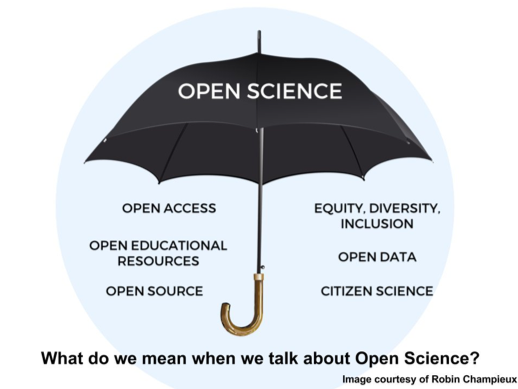
\includegraphics[scale=0.7]{open_science_eosc-hub}}
    \caption{Definition der Open Science-Handlungsfelder nach der Europäischen Kommission.\protect\footnotemark}
    \label{fig:x cubed graph}
\end{figure} \footnotetext{URL: \url{https://www.eosc-hub.eu/open-science-info} (letzter Zugriff am 03.05.2022).}

Die Europäische Kommission zum Beispiel definiert für das große EU-Infrastrukturprojekt ,,European Open Science Cloud'' (EOSC)\footnote{Siehe Abschnitt ,,Infrastrukturen''.}, welche im Rahmen des Langzeitprogramms \textit{Horizon Europe} aufgebaut wird\footnote{Horizon Europe startete 2020 und läuft noch bis 2027 mit einem Förderungsumfang von insgesamt 95,5 Milliarden Euro (Phase 2021-27), URL: \url{https://ec.europa.eu/info/research-and-innovation/funding/funding-opportunities/funding-programmes-and-open-calls/horizon-europe_en} (letzter Zugriff am 03.05.2022)}, sechs Handlungsfelder - wie aus der Abbildung 2.1. hervorgeht. Dabei kombinieren die Handlungsfelder Praktiken aus der traditionellen Wissenschaft mit den Open Science-Grundsätzen und entwickeln daraus Lösungskonzepte für die wissenschaftliche Forschung nach Schwerpunkten. Open Data-Konzepte unter dem Dach der Open Science zum Beispiel konzentrieren sich auf den wissenschaftlichen Umgang mit den im Forschungsprozess anfallenden digitalen Forschungsdaten, während sich Open Access-Konzepte mit Fragen des freien Zugangs zu diesen und sonstigen wissenschaftlichen Materialen beschäftigen. Citizen Science-Konzepte entwickeln Lösungen, wie unter Beibehaltung wissenschaftlicher Integrität Partizipation an Wissenschaft gestärkt werden kann.\footnote{Siehe zum Beispiel die Citizen Science-Plattform ,,Bürger schaffen Wissen'', URL: \url{https://www.buergerschaffenwissen.de/} (letzter Zugriff am 03.05.2022).}

\begin{figure}[h]
    \centering
    \frame{
\includegraphics[scale=0.2]{open_science_british-psy-soc}}
    \caption{Definition der Open Science-Handlungsfelder (hier Open Scholarship) nach der Britischen Gesellschaft für Psychologie (The British Psychological Society).\protect\footnotemark}
    \label{fig:x cubed graph}
\end{figure} \footnotetext{URL: \url{https://thepsychologist.bps.org.uk/volume-33/november-2020/bropenscience-broken-science} (letzter Zugriff am 03.05.2022). Zu sehen ist hier auch die unterschiedliche Begriffsverwendungen ,,Open Science'' und ,,Open Scholarship''}

Die Handlungsfelder können voneinander abweichen, wie ein Blick auf die Abbildung 2.2 zeigt. Die Abweichungen zwischen beiden Abbildungen lassen den Schluss zu, dass es ganz ähnlich zum Open Science-Grad letztlich vom konkreten (wissenschaftlichen) Kontext abhängt, welche Handlungsfelder unter Open Science definiert werden und es hier folglich eine strenge Vorgabe nicht gibt. Schließlich hängt diese Definition auch davon ab, wo und ob überhaupt Handlungsbedarf für Open Science gesehen wird. Dass die Replikationskrise dringenden Handlungsbedarf vorwiegend in den Lebens- und Naturwissenschaften offenbart hat, heißt nicht, dass dieser gleichermaßen auch in geisteswissenschaftlichen Fächern gesehen wird, wo vorwiegend hermeneutische Forschungsmethoden angewandt werden, die sich fundamental von den statistisch empirschen der Naturwissenschaften unterscheiden. Das bedeutet im Umkehrschluss, dass Handlungsbedarf gegebenfalls erst noch geschaffen werden muss oder aber - und die Frage muss erlaubt sein - überhaupt nicht notwendig ist. 

\paragraph{Infrastrukturen} Anhand der gegenwärtigen Anwendungsmöglichkeiten von Open Science in der eigenen Forschung können grob\footnote{Technische Überschneidungen sind nicht ausgeschlossen. Die Einteilung orientiert sich an mögliche Nutzungsszenarien.} drei Gruppen von Infrastrukuren unterschieden werden: 1. zentrale, 2. dezentrale und 3. nachgenutzte Infrastrukturen:

\begin{enumerate}
\item Begleitend zur Reproduzierbarkeitsstudie des COS wurde das \textit{Open Science Framework} (OSF)\footnote{URL: \url{https://osf.io/} (letzter Zugriff am 28.04.2022).} entwickelt, das im Hintergrund eine zentrale IT- Infrastruktur über eine Plattform bereitstellt, die bekannte Open Science Verfahren wie Präregistrierung, Preprints und Generierung von Permalinks ermöglicht. Zum Funktionsumfang gehören außerdem Projektversionierung sowie ein generisches Repositorium zum Speichern und Aggregieren multipler Inhalte unterschiedlicher Formaten. Im veröffentlichten, diese Arbeit von Beginn an begleitenden, OSF-Projekt ,,Master thesis: Open Science in History?''\footnote{URL: \url{https://osf.io/sc9yf/?view_only=aa5eb53a48ba4eaab512d049712d704a}, hier nur mit lesendem Zugriff auf das Projekt.} wurde zum Beispiel die LaTex-Version der schriftlichen Arbeit, welche mit Git versioniert und auf GitHub zugänglich ist, und die Zotero-Library mit der verwendeten Literatur über die Add-ons-Funktionalität sowie die prototypische Wikidata-Lösung für offenes Forschungsdatenmanagement als Komponente dem Projekt hinzugefügt. Lokal gespeicherte Materialien wie die Interviewtranskripte (.pdf), der Fragebogen (.pdf) und die Literaturauswertung (.csv) wurden manuell hochgeladen. Dafür stehen verschiedenen Server zur Verfügung, darunter auch in Deutschland (Frankfurt am Main). Heterogene Dienste und verteilte Ressourcen können also im OSF zusammengeführt und dort synchron gehalten werden. Damit ist das OSF im Kern ein Projektmanagement-Tool, das durch eine homogen gestaltete kollaborative Arbeitsumgebung Wissenschaftler*innen dabei unterstützt, automatisierte Open Science-Worklows in den Forschungsalltag zu integrieren und dadurch systematisch Open Science über den gesamten Forschungsprozess praktizieren zu können.\footnote{Vertrauensvorschuss erhält das COS vor allem durch eine konsequent transparente Politik wie zum Beispiel der Veröffentlichung aller Finanzberichte, URL: \url{https://www.cos.io/about/finances} (letzter Zugriff am 28.04.2022).} Dass das OSF steigende Anwenderzahlen insbesondere durch akademische Einrichtungen in den USA verzeichent,\footnote{Zum Beispiel Princeton University, New York University, George Washington University, u.a. Siehe \url{https://osf.io/institutions} (letzter Zugriff am 21.04.2022).}, weist darauf hin, dass es das Potential hat, sich zu einem Standard in diesem Bereich zu entwickeln. Eine mögliche negative Nebenfolge dieser Entwicklung ist die Entstehung einer Plattformabhängikeit, die zum Beispiel im Zusammenhang mit den sozialen Medien inzwischen kritisiert wird und gegen die sich Widerstand regt.\footnote{Gemeint sind hier Plattformen wie Facebook, Twitter, Google, Amazon, etc., wo die momentane Plattformökonomie Monopolstellung und Machtzentrierung fördert. Siehe zu dieser Problematik Justus Haucap: Plattformökonomie. Neue Wettbewerbsregeln –
Renaissance der Missbrauchsaufsicht, in: Wirtschaftsdienst 100 (Hrsg.), 2020, S. 20-29, doi:10.1007/s10273-020-2611-9. Siehe auch das jüngste Urteil des Europäischen Gerichtshofs (EuGH) zu Verbandsklagen gegen Facebook und dessen Datenschutzpraktiken, vgl. Alexander Fanta: EU-Gericht erlaubt Verbandsklagen gegen Facebook, netzpolotik.org, 28.04.2022, URL: \url{https://netzpolitik.org/2022/dsgvo-eu-gericht-erlaubt-verbandsklagen-gegen-facebook/} (letzter Zugriff am 30.04.2022). Zur Zeit in den Schlagzeilen und kontrovers diskutiert ist der Kauf von Twitter durch den Tech-Milliardär Elon Musk, vgl. Alexander Fanta: Der EU droht die Kraftprobe mit Elon Musks Twitter, netzpolitik.org, 26.04.2022, URL: \url{https://netzpolitik.org/2022/digitale-dienste-gesetz-der-eu-droht-die-kraftprobe-mit-elon-musks-twitter/} (letzter Zugriff am 30.04.2022)} Freilich steht hinter der Plattformökonomie selbst kein Automatismus und es nicht gesagt, dass das OSF irgendwann in einer Reihe mit den großen US-amerikanischen Digitalkonzernen\footnote{Positiv hervorzuheben ist zudem, dass das COS alle seine Softwareprodukte auf GitHub in Open Source veröffentlicht. Siehe URL: \url{https://github.com/CenterForOpenScience} (letzter Zugriff am 30.04.2022).} stehen wird. Dennoch bleibt festzuhalten, dass das COS, als zentraler Akteur hinter dem OSF, mit seiner Plattform Gestaltungsmacht in der Frage hat, was Offenheit in der Wissenschaft bedeutet. Diese Macht wird mit steigenden Nutzerzahlen wachsen.

\item Eine etwas andere Entwicklung ist derzeit in Europa zu beobachten, wo es ein zentrales, allumfassendes Infrastrukturangebot, wie das OSF, nicht gibt. Zwar existieren einzelne Projekte wie zum Beispiel das Repositorium \textit{Zenodo} (seit 2016)\footnote{URL: \url{https://zenodo.org/} (letzter Zugriff am 28.04.2022)}, doch ist dieses Infrastrukturangebot funktional auf die Archivierung, Verfügbarkeit und Zugänglichkeit einzelner digitaler Ressourcen zugeschnitten\footnote{Siehe Upload-Seite in Zenodo, URL: \url{https://zenodo.org/deposit/new} (letzter Zugriff am 30.04.2022)}, die wiederum von ,,Communities'' kuratiert werden können\footnote{Zum Beispiel die Community ,,Deutsch-jüdische Geschichte'', URL: \url{https://zenodo.org/communities/djg} (letzter Zugriff am 28.04.2022)}. Auf die Masterarbeit angewandt, konnte das GitHub-Repositorium mit der Versionierung hier nicht - analog zum OSF - synchronisiert werden. Zenodo bietet aber die Möglichkeit, automatisiert den jeweils aktuellen Repo-Release von GitHub als verpackte .zip-Archivdatei hochzuladen und zu veröffentlichen.\footnote{Siehe URL: \url{https://zenodo.org/account/settings/github/} (letzter Zugriff am 28.04.2022)} Der erste Release dieser Arbeit erfolgte aber üblicherweise erst mit deren Abgabe und damit in der finalen Phase des Enstehungsprozesses.\footnote{Zum Vergleich: Im OSF konnte die Arbeit während des gesamten Entstehungsprozesses eingesehen werden. Es kann freilich in Zenodo jederzeit manuell eine .zip-Archivdatei hochgeladen werden, was aber aufwändig insofern ist, dass es in die tägliche Forschungsarbeit als Workflow manuell integriert werden muss.} Das ist kein Beleg, aber ein Indiz dafür, dass der Schwerpunkt in Zenodo auf \textit{publizierbaren} Ressourcen liegt. Diese Vermutung wird auch von einer Stichprobenauswertung zur Nutzung von Zenodo in dessen globaler Suche nach ,,Datasets'' und ,,Publications | Articles'' gestützt.\footnote{Dies kann über die Versionsnummer der Ressource identifiziert werden. URL der Suchanfrage am 29.04.2022: \url{https://zenodo.org/search?page=1&size=20&type=dataset&type=publication&subtype=article&sort=mostrecent} Viele Artikel und Datensätze existieren häufig nur in einer Version (v1), was dafür spricht, dass insbesondere die finalen Ergebnisse auf Zenodo veröffentlicht werden. Es wäre an dieser Stelle interessant gewesen, einmal systematisch und mit computationalen Methoden zu evaluieren, wie Zenodo von Wissenschaftler*innen verwendet wird und empirisch gesicherte Aussagen zu treffen, bis zu welchem Grad Open Science tatsächlich praktiziert wird. Dies könnte zum Beispiel mit der von Zenodo bereitgestellten öffentlichen REST-API oder dem OAI-PMH Protokoll realisiert werden, URL: \url{https://developers.zenodo.org/} (letzter Zugriff am 29.04.20222). Diese Auswertung konnte im Rahmen der Arbeit nicht mehr geleistet werden.} Der Hauptunterschied zum OSF besteht darin, dass Zenodo bis auf GitHub-Releases keine Services zur Integration automatisierter Workflows in den Forschungsalltag im Portfolio hat. Wer mit Zenodo konsequent Open Science über den gesamten Forschungsprozess praktizieren will, muss dies über manuell iteratives Hochladen von Ressourcen machen. Mit der \textit{European Open Science Cloud} (EOSC, seit 2018)\footnote{URL: \url{https://eosc-portal.eu/} (letzter Zugriff am 27.04.2022)} gibt es aktuell außerdem ein großes europäisches Infrastrukturprojekt, das zum Ziel hat, Dienste, Daten und andere Ressourcen ,,from a wide range of national, regional and institutional public research infrastructures across Europe''\footnote{Europäische Kommission (Hrsg.): European Open Science Cloud, URL: \url{https://digital-strategy.ec.europa.eu/en/policies/open-science-cloud} (letzter Zugriff am 28.04.2022).} über das \textit{EOSC Portal}\footnote{URL: \url{https://eosc-portal.eu/} (letzter Zugriff am 28.04.2022).} zentral zu verzeichnen, die wiederum von EOSC-Nutzer*innen in eigenen Projekten verwaltet werden können. Der Unterschied zum OSF besteht hauptsächlich darin, dass die EOSC kein Infrastrukturangebot ist, auf der individuell Open Research praktiziert werden kann. Die EOSC ist selbst nur Aggregator bereits existierender Angebote, registriert und vernetzt diese miteinander. Sie ist mehr Verzeichnes als Plattform, das Sichtbarkeit und Recherchierbarkeit dezentraler Infrastrukturen ermöglicht. Die Möglichkeiten der Interkation sind daher auf diese Zwecke beschränkt.\footnote{Auch hier wurde testweise ein Projekt für die Masterarbeit angelegt. Eigene Ressourcen konnten nicht hochgeladen/ eingebunden, sondern nur in der Cloud registrierte Open Science Angebote in einer privaten Liste gespeichert werden..}

\item Neben dem Aufbau neuer Infrastrukturen für die Wissenschaft gibt es außerdem den Ansatz, bestehende und etablierte Infrastrukturen aus der weiter gefassten Open-Bewegung nutzbar zu machen. Hervorzuheben sind die Angebote der Wikimedia Foundation, die sich, wie in Kapitel 2.1.1 beschrieben, mit dem ,,Fellow-Programm Freies Wissen'' bereits aktiv in die Open Science-Bewegung eingebracht hat. Aktuell laufen unterschiedliche Projekte, die das sogenannte Wiki*versum in der wissenschaftlichen Forschungsarbeit nutzen. Aus dem Fellow Programm stammt das Wiki*versum-Projekt \textit{Die Datenlaube}, wo das Massenblatt ,,Die Gartenlaube – Illustrirtes Familienblatt'' aus dem 19. Jahrhundert mittels Commons, Wikisource und Wikidata kollaborativ erschlossen und analysiert wurde.\footnote{In Commons digitalisiert (\url{https://commons.wikimedia.org/w/index.php?title=Category:Gartenlaube_(Magazine)&oldid=334192328&uselang=de}), mit Wikisource transkribiert (\url{https://de.wikisource.org/w/index.php?title=Die_Gartenlaube&oldid=4048963}) und in Wikidata strukturiert erfasst und ausgewertet. Siehe zum Projekt auch das öffentliche Repositorium auf GitHub, URL: \url{https://github.com/DieDatenlaube} sowie das Blog, URL: \url{http://diedatenlaube.github.io}. Ein Überblick über das Projekt ist auf das Wikimedia-Blog veröffentlicht, siehe Christopher Schwarzkopf: Hilfe für die Datenlaube: mit [[Wikisource+Wikidata]] die freie Quellensammlung verbessern, Wikimedia Deutschland, 16. Oktober 2019, URL: \url{https://blog.wikimedia.de/2019/10/16/hilfe-fuer-die-datenlaube-mit-wikisourcewikidata-die-freie-quellensammlung-verbessern/} (letzter Zugriff am 01.05.2022).} Ein weiteres, nicht aus dem Fellow Programm stammendes Projekt ist die \textit{Bamberger Islam-Enzyklopädie}. Bei diesem wurde wissenschaftlich betreut in der deutschsprachigen Wikipedia eine Enzyklopädie zum Themenbereich Islam aufgebaut und wird in der Fortsetzung kollaborativ ergänzt.\footnote{Siehe Vorstellung des Projekts auf der Website der Universität Bamberg, URL: \url{https://www.uni-bamberg.de/islamwissenschaft/bie/} (letzter Zugriff am 01.05.2022). Beispielartikel in der Wikipedia \textit{Fādilīya}, URL: \url{https://de.wikipedia.org/w/index.php?title=Fādilīya&oldid=202323908.}} Vorteilhaft bei den Wiki*versum-Lösungen ist die Ausnutzung von Synergieeffekten. Die Wissenschaft kann die langjährigen Erfahrungen der Wikimedia bei der Implementierung von Offenheitskriterien für sich nutzen und deren Tools frei verwenden. Umgekehrt können dadurch gleichzeitig fundierte Erkenntnisse aus der wissenschaftlichen Forschung effizient in die Öffentlichkeit transferiert und das Wissen im Wiki*versum dadurch für alle verbessert werden. Die Projekte zeigen schließlich auch, dass vorhandene offene Infrastrukturen für die wissenschaftliche Forschung adaptiert und damit nutzbar gemacht werden können. Mit dem großen Angebotsspektrum bietet sich zudem für viele Open Sciene-Handlungsfelder eine Nutzungsoption. Auch wenn sich die WMF im Bereich der Open Science engagiert, bleibt alledings abschließend anzumerken, dass deren Angebote nicht auf die Bedürfnisse der Wissenschaft zugeschnitten sind, sondern in erster Linie dem Grundsatz des freien Wissens für alle folgen. Daher muss für jedes Projekt individuell evaluiert werden, inwiefern hier ein oder mehrere Wikimedia-Angebote für die eigene Forschungsarbeit in Frage kommen.\footnote{Dies wird auch in den beiden vorgestellten wissenschaftlichen Wiki*versum-Projekten so reflektiert.}    
\end{enumerate}

Der Blick auf die Infrastrukturebene zeigt, dass die Möglichkeiten von offener Wissenschaft stark von den Infrastrukturen im Hintergrund abhängen. Letztendlich manifestiert sich in ihnen der Grad an Open Science, der am Ende von Forschenden praktiziert werden kann. Daher ist es nicht nur auf der Konzept-, sondern auch auf der Infrastrukturebene wichtig, Bedarfe und Standards für die wissenschaftliche Forschung zu formulieren. Von Seiten der Anbieter von Open Science-Infrastrukturen müssen diese Anforderungen aufgenommen und umgesetzt werden. Sie stehen hier in der Verantwortung, mögliche Machtgefälle und Abhängikeiten fortlaufend zu reflektieren und zu kommunizieren, das heißt sich die Frage nach Vertrauenswürdigkeit und Legitimation immer wieder neu zu stellen. In diesem Zusammenhang wurden die \textit{TRUST Principles} formuliert, die Transparency, Responsibility, User focus, Sustainability and Technology als Rahmenbedingungen bei der Infrastrukturentwicklung vorgeben.\footnote{Vgl. Dawei Lin, Jonathan Crabtree, Ingrid Dillo, u.a.: The TRUST Principles for digital repositories, in: Scientific Data, Ausgabe 144, 2020, S. 6ff., doi:10.1038/s41597-020-0486-7.}

\section{Forschungsdatenmanagement}

Die historischen Daten zu jüdischen Gewerbebetrieben zeigen exemplarisch, dass digitale Forschungsdaten längst Bestandteil auch in der Forschungsarbeit von Historiker*innen geworden sind. Mit ihnen rücken in den Geschichtswissenschaften (neue) computergestützte qualitative wie quantitative Analyse- und Auswertungsverfahren in den Fokus.\footnote{Dieser Entwicklung entsprechend haben sich mittlerweile Lehrstühle wie der für Digital History an der Humboldt-Universität zu Berlin etabliert, die sich auf ,,digitale Methoden, Techniken und Standards für die Geschichtswissenschaften'' sowie auf ,,den digitalen Transformationsprozess im Fach'' fokussiert haben, URL: \url{https://www.geschichte.hu-berlin.de/de/bereiche-und-lehrstuehle/digital-history/profil} (letzter Zugriff am 03.05.2022).}

Wenn aber Forschungsdaten epistemologisch an Bedeutung für die Wissenschaft im Allgemeinen und für die Geschichtswissenschaften im Besonderen gewinnen, dann stellen sich unweigerlich Fragen nach dem wissenschaftlichen Umgang mit ihnen. Daraus wurde sowohl auf wissenschaftlicher als auch auf politischer Ebene bereits die Notwendigkeit eines nachhaltigen Forschungsdatenmanagements (FDM) abgeleitet, welches sich mit der Gestaltung wissenschaftlicher Standards, Workflows und Best Practices zur Handhabung von digitalen Forschungsdaten im Forschungsprozess und darüber hinaus auf methodischer, konzeptioneller, organisatorischer und technischer Ebene beschäftigt.\footnote{Vgl. Johannes Fournier: Komplexität und Vielfalt gestalten, in: Markus Putnings, Heike Neuroth, Janna Neumann (Hrsg.), Praxishandbuch Forschungsdatenmanagement, Berlin/Boston 2021, S. 3, doi:10.1515/9783110657807.} FDM ist dabei kein Selbstzweck, sondern will phasenübergreifende Qualität von Forschung auch im digitalen Zeitalter weiterhin sicher stellen. Ziel von FDM ist es zudem, Datentransfer und Datennutzung zu fördern. Damit rekurriert es direkt auf Open Science-Grundsätze der Transparenz, Kollaboration und Wiederverwendbarkeit. Auch wenn Forschungsdatenmanagement den ,,Openess''-Gedanken nicht im Namen trägt, so sind die Anknüpfungspunkte an Open Science offentsichtlich, die sich auch in den \textit{FAIR Principles} manifestieren, die in Kapitel 2.2.2 näher erläutert sind. Von daher ist es naheliegend Forschungsdatenmanagement und Open Science zusammenzudenken, was im wissenschaftlichen Diskurs und in der Praxis bereits passiert.\footnote{So zum Beispiel im Zusammenhang mit der unter Kapitel 2.1.3. vorgestellten EOSC. Vgl hierzu Achim Streit und Jos van Wezel: Deutschland in der European Open Science Cloud, in: Praxishandbuch Forschungsdatenmanagement, 2021, S. 31-52. Am Helmholtz-Zentrum ist FDM direkt an das dortige Helmholtz Open Science Office angebunden. Siehe N. L. Weisweiler, R. Bertelmann, J. Bumberger, K. Elger, M. Fiedler, P. Fuhrmann, O. Knodel, R. Krahl, Ö. Özkan, F. Rhiem, I. Schmahl, S. Servan, A. Upmeier, K. Wedlich-Zachodin (2022): Helmholtz Open Science Briefing. Helmholtz Open Science Praxisforum Forschungsdatenmanagement: Report, (Helmholtz Open Science Briefing), Potsdam : Helmholtz Open Science Office, doi:10.48440/os.helmholtz.044. Auch im Open Science-Thesaurus des Institut de l’information scientifique et technique in Vandoeuvre-lès-Nancy (Frankreich) erscheint FDM, doi:10.13143/lotr.9297.}

Klar ist, dass diese Aufgabe allein auf individueller Ebene nicht bewältigt werden kann, sondern dafür entsprechende Infrastrukturen und Dienste bereitgestellt werden müssen. Aktuell gibt es nationale Anstrengungen wie die ,,Nationale Forschungsdateninfrastruktur (NFDI)'' am Bundesministerium für Bildung und Forschung (BMBF), die in dieser offenen Situation die Entwicklung von Lösungsstrategien massiv fördern und dadurch vorantreiben wollen.\footnote{Nationale Forschungsdateninfrastruktur, BMBF, URL: \url{https://www.bmbf.de/de/nationale-forschungsdateninfrastruktur-8299.html (letzter Zugriff am 04.05.2022).}} Diese deutsche Initiative geht zurück auf die Bund-Länder-Vereinbarung zu Aufbau und Förderung einer Nationalen Forschungsdateninfrastruktur (NFDI) vom 26. November 2018, in der ein Förderzeitraum von 2019 bis 2028 und eine jährlich Fördersumme von 90 Millionen Euro für jährlich 30 Forschungsverbünde (sogenannte Konsortien) vorgesehen sind.\footnote{Bund-Länder-Vereinbarung zu Aufbau und Förderung einer Nationalen Forschungsdatenin-frastruktur (NFDI) vom 26. November 2018. URL: \url{https://www.gwk-bonn.de/fileadmin/Redaktion/Dokumente/Papers/NFDI.pdf} (letzter Zugriff am 04.05.2022).} Mit der Durchführung wurde die Deutsche Forschungsgemeinschaft (DFG) beauftragt.\footnote{Nationale Forschungsdateninfrastruktur, DFG, URL: \url{https://www.dfg.de/foerderung/programme/nfdi/} (letzter Zugriff am 04.05.2022).} Zur organisatorischen Koordination auf der wissenschaftlichen Ebene hat sich 2020 der Verein Nationale Forschungsdateninfrastruktur (NFDI) e.V. gegründet.\footnote{URL: \url{https://www.nfdi.de/verein/} (letzter Zugriff am 04.05.2022).} Aus der aktuell veröffentlichten statistischen Übersicht der DFG geht hervor, dass in der dritten Antragsrunde, die zum Zeitpunkt des Verfassens dieser Arbeit noch lief, auch geschichtswissenschaftlich arbeitende Fachdisziplinen mit dem Titel ,,NFDI4Memory - Konsortium für historisch arbeitende Geisteswissenschaften'' vertreten sind.\footnote{DFG (Hrsg.): Nationale Forschungsdateninfrastruktur. Statistische Übersichten zum Antragseingang (Dritte Ausschreibungsrunde, November 2021), Stand: 26.11.2021, Version: 1.0, S. 18, URL: \url{https://www.dfg.de/download/pdf/foerderung/programme/nfdi/statistik_antragseingang_nfdi_3_runde_20211202.pdf} (letzter Zugriff am 04.05.2022).} Zudem ist seit 2019 die Website \url{https://4memory.de/} online, auf der zum Vorhaben und über aktuelle Aktivitäten informiert wird. Auch der \textit{Verband der Historiker und Historikerinnen in Deutschland} (VHD) engagiert sich in NFDI4Memory.\footnote{Siehe VHD (Hrsg.): Geschichtswissenschaft im digitalen Zeitalter: NFDI4Memory, veröffentlicht am 10.09.2019, URL: \url{https://www.historikerverband.de//verband/nfdi.html} (letzter Zugriff am 04.05.2022).}, das - sollte es positiv beschieden werden - im Januar 2023 an den Start gehen könnte.\footnote{Vgl. DFG (Hrsg.): Zeitplan für das Entscheidungsverfahren zur Förderung von Basisdiensten in der Nationalen Forschungsdateninfrastruktur, Stand 7. Dezember 2021, URL: \url{https://www.dfg.de/download/pdf/foerderung/programme/nfdi/zeitplan_nfdi_basisdienste_20211208.pdf} (letzter Zugriff am 05.05.2022).}

Festzuhalten bleibt abschließend, dass Handlungsbedarf für Forschungsdatenmanagement mehrheitlich auf allen Eben erkannt und die Weichen zur Umsetzung von FDM gestellt wurden. Deutlich geworden ist jedoch auch, dass sich die notwendigen Infrastrukturen dafür gegenwärtig noch im Aufbau befinden.   

\subsection{Forschungsdaten und Forschungsdatenlebenszyklus}

Gegenstand von Forschungsdatenmanagement sind Forschungsdaten. Generell sind damit digitale Ressourcen gemeint, die im Zuge wissenschaftlicher Forschungsarbeit erzeugt werden. Aber nicht alle Daten aus dem Forschungsprozess sind Forschungsdaten. Als Abgrenzungskriterium gilt, dass Forschungsdaten Grundlage von Forschungsergebnissen bilden, also epistemologisch bedeutsam für die wissenschaftliche Forschung sind. Welche Daten genau darunter fallen, ist im jeden Forschungsvorhaben indiviuell zu definieren.\footnote{Vgl. S. Blumesberger (2021): Forschungsdaten in den Geisteswissenschaften. Bereits selbstverständlich oder doch noch etwas exotisch?, O-Bib. Das Offene Bibliotheksjournal / Herausgeber VDB, 8(4), S. 1–8, doi:10.5282/o-bib/5739.} Im Zusammenhang mit dieser Arbeit sind zum Beispiel die Audiodateien der Experteninterviews sowie die zugehörigen Transkripte eindeutig als Forschungsdaten zu klassifizieren, wohingegen die E-Mail-Nachrichten mit den Terminanfragen für die Interviews nicht darunter gezählt werden würden, da sie für die Erkenntnisgenerierung nicht relevant waren und sind. 

Forschungsdaten durchlaufen in der Regel einen mehrstufigen Prozess der Erhebung/ Erfassung, Verarbeitung, Analyse und Visualisierung sowie Veröffentlichung. Um eine wissenschaftlich korrekte Handhabung in jeder dieser Phasen zu garantieren, orientiert sich FDM an einen idealtypischen Forschungsdatenlebenszyklus (Abb. 2.3).

\begin{figure}[h]
    \centering
    \frame{\includegraphics[scale=0.8]{datenlebenszyklus_forschungsdaten-info.png}}
    \caption{Idealtypischer Forschungsdatenlebenszyklus\protect\footnotemark}
    \label{fig:x cubed graph}
\end{figure} \footnotetext{URL: \url{https://www.forschungsdaten.info/themen/informieren-und-planen/datenlebenszyklus/}, Public Domain, (letzter Zugriff am 05.05.2022)}

An sich hält dieser Zyklus keine fundamental neue Information für die Wissenschaft bereit. Vor allem die ersten vier Phasen entsprechen den vertrauten und etablierten Phasen im Forschungsprozess. Neu hingegen sind die letzten zwei Phasen der Datenarchivierung und -nachnutzung, denn hier geht FDM über den traditionellen Forschungsprozess hinaus. Forschungsdaten sollen über die Laufzeit von Forschungsprojekten hinaus langfristig verfügbar und nachnutzbar gehalten werden, sodass sie Ausgangspunkt wieder neuer Forschungsvorhaben sein können. Dieses ,,Zurückspielen'' in den Forschungsprozess als iterativer Vorgang stellt ein zentrales Merkmal von Forschungsdatenmanagement dar, wofür - wie oben beschrieben - eigene Infrastruktuen benötigt werden.

\subsection{FAIR Data Principles und Open Data}

Qualitätskriterien zum wissenschaftlichen Umgang mit Forschungsdaten werden durch die \textit{\textbf{F}(indable)\textbf{A}(ccessible)\textbf{I}(nteroperable)\textbf{R}(e-usable) Principles} klar definiert. Demnach müssen Forschungsdaten also auffindbar, zugänglich, interoperabel und wiederverwenbar sein. Wie diese Prinzipien im Einzelnen umgesetzt werden, ist hinreichend bekannt und wird im Rahmen dieser Arbeit daher nicht vertieft erläutert. Stattdessen wird auf die bereits existenten Informationsplattformen zu Forschungsdatenmanagement verwiesen, die auch für diese Arbeit bei der prototypischen Implementierung intensiv genutzt wurden: Im deutschsprachigen Raum ist vor allem das Portal \url{forschungsdaten.info} hervorzuheben, das an der Universität Koblenz gehosted wird\footnote{Bis März 2019 am Helmholtz-Zentrum Potsdam, Deutsches GeoForschungsZentrum GFZ, URL: \url{https://www.forschungsdaten.info/} (letzter Zugriff am 05.05.2022).} sowie auf das öffentliche Wiki \url{forschungsdaten.org}\footnote{Ebenfalls von der Uni Koblenz betrieben, URL: \url{https://www.forschungsdaten.org/index.php/Hauptseite} (letzter Zugriff am 05.05.2022).}. Auf internationaler Ebene gibt es die \textit{GO Fair Initiative}, welche ebenfalls eine ausführliche Informationsplattform zur Implementierung von FAIR Data Grundsätzen bereitstellt.\footnote{URL: \url{https://www.go-fair.org/} (letzter Zugriff am 05.05.2022).}. Ziel dieser Angebotsformate ist es, praxisnah und für unterschiedliche Wissenschaftsbereiche FDM und FAIR Data Principles zu vermitteln.\footnote{Wie wichtig diese Form der Wissenschaftskommunikation und Vermittlung ist, macht auch die aktuelle Ankündigung der DFG ,,Aktualisierung des Förderprogramms Informationsinfrastrukturen für Forschungsdaten'' deutlich, in der ,,umfangreichen Maßnahmen zu Aufbau und Weiterentwicklung von Informationsinfrastrukturen für Forschungsdaten'' geplant sind, Information für die Wissenschaft Nr. 32 vom 3. Mai 2022, URl: \url{https://www.dfg.de/foerderung/info_wissenschaft/info_wissenschaft_22_32/} (letzter Zugriff am 05.05.2022).}

Nachdem klar ist, dass in der Wissenschaft die FAIR Data Principles zum Einsatz kommen, stellt sich abschließend die Frage, in welchem Verhältnis diese zu Open Data stehen. Denn wie in Kapitel 2.1.3 gezeigt wurde, rekurriert Open Science nicht auf FAIR sondern auf Open Data als Lösungskonzept. Welcher Unterschied besteht also zwischen beiden Konzepten beziehungsweise warum ist es notwendig, neben Open Data, auch noch FAIR Data zu formulieren. Und die entscheidenede Frage ist: Sind die FAIR Data Principles Open Science?

hier auch Vergleich zu 5-Sterne-Modell von Open Data (Tim Berners Lee)



Schwerpunkt bei Open Data Prinzipien liegt zuerst einmal auf der Lizensierung von Daten und , während FAIR Prinzipien  

Open Data selbst nicht so einheitlich verwendet wie FAIR Data
- 5-Sterne Modell --> rekurriert auf Formate Ziel: Web of Data
- Pantom Principles und Open Knowledge Defintion betonen Lizensierung, welche offen sein muss


\singlespacing
\chapter{Kontextualisierung und Parametrisierung}
\onehalfspacing

\section{Einordnung der Forschungsdaten} 

Inhaltlich sind die hier exemplarisch betrachteten Forschungsdaten zur Vernichtung der jüdischen Gewerbetätigkeit in den größeren Themenkomplex der wirtschaftlichen Verfolgung, Verdrängung und Vernichtung der Juden im Nationalsozialismus eingebettet. Die ersten grundlegenden, wissenschaftlichen Auseinandersetzungen dazu erfolgten zwar schon früh in der BRD im Nachkriegsdeutschland.\footnote{Im Jahr 1966 erschien die Pionierstudie von Helmut Genschel. Erst 20 Jahre später folgte die nächste grundlegende Studie des israelischen Historikers Avraham Barkai, der an Gentschels Ergebnisse anknüpfte. Vgl. Benno Nietzel: Die Vernichtung der wirtschaftlichen Existenz der deutschen Juden 1933-1945. Ein Literatur und Forschungsbericht, in: Friedrich-Ebert-Stiftung (Hg.), Archiv für Sozialgeschichte, Band 49, Bonn 2009, S. 561-613.} Allerdings blieben diese vereinzelt und ohne größere Resonanz. Erst Ende der 1990er Jahren trat in Deutschland eine längere Forschungswelle zum Thema auf, die eine Bandbreite an Studien hervorgebracht hat. In deren Folge etablierte sich ein eigenes Forschungsfeld zur wirtschaftlichen Existenzvernichtung der Juden im Nationalsozialismus, in dem vor allem lokal- und regionalgeschichtliche Zugänge dominieren.\footnote{Als wegweisend wird regelmäßig die Lokalstudie zu Arisierung in Hamburg des Historikers Frank Bajohr aus dem Jahr 1997/98 gewertet. Siehe zum Beispiel Nietzel 2009, S. 561 oder Christiane Fritsche: Ausgeplündert, zurückerstattet und entschädigt. Arisierung und Wiedergutmachung in Mannheim, 2. Aufl., Ubstadt-Weiher, Heidelberg, Neustadt a. d. W., Basel 2013, S. 21. Frank Bajohr: ,,Arisierung'' in Hamburg. Die Verdrängung der jüdischen Unternehmer 1933-1945, 2. Aufl., Hamburg 1998 (zuerst 1997). Auf Ursachen des Forschungsbooms kann im Rahmen dieser Arbeit nicht eingegangen werden. Siehe dazu auch Christoph Kreutzmüller, Vernichtung der jüdischen Gewerbetätigkeit im Nationalsozialismus. Abläufe, Blickwinkel und Begrifflichkeiten, Version: 2.0, in: Docupedia-Zeitgeschichte, 12.3.2020, URL: \url{http://docupedia.de/zg/Kreutzmueller_vernichtung_der_juedischen_Gewerbetaetigkeit_v2_de_2020}} Es lieferte innerhalb der NS-Forschung weitere Erklärungsansätze zur antisemitischen Verfolgungs- und Vernichtungspolitik, deren Antriebskräfte in der Vergangenheit unterschiedlich interpretiert wurden.\footnote{Siehe zu den unterschiedlichen Deutungen und Perspektiven (insbesondere Intentionalismus vs. Strukturalismus) Bajohr 1998, S. 10-14} Hierbei waren lange nationalsozialistische Akteure, kommunale Verwaltungsinstanzen und nicht-jüdische Nutznießer sowie deren Strategien, Verhalten und Handlungsoptionen Schwerpunkt der Forschung. Diese Fokussierung wurde in zunehmendem Maß als zu einseitig kritisiert, da insbesondere die jüdischen Betroffenen ganz ausgeblendet oder sie ausschließlich als passive Opfer gezeigt worden seien. Zudem entwickelte sich langsam ein wissenschaftlicher Diskurs über die Anwendung historischer Begrifflichkeiten in der Forschung.\footnote{Vgl. Ludolf Herbst, Christoph Kreutzmüller, Ingo Loose u.a., Einleitung, in: Ludolf Herbst, Christoph Kreutzmüller, Thomas Weihe (Hg.): Die Commerzbank und die Juden 1933-1945, München 2004, S. 10-13. Diese Selbstkritik war ohne Zweifel richtig und auch notwendig, da sie grundlegende konzeptionelle Probleme im Forschungsfeld aufdeckte. Dennoch ist die einseitige Perspektive auf Täter, Mittäter und Mitwisser vor dem Hintergrund des jahrzehntelangen Verdrängens in der deutschen Nachkriegs- und Tätergesellschaft bis hin zu Geschichtsrevisionismus und Opfer-Umkehrung ein verständliches Anliegen gewesen. Letztlich leistete die Geschichtswissenschaft damit zwar einen späten aber nicht weniger wichtigen Beitrag zur historischen Aufarbeitung der NS-Verbrechen.} Im Zentrum stand hierbei die Kritik, dass die meisten Studien die Bandbreite und Komplexität des Forschungsthemas unter dem diffusen Begriff ,,Arisierung'' untersuchten und diesen dabei unterschiedlich ausdehnten.\footnote{Vgl. Nietzel 2009, S. 562-565. Mitunter wird der Begriff bis in die Zwangsarbeit hinein ausgeweitet. Siehe Britta Bopf: ,,Arisierung'' in Köln. Die wirtschaftliche Existenzvernichtung der Juden 1933-1945, Köln 2004, S. 11.} Häufig lag der Schwerpunkt der Untersuchung jedoch auf jüdischen Unternehmern und der Übernahme deren Eigentums\footnote{Siehe zum Beispiel Barbara Händler-Lachmann/Thomas Werther: Vergessene Geschäfte, verlorene Geschichte. Jüdisches Wirtschaftsleben in Marburg und seine Vernichtung im Nationalsozialismus, Marburg 1992; Alex Bruns-Wüstefeld: Lohnende Geschäfte. Die ,,Entjudung'' der Wirtschaft am Beispiel Göttingens, Hannover 1997; Bajohr 1997/98, Einleitung, S. 9f.; Marian Rappl: ,,Arisierung'' in München. Die Verdrängung der jüdischen Gewerbetreibenden aus dem Wirtschaftsleben der Stadt 1933-1939, in: Kommission für bayerische Landesgeschichte bei der Bayerischen Akademie der Wissenschaften in Verbindung mit der Gesellschaft für fränkische Geschichte und der Schwäbischen Forschungsgemeinschaft (Hrsg.), Zeitschrift für bayerische Landesgeschichte, Bd. 63, Heft 1, München 2000, S. 82-123, hier S. 125; Heinz-Jürgen Priamus (Hrsg.): Was die Nationalsozialisten ,,Arisierung'' nannten. Wirtschaftsverbrechen in Gelsenkirchen während des ,,Dritten Reiches'', Essen 2007, S. 11ff.}, wodurch die historische Forschung zuweilen Schlagseite erlitt, da andere Aspekte der wirtschaftlichen Existenzvernichtung wie zum Beispiel die Verdrängung von Juden aus ihren Berufen unterbelichtet blieben.\footnote{Vgl. Nietzel 2009, S. 565.} Zusammengefasst war der Einwand, dass die bisher verwendeten Untersuchungsbegriffe ,,engführend''\footnote{Kreutzmüller 2016/2020,  URL: \url{http://docupedia.de/zg/Kreutzmueller_vernichtung_der_juedischen_Gewerbetaetigkeit_v2_de_2020.}} dahingehend seien, das Geschehene nur einseitig zu rekonstruieren, zu dessen gesamtheitlicher Analyse folglich nicht taugen.\footnote{Vgl. Nietzel 2009, S. 564 und Herbst/Weihe, Commerzbank, 2004, S. 10ff..}

Ab Mitte der 2000er Jahre lässt sich daraufhin eine Weiterentwicklung beobachten, die vor allem von größeren universitären Forschungsprojekten vorangetrieben wurde und die mit der Verschiebung in der Forschungsperspektive sowie der begrifflichen Ausdifferenzierung einher ging.\footnote{Pionierarbeit leistet hier u.a. das Forschungsprojekt ,,Geschichte der Commerzbank von 1870 bis 1958'' am Lehrstuhl für Zeitgeschichte an der Humboldt-Universität zu Berlin unter Leitung von Prof. Dr. Ludolf Herbst sowie das Forschungsprojekt zur Vernichtung der jüdischen Gewerbetätigkeit im Nationalsozialismus in den drei Großstädten Berlin, Breslau, Frankfurt am Main, ebendort. Siehe Ludolf Herbst/Thomas Weihe (Hg.), Die Commerzbank und die Juden 1933-1945, München 2004; Christoph Kreutzmüller, Ausverkauf. Die Vernichtung der jüdischen Gewerbetätigkeit in Berlin 1930-45, Berlin 2012; Benno Nietzel, Handeln und Überleben: jüdische Unternehmer aus Frankfurt am Main 1924-1964, Göttingen 2012} Die neueren Studien unterschieden sich im Wesentlichen dadurch, dass sie die jüdischen Betroffenen als handelnde Akteure begriffen und deren \textit{agency} in den Blick nahmen. Außerdem versuchten sie erstmals mit den Begriffen ,,Arisierung'' oder ,,Entjudung'' zu brechen\footnote{Unwissenschaftlich insofern, als dass es sich um rassistisch konnotierte Begriffe handelt, die selbst eigentlich zu historisieren wären, anstatt diese in die Wissenschaftssprache aufzunehmen. Vgl. Nietzel 2009, S. 563.} und Phänomene des Forschungsthema durch eine wissenschaftliche Terminologie zu benennen. Dabei wurde ein prozessorientierter Zugang gewählt, der an die Holocaust-Forschung des US-amerikanischen Historikers Raul Hilberg anknüpfte. Hilberg analysierte den Massenmord an den Juden wegweisend als einen Prozess, der über Definition, Kennzeichnung, Enteignung, Konzentration und Mord mehrstufig verlief.\footnote{Raul Hilberg: Die Vernichtung der europäischen Juden, Band 1, Frankfurt am Main 1990 (zuerst englisch 1961), S. 85-163. Eine wichtige Ergänzung zu Hilbergs Thesen war, dass die wirtschaftliche Existenzvernichtung der Juden der Teilprozess, war, der ,,am längsten – nämlich über den Tod der Opfer hinaus – dauerte und demzufolge in alle anderen Prozesse hineinreichte''. Kreutzmüller 2012, S. 378.} Als integraler Bestandteil dieses Prozesses wurde die Vernichtung der wirtschaftlichen Existenz der Juden im Nationalsozialismus als ein mehrschichtiger Gesamtprozess analysiert, der sich aus den abgrenzbaren, aber überlagernden und in Wechselbeziehung stehenden Teilprozessen Verdrängung, Besitztransfer, Liquidation und Vermögensentzug zusammensetzte. Diese schlossen folglich die Verdrängung der Juden aus dem Berufsleben, die Vernichtung der jüdischen Gewerbetätigkeit durch Besitzübernahme oder Liquidation sowie die Entziehung des Vermögens der Juden ein.\footnote{Exemplarisch wurden erstmals alle Teilprozesse systematisch im Rahmen der Erforschung der Geschichte der Commerzbank betrachtet. Siehe Herbst/Weihe, Commerzbank, 2004.}

Mit diesem Forschungsansatz konnte zum einen anhand der drei deutschen Großstädte Berlin, Frankfurt am Main und Breslau empirisch  gezeigt werden, dass die als jüdisch verfolgten Unternehmen nicht - wie bisher durch die Schwerpunktsetzung der historischen Forschung suggeriert - größtenteils in den Besitz nichtjüdischer Erwerber*innen übergingen, sondern schlichtweg liquidiert wurden.\footnote{Vgl. Kreutzmüller 2016/2020.} Diesbezüglich lag der Erkenntnisfortschritt in der Freilegung des Teilprozess der Vernichtung der jüdischen Gewerbetätigkeit als ein ,,großangelegtes Liquidationsprogramm'', das bisher kaum als solches von der historischen Forschung reflektiert worden war.\footnote{Vgl. Nietzel 2012, S. 164 und Kreutzmüller 2012, S. 250.} Des Weiteren wurde durch den Wechsel der Forschungsperspektive systematisch herausgearbeitet, dass sich die jüdischen Betroffenen gegen ihre Entrechtung wehrten und dazu verschiedenen institutionelle wie individuelle Strategien nutzten.\footnote{Systematisch untersucht von Kreutzmüller, Ausverkauf, 2012, Kapitel IV. Abwehrstrategien jüdischer Gewerbetreibender, S. 257-357; Nietzel, Handeln und Überleben, 2012, Kapitel II.2 Erwartungen, Anpassung und Selbstbehauptung, S. 99-150.}

An diesen Forschungsstand anknüpfend unternahm zuletzt der Historiker Benno Nietzel im Jahr 2009 den Versuch, die zahlreichen Forschungsstudien zur Vernichtung der wirtschaftlichen Existenz der Juden im Nationalsozialismus zu ordnen, indem er die bisherigen Forschungsfragen, Untersuchungsgegenstände sowie Forschungsergebnisse zusammenfasste und strukturierte. Er diagnostizierte dem Forschungsfeld im Großen und Ganzen weiterhin methodisch-konzeptionelle Probleme aufgrund undifferenzierter Zugänge\footnote{Vgl. ebd. S. 562-565.} und folglich eine ,,analytische Hilflosigkeit angesichts der Vielschichtigkeit und Komplexität des Prozesses [der wirtschaftlichen Existenzvernichtung der Juden, Anm. S.E.]'', die Erkenntnisfortschritt im Forschungsfeld hemmen.\footnote{Ebd. S. 564.}

\section{Kriterien des offenen Forschungsdatenmanagements}

Nachdem der historiographische Kontext der Forschungsdaten zu jüdischen Gewerbebetrieben klar ist, können darauf aufbauend die drei Kriterien ,,anschlussfähig'', ,,projektübergreifend'' und ,,partizipativ'' entwickelt werden, welche die Anknüpfungspunkte für Open Science-Ansätze darstellen und das \textit{offene} Forschungsdatenmanagement im Forschungsfeld spezifizieren.

\subsection{Anschlussfähig}

Wenn die wirtschaftliche Existenzvernichtung der Juden als ein abgrenzbares Forschungsfeld definiert ist, dann lässt es sich folglich für eine differenzierte Unterschung abstecken. Nach Nietzel kann dies in fünf Teilbereichen erfolgen:\footnote{Vgl. Nietzel 2009, S. 562.}
\begin{itemize}
\item Verdrängung der Juden aus dem Berufsleben (Angestellte, Beamte, Selbstständige wie Rechtsanwälte, Ärzte oder Wissenschaftler)
\item Vernichtung der jüdischen Gewerbetätigkeit (Besitztransfer und Liquidation)
\item staatliche Enteignung des jüdischen Vermögens (Privatbesitz, Firmenvermögen, Immobilienvermögen aus Grundbesitz) 
\item Entgrenzung (transnationale Perspektiven)
\item Wiedergutmachung nach 1945 in der BRD
\end{itemize}

Zwar betonte Nietzel deren überschneidende Beziehungen und Verhältnisse zueinander, nahm aber in erster Linie eine separierte Betrachtung zum Zwecke der inhaltlichen Erschließung und zur Herausarbeitung von Spezifika des Forschungsthemas vor.\footnote{Nietzel 2009, S. 562. Nietzel greift außerdem die Beteiligung von nichtjüdischen Unternehmen mit auf aber explizit nicht als eine eigene Kategorie sondern als Querschnittaspekt, weshalb dieser hier nicht berücksichtigt wird, da er strenggenommen zum Forschungsfeld der Unternehmensgeschichte gehört. Siehe zu Unternehmensgeschichte Ralf Ahrens, Unternehmensgeschichte, Version: 1.0, in: Docupedia-Zeitgeschichte, 1.11.2010, URL: \url{http://docupedia.de/zg/Ahrens_unternehmensgeschichte_v1_de_2010.}.} 

Neben den bereits erläuterten Teilprozessen ordnete Nietzel dem Forschungsfeld außerdem die historisch untrennbare materielle Wiedergutmachung nach 1945 in der BRD zu, welche zum einen die Restitution/ Rückerstattung und zum anderen die Entschädigung meint. Hiervon ausgenommen ist die Entziehung und die Restitution von Kulturgütern, die Nietzel dem eigenen Forschungsfeld der Provenienzforschung zuordnete.\footnote{Vgl. ebd. S. 273.} Im Falle der Entgrenzung vor allem nach Kriegsbeginn geht um die europaweite Perspektive der wirtschaftlichen Existenzvernichtung. Im Sinne des transnationalen Forschungsansatzes stehen dabei der Transfer von Erfahrungswissen und der Export von Verfolgungspraktiken sowie deren Weiterentwicklung in den besetzten Gebieten im Fokus. Auch Kollaboration und die Rolle von deutschen Unternehmen bei der Ausplünderung der europäischen Juden werden in den Blick genommen.\footnote{Vgl. ebd. S. 602-608.}

Nietzels Systematisierungsversuch wurde bisher auffallend wenig von der historischen Forschung rezipiert.\footnote{Aus Literaturrecherche und Interviews ging nicht hervor, dass Nietzels Systematik nachträglich kontrovers diskutiert oder weiterentwickelt wurde.} Lediglich der Historiker Christoph Kreutzmüller nahm 2016 darauf Bezug und ergänzte den neuesten Forschungsstand zur Vernichtung der jüdischen Gewerbetätigkeit.\footnote{Siehe Kreutzmüller 2016/2020,  URL: \url{http://docupedia.de/zg/Kreutzmueller_vernichtung_der_juedischen_Gewerbetaetigkeit_v2_de_2020.}} Auch wenn dieser eine deutliche Professionalisierung darstellt, weil erstmals unter Einbeziehung aller relevanten Forschungsstudien konzeptionell mit dem komplexen Forschungsthema auseinandergesetzt wurde, so bleibt festzuhalten, dass der Begriff ,,Arisierung'' als Untersuchungsbegriff in der historischen Forschung nach wie vor zur Anwendung kommt.\footnote{Siehe Maren Janetzko: Die ,,Arisierung'' mittelständischer jüdischer Unternehmen in Bayern 1933-1939. Ein interregionaler Vergleich, Ansbach 2012, S. 17f; Claudia Flümann: ,,... doch nicht bei uns in Krefeld!". Arisierung, Enteignung, Wiedergutmachung in der Samt- und Seidenstadt 1933-1963, Krefeld 2015, S. 13 oder jüngst bei Monika Juliane Gibas: ,,Arisierung'' der Wirtschaft in Thüringen: Das Beispiel Arnstadt, in: Schlossmuseum Arnstadt (Hrsg.): Jüdische Familien aus Arnstadt und Plaue. Katalog zur Sonderausstellung im Schlossmuseum Arnstadt, Arnstadt 2021, S. 108-148..} 

Diese Situation ist für das offene Forschungsdatenmanagement insofern problematisch, als dass sich mit ,,Arisierung'' (oder auch ,,Entjudung'') auf der technischen Ebene nicht arbeiten lässt, da eine widerspruchsfreie Abbildung und Beschreibung des unpräzisen Begriffs in Form eines Datenmodells nicht möglich ist. Eine kritische Reflexion reicht, wie es in den meisten Studien gehandhabt wird, hier nicht aus, da die technische Implementierung an sich zur Differenzierung zwingt. Als derzeit einzige Möglichkeit bietet sich an dieser Stelle der Systematisierungsversuch des Historikers Nietzel an, der in dieser Arbeit methodisch als Taxonomie aufgegriffen wird. Sichtbar wird damit auch, dass die Forschungsdaten zu den jüdischen Gewerbebetrieben inhaltlich lediglich einen kleinen Ausschnitt aus dem Gesamtkomplex der wirtschaftlichen Existenzvernichtung der Juden im NS abbilden, diesen also nur teilweise repräsentieren. Zudem ist das zugehörige Forschungsfeld Teil der umfassenden NS-Forschung und knüpft insbesondere an die Holocaust-Forschung an.

Das Forschungsdatenmanagement ist folglich inhaltlich offen, das heißt es soll neben der Vernichtung der jüdischen Gewerbetätigkeit anschlussfähig erstens an alle angrenzenden Untersuchungbereiche im Forschungsfeld sein und soll zweitens in der Entwicklungsperspektive auch an benachbarte Forschungsfelder der Verfolgung und Vernichtung im Nationalsozialismus andocken können.\footnote{} 

\subsection{Projektübergreifend}

Im Forschungsfeld dominieren lokal- bzw. regionalgeschichtliche Studien. Zwar wurde das Thema auch in Form von Überblicks- oder Gesamtdarstellungen zum Deutschen Reich (in den Grenzen von 1937) abgehandelt, dies jedoch nur vereinzelt und vor allem in den Anfangsjahren der wissenschaftlichen Auseinandersetzung mit dem Thema.\footnote{Siehe zum Beispiel die bereits erwähnten grundlegenden Studien von Genschel 1966 und Barkai 1987. Danach erschienen sind noch: Günter
Plum, Wirtschaft und Erwerbsleben, in: Wolfgang Benz (Hrsg.), Die Juden in Deutschland 1933–
1945. Leben unter nationalsozialistischer Herrschaft, München 1988, S. 268–313. Dieter Ziegler, Die wirtschaftliche
Verfolgung der Juden im »Dritten Reich«, in: Heinz-Jürgen Priamus (Hrsg.), Was die
Nationalsozialisten ,,Arisierung'' nannten. Wirtschaftsverbrechen in Gelsenkirchen während des
»Dritten Reiches«, Essen 2007, S. 17–40. Für die Literaturanalyse wurden vier Überblicks- bzw. Gesamtdarstellungen und fünfzehn Lokalstudien erfasst. Es ist natürlich nicht auszuschließen, dass es mehr Darstellungen zum Deutschen Reich oder zu Europa gibt, aber eine Tendenz im Forschungsfeld hin zu lokalhistorischen Studien ist nichtsdestotrotz deutlich erkennbar.} In den letzten fünfzehn Jahren sind überwiegend Publikationen zu Klein- und Großstädten erschienen, die in diversen einzelnen Projekten erarbeitet wurden. Selten wurden die Ergebnisse in Form von Sammelbänden zusammengefasst.\footnote{Siehe zum Beispiel Christiane Fritsche u.a (Hrsg.), ,,Arisierung'' und ,,Wiedergutmachung'' in deutschen Städten, Köln 2014. Allerdings handelt es sich dabei um einen ,,partikularistischen Zugriff'' auf das Thema, dessen Stärken vor allem in der zusammenfassenden Darstellung der aktuellen Forschungsergebnisse liegt als im Generieren neuer Erkenntnisse. Siehe Rezension dazu: Jan Schleusener: Rezension zu: Fritsche, Christiane; Paulmann, Johannes (Hrsg.), ,,Arisierung'' und ,,Wiedergutmachung'' in deutschen Städten, Köln  2014. ISBN 978-3-412-22160-7, In: H-Soz-Kult, 10.12.2014, \url{www.hsozkult.de/publicationreview/id/reb-21747.}.} 

Aus den Interviews sowie aus Nietzels Bericht von 2009 geht hervor, dass die einzelnen Lokalstudien gegenseitig kaum Kenntnis voneinander genommen haben und bisher mehrheitlich nebeneinander stehen als sich aufeinander zu beziehen.\footnote{Die einzige vergleichend angelegte Studie, allerdings nur auf regionaler Ebene, stammt aus dem Jahr 2012 von der Historikerin Maren Janetzko, erschien also nach Nietzels Literaturbericht. Vgl. Nietzel 2009, S. 562. Janetzko, Die ,,Arisierung'' Mittelständischer jüdischer Unternehmen in Bayern 1933-1939. Ein interregionaler Vergleich 2012. Vgl. Interview B3\_Transkript: ,,[...] dass esviele Einzelstudien zur verschiedenen Städten gibt, zu Hamburg, zu München, zu Berlin ansatzweise - ist natürlich eine ganz andere Dimension in Berlin. Zu Göttingen, dann eben zu Mannheim, aber das sind ja alles so einzelne Bausteine.''.} Wenn man also im Forschungsfeld von eher geografisch geschlossenen Studien sprechen kann, dann gilt dies erst recht für die zugehörigen Forschungsdaten, welche sich deshalb als Datensilos charakterisieren lassen. Damit bleiben Aussagen zum Vernichtungsprozess über lokale/ regionale Grenzen auf der Datenebene bisher noch begrenzt. 

Das Forschungsdatenmanagement funktioniert demnach projektübergreifend, das heißt die bisherige Isolation der Daten soll aufgebrochen werden und Datenzugang erleichtert sowie die Datenvernetzung ermöglicht werden.\footnote{Vgl. zu den Datensilos Interview B4\_Transkript: ,,[...] dass diese Vernetzungsansätze nicht nur punktuell stattfinden, weil sie dann auch wieder nur Fragment bleiben, sondern dass sie tatsächlich auch übergreifend funktionieren [...]''.}

\subsection{Partizipativ} 

Die Entwicklung des lokalgeschichtlichen Zugriffs im Forschungsfeld hat zwei Gründe:

Da sich die historische Forschung zum Thema, wie oben erläutert, früh auf die Vernichtung der jüdischen Gewerbetätigkeit in Deutschland konzentriert hat, ist sie wissenschaftlich begründet. Denn jene erfolgte erst ab 1938 mit der Einführung reichsweiter Gesetze und Regelungen.\footnote{Darunter fiel auch die antisemitische Definition, was unter einem "jüdischen Gewerbebetrieb" verstanden werden sollte.} Das heißt, dass die jüdische Gewerbetätigkeit für die nationalsozialistische Wirtschaftspolitik erst spät auf dem Plan stand.\footnote{Vgl. Nietzel 2009, S. 562, 565 und 576.} Anders sah es hingegen in der politischen Peripherie aus, wo bereits ab 1933 mit den Aprilboykotten jüdische Gewerbebetriebe gezielt verfolgt wurden und in deren Folge jüdische Gewerbebetriebe verschwanden. Es waren insbesondere also lokale Akteure gewesen, die den Vernichtungsprozess vorangetrieben hatten. Auch nach 1938 waren sie es, die die reichsweiten Gesetze und Bestimmungen umsetzten. Es ist daher wenig überraschend, dass die Wissenschaft überwiegend den lokalhistorischen Zugang gewählt hat, da in einer Überblicksdarstellung für Deutschland die Vernichtung der jüdischen Gewerbetätigkeit unmöglich in der notwendigen Dichte beschrieben und rekonstruiert werden kann.\footnote{Programmatisch war hier wieder die Lokalstudie zu Hamburg von Frank Bajohr Ende der neunziger Jahre. Siehe Bajohr 1997/98..} 

Neben der wissenschaftlichen Begründung\footnote{Siehe Bajohr 1997, S. 12f., Rappl 2000, S. 123f., Nietzel 2009, S. 17}, sind  viele Forschungsprojekte dem Bereich der lokalen, insbesondere der städtischen Gedenk- und Erinnerungskultur entsprungen, was zur lokalgeschichtlichen Dominanz im Forschungsfeld beigetragen hat.\footnote{Siehe zum Beispiel das Netzwerk ,,Jüdisches Leben Erfurt'', Informationen zu jüdischen Unternehmen in Erfurt zusammenträgt, URL: \url{https://juedisches-leben.erfurt.de/jl/de/19jh/jgemeinde/junternehmen/index.html}. Bisher erschienen ist daraus die Miniatur von Christoph Kreutzmüller, Eckart Schörle (Hg.): Stadtluft macht frei? Jüdische Gewerbebetriebe in Erfurt 1919 bis 1939, Berlin 2013. Das Jüdische Museum Berlin (JMB) hat im Jahr 2020 die Citizen Science Plattform ,,Jewish Places'' online geschalten, auf der Orte zu jüdischem Leben europaweit kollaborativ gesammelt werden können, darunter auch Gewerbe, URL: \url{https://www.jewish-places.de/map?term=&filter[type][0]=facility&filter[facility_category_facet][0]=Gewerbe~Geschäft&filter[location][center]=52.829120842815996,13.830385954234998&rows=100000}. (alle letzter Zugriff am 07.05.2022). Oft sind Informationen zu jüdischen Gewerbebetrieben und Unternehmern in Form von Gedenkbüchern gesammelt erschienen, siehe zum Beispiel: Wolfram Selig: ,,Arisierung'' in München. Die Vernichtung jüdischer Existenz 1937-1939, München 2004.} Als Erklärungsansatz für diese besondere Entwicklung sind die gesellschaftlichen Auf- und Umbruchszeiten der 1980er Jahre plausibel. In der Tradition der basisdemokratischen und dezentralen Graswurzelbegewegung (,,Grabe, wo du stehst'')\footnote{Programmatisch war das gleichnamige Handbuch des schwedischen Literaturhistorikers Sven Lindqvist aus dem Jahr 1978, deutsch 1989: Grabe wo du stehst. Handbuch zur Erforschung der eigenen Geschichte, Bonn 1989.} mit der Etablierung zahlreicher lokaler Geschichtswerkstätten ab Anfang der 1980er Jahre in der BRD war die Motivation verbunden, die nationalsozialistische Geschichte des eigenen Ortes kritisch aufzuarbeiten.\footnote{Siehe zur Geschichte und zum Einfluss der Bewegung: Jenny Wüstenberg, Zivilgesellschaft und Erinnerungspolitik in Deutschland seit 1945, Berlin Münster 2020, Kapitel 4 Grabe, wo stehst: Die Geschichtsbewegung und die Graswurzel-Erinnerungskultur S. 147-200 und Kapitel 5 Memorialästhetik und die Erinnerungsbewegungen der 1980er, S. 201-230.} Ab Mitte der 80er Jahre rückten zunehmend die jüdischen Opfer ins Bewusstsein und es stand ein angemessenes, innovatives Gedenken sowie die Schaffung von Gedenkorten im Fokus.\footnote{Das bekannteste Projekt ist wahrscheinlich das Stolperstein-Projekt des Künstlers Gunther Demnig. Vgl. Wüstenberg 2020, S. 209. Die erste Verlegung in Berlin-Kreuzberg im Jahr 1996 war von den Behörden noch nicht genehmigt worden und wurde erst später legalisiert. Siehe Projektwebsite, URl: \url{http://www.stolpersteine.eu/start/} (Letzter Zugriff am 26.01.2022).} Die Historiker Thomas Lindenberger und Michael Wildt, beide zum damaligen Zeitpunkt sowohl akademisch tätig als auch in Geschichtswerkstätten aktiv, haben bereits im Jahr 1989 die Bedeutung der von den Geschichtswerkstätten praktizierten ,,lokalen Feldforschung'' zur Freilegung von Spuren und Zeugnissen jüdischen Lebens als mikrohistorischen Zugriff auf die Vergangenheit für die historische Forschung herausgearbeitet.\footnote{Thomas Lindenberger, Michael Wildt: Radikale Pluralität. Geschichtswerkstätten als praktische Wissenschaftskritik, in: Friedrich-Ebert-Stiftung (Hrsg.), Archiv für Sozialgeschichte, Band 29, Bonn 1989, S. 393-411 (hier S. 395), URL (stable): \url{http://library.fes.de/jportal/receive/jportal_jparticle_00013422}.} Es waren und sind also vor allem auch diese zivilgesellschaftlichen Akteure, die akribisch Informationen zu jüdischen Personen, Geschäften und anderen Orten aus unterschiedlichen Quellen zusammengetragen und veröffentlicht haben.

Das bedeutet für das Forschungsdatenmanagement, dass die Forschungsdaten zur jüdischen Gewerbetätigkeit und darüber hinaus nicht ausschließlich im akademischen Umfeld entstanden, sondern gleichermaßen abseits der traditionellen Wissenschaft aus unterschiedlichsten öffentlichen Aktivitäten hervorgegangen sind. Es waren die Akteure der Basisbewegungen, die von einem emanzipatorischen (,,Geschichte von unten''), einem aufklärerischem (Lernen aus der Geschichte) sowie einem moralischen (Vergangenheit nicht vergessen) Antrieb geleitet waren und die etablierte Geschichtsforschung und Erinnerungspolitik durch Demokratisierung von unten und Pluralismus von Grund auf verändern wollten.\footnote{Diese Entwicklung hatte natürlich auch Auswirkung auf die akademische Geschichtswissenschaft, die sich von einer sozialhistorischen Ausrichtung hin zu einer \textit{Alltagsgeschichte}, als neuen Forschungsansatz, weiterentwickelte. Siehe dazu Lindenberg/ Wildt 1989, S. 393f., 405-409.} Lindenberg und Wildt sprechen in Bezug auf die Praxis der Geschichtswerkstätten schon 1989 von ,,öffentlicher Wissenschaft''\footnote{Lindenberg/ Wildt 1989, S. 394.} und zitieren jene mit:

\begin{quote}
    Wir beanspruchen, unsere Projekte für jede/n - ob ,wissenschaftlich' ausgebildet oder nicht - offen zu halten. Das Interesse am Gegenstand, an der gemeinsamen Auseinandersetzung mit der Vergangenheit im jeweiligen Projekt, sind entscheidend.\footnote{Ebd.}
\end{quote}

Damit wird sehr deutlich, dass der historischen Forschung im Forschungsfeld die von der Open Science-Bewegung eingeforderte Offenheit im Sinne der Partizipation an Wissenschaft keinesfalls fremd ist, sondern im Gegenteil bereits über Jahrzehnte praktiziert wird. In der Konsequenz soll auch das Forschungsdatenmanagement partizipativ angelegt sein.

\section{Stakeholder}
 
Im vorausgegangenem Kapitel haben sich bereits diverse potentielle Nutzer*innen von offenem Forschungsdatenmanagement im Forschungsfeld herauskristallisiert. Wenn dieses, wie oben zum Ziel erklärt, konsequent partizipativ sein will, müssen demnach alle Anspruchsgruppen (Stakeholder) berücksichtigt werden, die ein berechtigtes Interesse an offenem Forschungsdatenmanagement haben und selbst, wie gezeigt worden ist, einen Beitrag zur (historischen) Forschung leisten. Nachfolgend werden deshalb die Beteiligten an offenem Forschungsdatenmanagement noch einmal aufgeschlüsselt. Freilich sind die Grenzen durchlässig, da sich die Akteure nicht in feste Kategorien pressen lassen, sondern sich fluide hin und her bewegen. Dennoch bietet die Einteilung die Möglichkeit, unterschiedliche Interessen und Ziele aufzuzeigen, die unberücksichtigt bleiben würden, wenn von vornherein eine Zielgruppe festgelegt wäre. Dies scheint insbesondere im Zusammenhang mit den sich im Aufbau befindlichen Infrastrukturen von Bedeutung. Aus der aktuellen statistischen Übersicht der DFG zu den Antragseingägen für NFDI geht hervor, dass mit 60 Prozent die Universitäten als antragstellende Einrichtungen klar in der Mehrheit sind und notwendige Infrastrukturen demzufolge vorwiegend aus dem Wissenschaftssystem heraus entstehen.\footnote{DFG 2021, S. 13.} Es steht die Frage im Raum, inwieweit diese ausschließlich auf die zugehörigen Akteure ausgerichtet hin entwickelt werden. Wie die Forschungsdaten zu den jüdischen Gewerbetrieben bereits gezeigt haben, wäre es unzureichend, außerhalb liegende Interessengruppen lediglich nachträglich als reine Konsumenten von Forschungsdaten zu begreifen. Vielmehr sind sie (Mit-)Produzenten von Forschungsdaten, für die ein gleichberechtigter Zugang zu entsprechenden Infrastrukturen von Anfang an mitgedacht werden sollte. Im Fall der hier betrachteten Forschungsdaten liefe man andernfalls Gefahr, essentielle Gruppen im Forschungsfeld auszuschließen.

\subsection{Akademische Wissenschaft}

Die größte Interessengruppe stellt die akademische Wissenschaft dar, denn sie hat systematisch und in Bezug auf die Vernichtung der jüdischen Gewerbetätigkeit  bisher den Großteil der Forschungsdaten produziert. Dies geschah überwiegend im Rahmen von Dissertations- oder akademischen Forschungsprojekten.\footnote{Dissertationen: Hamburg (Bajohr 1998), Köln (Bopf 2004), Mittelfranken (Janetzko 2012), Mannheim (Fritsche 2013); Akademische Forschungsprojekte: Berlin (Kreutzmüller 2012), Frankfurt am Main (Nietzel 2012), Breslau (2012).} Zur Gruppe gehören demnach Wissenschaftler*innen, die in der Regel aber nicht ausschließlich an Universitäten angebunden sind und folglich innerhalb des Wissenschaftssystems agieren. Abgrenzungskriterium ist, dass in dieser Gruppe kritische Methodenreflexion, Konzeptentwicklungen und analytische Durchdringung mit dem klaren Ziel des Erkenntnisfortschritts im Zentrum stehen. 

\subsection{Gedenk- und Erinnerungskultur}

Eine weitere große Interessengruppe stellen die Akteure aus der Gedenk- und Erinnerunskultur dar. Hier stehen die Daten zu jüdischen Gewerbebetrieben meist im Kontext von Ausstellungen, Stadtführern, Gedenkbüchern und anderen öffentlichen, oft städtischen, Aktionen.\footnote{Nürnberg und Fürth (Matthias Henkel u.a.: Entrechtet, entwürdigt, beraubt. Die Arisierung in Nürnberg und Fürth, hrsg. für d. Museen d. Stadt Nürnberg, 2012/2013), Erfurt (Christoph Kreutzmüller, Eckart Schörle: Stadtluft macht frei? Jüdische Gewerbebetriebe in Erfurt 1919 bis 1939, Leipzig 2013), jüngst Arnstadt (Schlossmuseum Arnstadt (Hrsg.): Jüdische Gewerbeansiedlungen in Arnstadt von 1874 bis 1929 und ,,Arisierung'' der Wirtschaft in Thüringen: Das Beispiel Arnstadt, in: Jüdische Familien in Arnstadt und Plaue, Begleitband zur Ausstellung, Arnstadt 2021)
).} Die Akteure sind vorwiegend zivilgesellschaftliche Initiativen, aber auch Gedächtniseinrichtungen wie kleinere städtische Museen und Archive, die nicht primär wissenschaftliche Institutionen sind, werden zu dieser Gruppe gezählt. Die gemeinsame Klammer bei sämtlichen Aktivitäten ist die Bewahrung und Vermittlung von vergangener Wirklichkeit sowie ein sensibles, sinnstiftendes Gedenken und Erinnern.\footnote{Vgl. Interview B4\_Transkript: ,,[...] und da habe ich vielleicht einen anderen Zugang, als ein reiner Wissenschaftler - mir geht es auch immer um die erinnerungskulturelle Bedeutung oder die erinnerungskulturelle Sinnstiftung hier in diesem Gemeinwesen München, die steht für mich - nicht an erster Stelle, aber sie steht für mich sehr prominent weit vorne [...]''.}

\subsection{Einzelpersonen}

In der dritten Interessengruppe werden all die Akteure zusammengefasst, die weder institutionell noch an sonstige Infrastrukturen angebunden sind. Hierbei handelt es sich vorwiegend um Einzelpersonen, deren intrinsische Interessen und Motive sehr voneinander abweichen können. Es ist selbst für ein offenes Forschungsdatenmanagement, das sich als partizipativ versteht, unmöglich, alle Einzelinteressen gleichermaßen zu berücksichtigen. Hervorzuheben sind allerdings zwei Gruppen. Erstens sind das die sogenannten Amateur- oder Hobbyforscher sowie selbstständige Historiker*innen. Sie haben einerseits ebenfalls systematisch Daten zu jüdischen Gewerbebetrieben gesammelt und analysiert.\footnote{Für Krefeld immerhin 135 jüdische Gewerbebetriebe, vgl. Flümann 2015. Die Autorin hat der Verfasserin dieser Arbeit dankenswerterweise ihre Daten zur Verfügung gestellt.} Andererseits fordern inbesondere diese Akteure den Zugang zu Forschungsdaten ein.\footnote{Vgl. Interview B2\_Transkript: ,,[...] weil ich immer wieder Anfragen bekomme und weiß, dass Leute sich mit all möglichen Unternehmensschicksalen oder Schicksalen jüdischer Bürger in ihrer Stadt, in ihrem Viertel auseinandersetzen und dazu auch Informationen suchen.''.}

Die zweite wichtige Gruppe, die mit Forschungsdatenmanagement nicht unbedingt assoziiert wird, sind die Nachkommen der Opfer des Nationalsozialismus. Sie leben heute aufgrund von Flucht und Vertreibung ihrer Vorfahren aus Deutschland häufig über den gesamten Globus verstreut. Oft sprechen sie nicht mehr die deutsche Sprache. Wegen dieser geografischen und sprachlichen Barrieren ist für sie die Aufarbeitung der eigenen Familiengeschichte vor Ort in Deutschland in städtischen Archiven besonders schwierig. Deshalb sollten gerade die Angehörigen der Opfer Zugang zu den Forschungsdaten haben, die Auskunft geben über das Leben der vertriebenen oder ermordeten Verwandten.\footnote{Vgl. Interview B1\_Transkript: ,,Und das ist auch wirklich erstaunlich, dass ich auch nach wie vor immer noch Anfragen von Nachkommen erhalte, die mich fragen, was ich noch mehr zu ihren Vorfahren rausfinden kann.'', Pos. 39.}

\section{Bereitschaft zu Open Science im Forschungsfeld}

Damit offenes Forschungsdatenmanagement im Forschungsfeld am Ende funktioniert, braucht es neben der Erfüllung technischer Voraussetzungen die grundätzliche Bereitschaft von den diversen Stakeholdern, Open Science in die eigene Forschungsarbeit zu integrieren. Die für diese Arbeit geführten Experteninterviews stellen keine repräsentive Umfrage dazu dar, allein weil sie das Akteursspektrum nicht widerspiegeln, aber sie vermitteln ein Stimmungsbild. Festzuhalten ist zunächst, dass von insgesamt acht Interviewanfragen\footnote{Ausgewählt für die Interviews wurden insgesamt 14 Personen, von denen acht erreichbar waren.}, zwei Personen ein Gespräch mit der Begründung ablehnten, mit den Themen der Arbeit nicht vertraut zu sein und daher nicht in der Lage seien, umfassende und fundierte Auskunft zu erteilen. Ohne diese Selbsteinschätzungen im Einzelnen beurteilen zu können, deuten sie darauf hin, dass es Berührungsängste mit der Thematik gibt.

Bei den befragten Personen ist Bereitschaft vor allem in Bezug auf die universellen Open Science-Grundsätze vorhanden. Schlagwörter wie Verfügbarkeit, Teilen, Austausch, Vernetzung oder Nachvollziehbarkeit sind mehrheitlich gefallen. Es wird sogar hervorgehoben, dass sie gerade im Kontext des Forschungsfelds wichtig seien.\footnote{Vgl. Interview B3\_Transkript, Pos. 67.} Die konkrete Realisierung wurde allerdings an Bedingungen geknüpft, die wie folgt zusammengefasst werden können:
\begin{itemize}
    \item Es muss ersichtlich sein, was offenes Forschungsdatenmanagement bezwecken will. Offenes Forschungsdatenmanagement ist, jedenfalls in der gegenwärtigen Phase, noch kein Selbstzweck, sondern braucht eine klare Zielformulierung, die die Benefits deutlich heraushebt.\footnote{Vgl. Interview B2\_Transkript, Pos. 47.}
    \item Offenes Forschungsdatenmanagement im Forschungsfeld kann nicht rein wissenschaftlich ausgerichtet sein, sondern braucht eine Kopplung zum erinnerungskulturellen Teil des Forschungsfelds.\footnote{Vgl. Interview B4\_Transkript, Pos. 61.}
    \item Um ein offenes Forschungsdatenmanagement steuern und kontrollieren zu können, bedarf es gemeinsamer Regeln und Strategieentwicklung sowie methodischer Führung.\footnote{Vgl. Interview B3\_Transkript, Pos. 83.}
    \item Es bedarf der Reflektion forschungsethischer Implikationen und der Umsetzung entsprechender Richtlinien.\footnote{Vgl. Interview B4\_Transkript, Pos. 19.}
    \item Offenes Forschungsdatenmanagement muss Diskurse im Forschungsfeld abbilden können.\footnote{Vgl. Interview B4\_Transkript, Pos. 87.} 
    \item Offenes Forschungsdatenmanagement braucht langfristige Betreuung und Pflege. Es muss sich stetig an neue Bedarfe im Forschungsfeld anpassen lassen können.\footnote{Vgl. Interview B2\_Transkript, Pos. 47.}
\end{itemize}

\section{Rechtliche und ethische Rahmenbedingungen}

Die rechtlichen und ethischen Rahmenbedingungen entscheiden maßgeblich darüber, ob die Forschungsdaten zu jüdischen Gewerbebetrieben in einer Open Data-Lizenz publiziert werden können. In Bezug auf nutzungsrechtliche Fragen gingen aus den Interviews keine gesichterten Antworten hervor.\footnote{Vgl. Interviews B2\_Transkript, Pos. 35 und B3\_Transkript, Pos. 51.} Daher können pauschal für das Forschungsfeld keine Aussagen gemacht werden. Eine ansatzweise fundierte Auskunft ist aber auf der Grundlage der vorliegenden Forschungsdaten zu Berlin möglich. Hier wurden vier relevante Datenquellen identifiziert. Die erste Datenquelle, aus der Grunddaten zu Name, Rechtsform, Adresse, Inhaber und Bilanzen entnommen wurden, stammen aus der Zentralhandelsregisterbeilage (ZHRB), welche dem Deutschen Reichsanzeiger und Preußischen Staatsanzeiger täglich beilag.\footnote{Heute Bundesanzeiger. Die ZHRB liegt inzwischen als Scan vollständig  digitalisiert vor, URL: \url{https://digi.bib.uni-mannheim.de/periodika/reichsanzeiger/} (letzter Zugriff am 18.05.2022). Siehe zur Geschichte des Deutschen Reichsanzeigers und Preußischen Staatsanzeigers Christoph Kling: ,,Deutscher Reichsanzeiger und Preußischer Staatsanzeiger. Einleitung zur Veröffentlichung der Digitalausgabe'', Mannheim, 2016.} Bei diesen Daten handelt es sich um Informationen aus dem Handelsregister, zu deren Offenlegung Unternehmer nach dem Handelsgesetzbuch (HGB) verpflichtet waren.\footnote{Die Veröffentlichungs-, Offenlegungs- und Bekanntmachungspflichten bestehen bis heute. Siehe Bundesamt für Justiz, URL: \url{https://www.bundesjustizamt.de/DE/Themen/Ordnungs_Bussgeld_Vollstreckung/Jahresabschluesse/Offenlegung/Offenlegungspflichten/Offenlegungspflichten_node.html}. Das Handelsregister kann jedoch heute online eingesehen werden, URL: \url{https://www.handelsregister.de/rp_web/welcome.xhtml} (alle Zugriff am 18.05.2022).} Es handelt sich folglich um amtliche, öffentliche Informationen, die keiner rechtlichen Einschränkung unterliegen. Das gilt generell für publiziertes historisches Material.\footnote{Für Berlin zum Beispiel Zeitschriften wie die ,,Jüdische Rundschau'' oder ,,Der Stürmer'' sowie öffentliche Vereinsmitgliederverzeichnisse, Jüd. Gemeindeblätter, Jüd. Adressbücher, etc. Informationen basieren auf einer SQL-Datenbankabfrage vom 18.05.2022.} Die zweite Datenquelle bildet eine Grauzone. Hierbei geht es um Daten, die aus externen Online-Datenbanken kommen und wo die Nachnutzung nicht eindeutig  ist. Dies ist zum Beispiel bei dem ,,Gedenkbuch
Opfer der Verfolgung der Juden unter der nationalsozialistischen Gewaltherrschaft in Deutschland 1933 - 1945''\footnote{URL:\url{https://www.bundesarchiv.de/gedenkbuch/}.} des Bundesarchivs der Fall. Dort ist ein Copyright ,,© Bundesarchiv'' für die gesamte Website zwar vermerkt, aber das Gedenkbuch erlaubt durch Datenexporte (CSV und PDF) theoretisch, Daten nachzunutzen. Im Datensatz selbst sowie in den Dateien findet sich jedoch keinerlei Hinweis darauf, wie die Daten nachgenutzt werden dürfen.\footnote{Siehe am Beispiel des Datensates de1086146, URL: \url{https://www.bundesarchiv.de/gedenkbuch/de1086146}.} Hier zeigt sich, dass im Sinne der Creative Commons-Philosophie eine klare Kommunikation seitens der Datenprovider notwendig ist.\footnote{Das gleiche gilt im Übrigen auch für die ,,Zentrale Datenbank der Namen der Holocaustopfer'' der Gedenkstätte Yad Vashem. Siehe Datensatz 11536340 zu selben Person wie oben, URL: \url{https://yvng.yadvashem.org/index.html?language=de&s_id=&s_lastName=Kann&s_firstName=Marion&s_place=Berlin&s_dateOfBirth=&cluster=true} (letzter Zugriff am 18.05.2022).} Die dritte Datenquellen stellen alle in Archiven vorliegenden, aber nicht veröffentlichten Quellen dar.\footnote{Dazu gehören sogenannte Arisierungslisten, Entjudungsakten, Handelsregisterakten, etc.}. Auch wenn die darin enthaltenden Daten selbst keinen Schutzfristen mehr unterliegen, verfügt das Archiv als Besitzer über die Vergabe Nutzungsrechte. Rechtlich brisant sind die Wiedergutmachungsakten, da sie sich auf natürliche Personen beziehen und daher besonderen Schutzfristen unterliegen. Sie werden deshalb hier als vierte Datenquelle extra gezählt. Das betrifft nicht nur Daten zu Überlebenden, sondern auch die zu den nichtjüdischen Erwerber*innen von jüdischem Eigentum.\footnote{Hier gilt mitunter noch die Einschränkung nach dem Bundesarchivgesetz § 11 Abs. 2, dass nach Ablauf der allgemeinen Schutzfrist (für die Wiedergutmachungsakten in den 90er Jahren), personenbezogene Akten entweder mit Erlaubnis der betroffenen Personen oder frühestens 10 Jahre nach Tod der Person benutzt werden dürfen. Vgl. Bundesarchivgesetz vom 10. März 2017, URL: \url{https://www.bundesarchiv.de/DE/Navigation/Meta/Ueber-uns/Rechtsgrundlagen/Bundesarchivgesetz/bundesarchivgesetz.html} (letzter Zugriff am 18.05.2022).} Für das offene FDM mit Open Research Data wird eine offene Lizenz angestrebt. Wichtig wäre also, dass für die Datenquellen, bei denen die Nachnutzung nicht sicher ist, im Vorfeld eine entsprechende Veröffentlichung mit den Archiven abgeklärt wird. Das macht deutlich, dass Open Science im Forschungsfeld auch von der Bereitschaft anderer Institutionen wie Archiven abhängt. Unabhängig davon ist generell wichtig für das offene FDM, Nutzungsrechte zum Beispiel mit einer Creative Commons-Lizenz transparent zu machen.

Aus ethischer Perspektive scheinen die Forschungsdaten auf den ersten Blick unbedenklich, da es sich vorwiegend um amtliche, öffentliche Massendaten handelt. Allerdings gibt es im Forschungsfeld sowie in der Holocaust-Forschung allgemein eine Auseinandersetzung zum Missverhältnis in der Veröffentlichung von Daten von Holocaust-Opfern gegenüber deutschen Täter*innen und Mittäter*innen. Dass heute Daten über jüdischen Personen überhaupt in dieser Breite und Tiefe publiziert werden dürfen, beruht einzig auf der Tatsache, dass diese Menschen vor 80 Jahren ermordet wurden. Zudem waren sie zu Lebzeiten bereits einer vollständigen Erfassung und Markierung ausgesetzt, die die systematische bürokratische Verfolgung erst ermöglichte.\footnote{Vgl. Götz Aly, Karl Heinz Roth: Die restlose Erfassung. Volkszählen, Identifizieren, Aussondern im Nationalsozialismus, Berlin 1984, S. 67-105.} Das Recht auf Anonymität existierte für sie zu Lebzeiten nicht. Im Gegenzug unterliegen personenbezogene Daten zu deutschen Täter*innen und Mittäter*innen gesetzlichen Schutzfristen über den Tod hinaus, weil diese Menschen noch leben oder bis vor Kurzem noch gelebt haben.\footnote{Bajohr spricht sogar von ,,umfassenden Täterschutz'', Bajohr 1998, S. 24.} Dieses ethische Dilemma kann offenes Forschungsdatenmanagament nicht auflösen. Festhalten ist jedoch, dass es sich hierbei um eine genuin deutsche Debatte handelt.\footnote{Sie hat sich auch in den Interviews widergespiegelt, vgl. Interview B1\_Transkript, Pos. 123, 125, 127, 129.} Das internationale Holocaust-Museum \textit{Yad Vashem} in Israel wiederum sieht in der Online-Veröffentlichung seiner Daten von über 3 Millionen Personen die Chance, fehlende Informationen von der Öffentlichkeit zu erhalten, die die Sammlung der Namen der Ermordeten sukzessive erweitern können\footnote{The Central Database of Shoah Victims' Names, URL: \url{https://yvng.yadvashem.org/} (letzter Zugriff am 18.05.2022).}

Letztendlich muss immer abgewogen werden, ob ethische Grenzen dem öffentliches Interesse an diesen Daten überwiegen. Die Forschungsdaten zu den jüdischen Gewerbebetrieben werden an dieser Stelle im Großen und Ganzen als unproblematisch eingestuft, weil es in erster Linie Verwaltungsdaten sind. Nichtsdestotrotz hat offenes Forschungsdatenmanagament aufgrund des sensiblen Forschungsthemas forschungsethische Implikationen, die parallel zur prototypischen Implementierung im nächsten Kapitel diskutiert werden.






\singlespacing 
\chapter{Prototypische Lösung}
\onehalfspacing

\section{Lösungsansatz}

Bei der prototypischen Lösung steht im Zentrum dieser Arbeit die Wissensdatenbank \textit{Wikidata}\footnote{URL: \url{https://www.wikidata.org/wiki/Wikidata:Main_Page} (letzter Zugriff am 20.05.2022).} als offener Forschungsdatenmanagement-Service. Bei Wikidata handelt sich ursprünglich um ein offenes dankenbankbasiertes Angebot von Wikimedia für strukturierte Daten im Wiki*versum, das das Konzept von Linked Open Data umsetzt. Damit ist es flexibel und sprachenunabhängig einsetzbar, wodurch es als Modell auch für Forschungsdatenmanagement in der akademischen Wissenschaft interessant wird. Tatsächlich wird dieser Weg im Rahmen von NFDI gegenwärtig bestritten. Das \textit{Open Science Lab} am ,,Leibniz-Informationszentrum Technik und Naturwissenschaften und Universitätsbibliothek''\footnote{URL: \url{https://www.tib.eu/de/} (letzer Zugriff am 20.05.2022).} hat für das Konsortium \textit{NFDI4Culture}\footnote{URL: \url{https://nfdi4culture.de/index.html} (letzter Zugriff am 20.05.2022).} Wikidata und insbesondere die zugrunde liegende Software \textit{Wikibase}\footnote{URL: \url{https://wikibase.consulting/what-is-wikibase/} (letzter Zugriff am 20.05.2022).} auf die Einsetzbarkeit für ein Forschungsdatenmanagement von Kulturdaten hin evaluiert. Erste Ergebnisse wurden im März 2022 auf dem TIB-Blog veröffentlicht.\footnote{Siehe Lozana Rossenova (2022): Examining Wikidata and Wikibase in the context of research data management applications, veröffentlicht am 16.03.2022 auf dem TIB-Blog, URL: \url{https://blogs.tib.eu/wp/tib/2022/03/16/examining-wikidata-and-wikibase-in-the-context-of-research-data-management-applications/}.} Parallel führt das NFDI4Culture-Konsortium selbst die Workshop-Reihe ,,Wikibase'' durch.\footnote{URI: \url{https://nfdi4culture.de/resource/E2261/about.html}.} 

Auch im Kontext historischer Forschung kommt Wikidata bereits zum Einsatz. Das Online-Portal ,,Archivführer. Deutsche Kolonialgeschichte'' nutzt Wikidata als strukturierte Datenbasis für in Zusammenhang mit dem Thema ,,Deutsche Kolonien und Schutzgebiete'' stehende Forschungsdaten.\footnote{Das Projekt wurde 2017 an der Fachhochschule Potsdam initiiert und ist vom Auswärtigen Amt gefördert worden, URL: \url{https://archivfuehrer-kolonialzeit.de/} (letzter Zugriff am 20.05.2022).} Das Portal führt lediglich die Wikidata-Daten für die Datenpräsentation zusammen und ermöglicht einen multiperpektivischen Zugang zu den Daten.\footnote{Zum Beispiel Georeferenzierung der Orte anhand historischen Kartenmaterials, URL: \url{https://archivfuehrer-kolonialzeit.de/map} (letzter Zugriff am 20.05.2022).} Die Besonderheit ist, dass die Datenbereitstellung durch Wikidata ermöglicht, über die Projektlaufzeit hinaus Daten von jeder/jedem erweitern zu lassen sowie diese in gänzlich anderen Kontexten zu verwenden. Darüber hinaus verfolgt das Projekt das Ziel, die Daten mit der ,,kolonialen Vergangenheiten anderer Ländern''\footnote{URL: \url{https://archivfuehrer-kolonialzeit.de/about} (letzter Zugriff am 20.05.2022).} zu verknüpfen und auf diese Weise das Forschungsfeld zum Deutschen Kolonialismus anschlussfähig an die Forschung zum Europäischen Kolonialismus zu machen. Die Zusammenarbeit und der kollaborative Austausch dazu erfolgen ebenfalls global in Wikidata mit dem ,,Wikidata:WikiProject European Colonialism''.\footnote{URL: \url{Wikidata:WikiProject European Colonialism} (letzter Zugriff am 20.05.2022).} Das internationale Projekt ,,European Holocaust Research Infrastructure'' (EHRI), welches im Rahmen der Open Science-Strategie von der Europäischen Kommission seit 2017 gefördert wird\footnote{Im EU-Programm ,,Horizon Europe'', das bis 2027 läuft, URL: \url{https://ec.europa.eu/info/research-and-innovation/funding/funding-opportunities/funding-programmes-and-open-calls/horizon-europe_en}. Projektwebsite von EHRI, URL: \url{https://www.ehri-project.eu/} (alle letzter Zugriff am 20.05.2022).} nutzt Wikidata als zentrales Verzeichnis zur Erstellung einer Liste von Ghettos aus der Zeit des Holocausts.\footnote{Nancy Cooey (2018): Using Wikidata to build an authority list of Holocaust-era ghettos, veröffentlicht am 12.02.2018 auf dem EHRI Document Blog, URL: \url{https://blog.ehri-project.eu/2018/02/12/using-wikidata/\#Selecting\_Wikidata\_as\_a\_Tool} (letzter Zugriff am 20.05.2022).} Ziel ist, Daten aus verschiedenen Enzyklopädien, die bisher isoliert waren, in Wikidata erstmals zusammenzuführen und zu verknüpfen.\footnote{Vgl. ebd. Zentrale Enzyklopädien sind ,,The Yad Vashem Encyclopedia of the Ghettos During the Holocaust'' von Yad Vashem (Israel) und ,,USHMM Encyclopedia of Camps and Ghettos'' des United States Holocaust Memorial Museum (USA).}

Grundsätzlich ist bei der Implementierung des offenen Forschungsdatenmanagements mit Wikidata ist zu beachten, dass hier das Konzept von Linked (Open) Data umgesetzt wird, bei dem es sich, wie in Kapitel 2.2.2 bereits erläutert wurde, um einen wesentlichen Baustein des \textit{Semantic Web} handelt. Damit erfolgt offenes FDM in der höchsten Open Data-Stufe (= 5 Sterne). Vorteil ist, dass die Stärken dieses Konzepts, welche vor allem in der Verknüpfung und Vernetzung von Daten liegen, für das Forschungsdatenmanagement ausgenutzt werden können. Nachteilig ist, dass dieser Ansatz voraussetzungsreicher als andere Lösungen ist, da zum einen Kenntnisse der allgemeinen Technologien von Linked Data Web wie RDF (Resource Description Framework), JSON-LD (JavaScript Object Notation for Linked Data) oder URI (Uniform Ressource Identifier)\footnote{Im Rahmen dieser Arbeit können diese Technologien nicht detailliert vorgestellt werden, daher wird zur Vertiefung auf die Grundlagenliteratur verwiesen. Siehe zum Beispiel Malte Rehbein: Ontologien, in: Fotis Jannidis, Hubertus Kohle, Malte Rehbein (Hrsg.), Digital Humanities, 2017, doi:10.1007/978-3-476-05446-3\_11; Christian Stein: Linked Open Data – Wie das Web zur Semantik kam, in: Bibliothek Forschung und Praxis (Hrsg.), Band 38, Nr. 3, 2014, S. 447-455, doi:10.1515/bfp-2014-0055; Patrick Danowski, Adrian Pohl: (Open) Linked Data in Bibliotheken, Berlin, Boston, 2013, doi:10.1515/9783110278736; Gradmann, Steffen Hennicke, Marlies Olensky: Linked Data, in: Digitale Dienste für die Wissenschaft (Hrsg.), 2012, S. 18-22, doi.org/10.18452/6627;  } und zum anderen Kenntnisse des spezifische Metadatenschemas bzw. der Onotologie zugrunde liegenden Software Wikibase von Wikidata.\footnote{Siehe Mediawiki (2022): Wikibase/DataModel, URL:\url{https://www.mediawiki.org/wiki/Wikibase/DataModel} (letzter Zugriff am 22.05.2022).} für die Umsetzung benötigt werden. Kurzgefasst ist im Wesentlichen zu beachten, dass jegliche Modellierung von Daten graphenbasiert in sogenannten Tripeln als Subjekt-Prädikat-Ausdrücke erfolgt, was sich grundlegend von der konventionellen tabellenbasierten relationalen Datenmodellierung mit Tupeln unterscheidet. In Wikidata werden diese Ausdrücke als Aussagen (Statements) bezeichnet. Mit ihnen können Konzepte inhaltlich erschlossen werden.\footnote{Siehe Wikidata Statements, URL: \url{https://www.wikidata.org/wiki/Help:Statements} (letzter Zugriff am 27.05.2022).}

\section{Erhebung}

\begin{quote}
    [...] Dass dieses methodisches Vorgehen auch transparent und nachvollziehbar ist.\footnote{B4\_Transkript, Pos. 67.}

    [...] Das große Problem ist, was ist in Gottes Namen ein jüdisches Unternehmen.\footnote{B1\_Transkript, Pos. 147.}
\end{quote}

Datenerhebung in der empirischen historischen Forschung geht mit historischer Quellenanalyse und Quellenkritik einher.\footnote{Vgl. W. H. Schröder: Historische Sozialforschung: Forschungsstrategie - Infrastruktur - Auswahlbibliographie.
Historical Social Research, in: Supplement (Hrsg.) 1988, Nr. 1, S. 1-109, hier S. 15ff., URN: \url{https://nbn-resolving.org/urn:nbn:de:0168-ssoar-286038}
} Anders als in der naturwissenschaftlichen Datenerhebung, wo anhand von Experimenten, Beobachtungen, Simulationen oder Messungen, Daten in Echtzeit gewonnen werden und dementsprechend die Erhebungsmethoden an den Forschungsfragen angepasst werden können, ist die Vorgehensweise bei den geschichtswissenschaftlichen Disziplinen maßgeblich von der Überlieferungstruktur und der Quellensituation abhängig.\footnote{Was zu einem ,,Quellenproblem'' führen kann, siehe dazu ebd. S. 19f.} Informationen zur Erhebung sind also essentiell, um Forschungsdaten im Sinne einer Datenkritik kontextualisieren, verstehen und damit letztlich bewerten zu können. Bei den Forschungsdaten zu jüdischen Gewerbebetrieben sind diese jedoch nicht hinterlegt und es handelt sich daher bisher um implizites Wissen, was eine Nachnutzung erschwert oder sogar unmöglich machen kann. Hinsichtlich der Nachvollziehbarkeit und Transparenz von Forschungsdaten ist daher Ziel von offenem Forschungsdatenmanagement, das Wissen um den Entstehungsrahmen sowie um die geschichtswissenschaftliche Datenerhebungsmethode explizit zu machen. Dabei soll das grundsätzliche methodische Definitionsproblem des Begriffs ,,jüdischer Gewerbebetrieb'' mitdiskutiert werden.

\subsection{Entstehungsrahmen}

Im Forschungsfeld ist der Großteil der Forschungsdaten zu jüdischen Gewerbebetrieben in lokalen wissenschaftlichen Forschungsprojekten erhoben worden, daher stellen vor allem sie die relevanten Informationen zum Entstehungsrahmen bereit. Die Frage, wie verschiedene (akademischen) Forschungsaktivitäten zur semantische Anreicherung von Forschungsdaten konzeptionalisiert und formalisiert werden können, scheint gegenwärtig noch nicht Gegenstand des Forschungsdatenmanagements zu sein, denn einen wissenschaftlichen Standard, nach denen diese beschrieben werden können und sollen, konnte nicht ermittelt werden. Zwar gibt es inzwischen generische Metadatenstandards wie \textit{Dublin Core} der \textit{Dublin Core Metadata Initiative}\footnote{URL: \url{https://www.dublincore.org/specifications/dublin-core/dcmi-terms/} (letzter Zugriff am 15.05.2022)} oder \textit{DataCite}\footnote{URL: \url{https://datacite.org/} (letzter Zugriff am 15.05.2022)} des gleichnamigen internationalen Konsortiums. ,,DublinCore'' fokussiert aber in erster Linie auf Informationen zur technischen Umsetzung sowie zur Veröffentlichung von digitalen Ressourcen und ist damit näher an der traditionellen Praxis der Formalerschließung in der Bibliothekskatalogisierung dran. ,,DataCite'' ist umfangreicher und lässt als optionale Elemente auch Angaben zu Fördermittelgebern zu.\footnote{,,Funding references'', siehe Data-Cite-Dokumentation auf GitHub URL: \url{https://github.com/UB-LMU/DataCite\_BestPracticeGuide/blob/master/BestPracticeGuide.md\#fundingreference} (letzter Zugriff am 23.05.2022).} Ein Konzept ,,Forschungsprojekt'' findet sich aber in beiden Standards nicht wieder. Dem gegenüber bietet Wikidata einen entscheidenden Vorteil: Zur Verbesserung strukturierter Beschreibungen von bestimmten Konzepten wie zum Beispiel ,,Mathematik'' oder ,,Astronomie'' können von der Wikidata-Community sogenannte \textit{Wikidata:Wikiprojekte} angelegt werden. Sie bieten die Möglichkeit der kollaborativen Modellierung und des gemeinsamen Austauschs. Dadurch kann ein festes Vokabular (Authority File) für ein Konzept in Wikidata angelegt werden, die allerdings nur informellen Charakter haben. Inzwischen gibt es eine Vielzahl an unterschiedlichen Projekten, die in Kategorien unterteilt sind.\footnote{Auch die NFDI sowie das Archivportal zum Deutschen Kolonialismus sind mit eigenen Projekten vertreten. Wikidata:WikiProject NFDI, URL: \url{https://www.wikidata.org/wiki/Wikidata:WikiProject_NFDI}.} In der Kategorie \textit{Category:Research WikiProjects} beschäftigt sich eine internationale Wissenschaftler*innengruppe mit der Abbildung des Konzepts ,,Forschung'' in Wikidata.\footnote{URL: \url{https://www.wikidata.org/wiki/Wikidata:WikiProject_Wikidata_for_research}. Darunter ist auch eine deutsche Gruppe, URL: \url{https://www.wikidata.org/wiki/Wikidata:WikiProject_Wikidata_for_research/de}.} Dort integriert ist das Unterprojekt \textit{Wikidata:WikiProject Wikidata for research/Data models/Research projects}, in dem sich ausschließlich mit dem Konzept ,,Forschungsprojekt'' befasst wird.\footnote{URL: \url{https://www.wikidata.org/wiki/Wikidata:WikiProject_Wikidata_for_research/Data_models/Research_projects}.} Hier zeigt sich die Stärke des gemeinschaftlichen Ansatzes von Wikidata besonders, denn die Chance, dass sich in Wikidata mit einem Problem schon befasst wird, ist sehr hoch.

\begin{figure}[h]
    \centering
    \frame{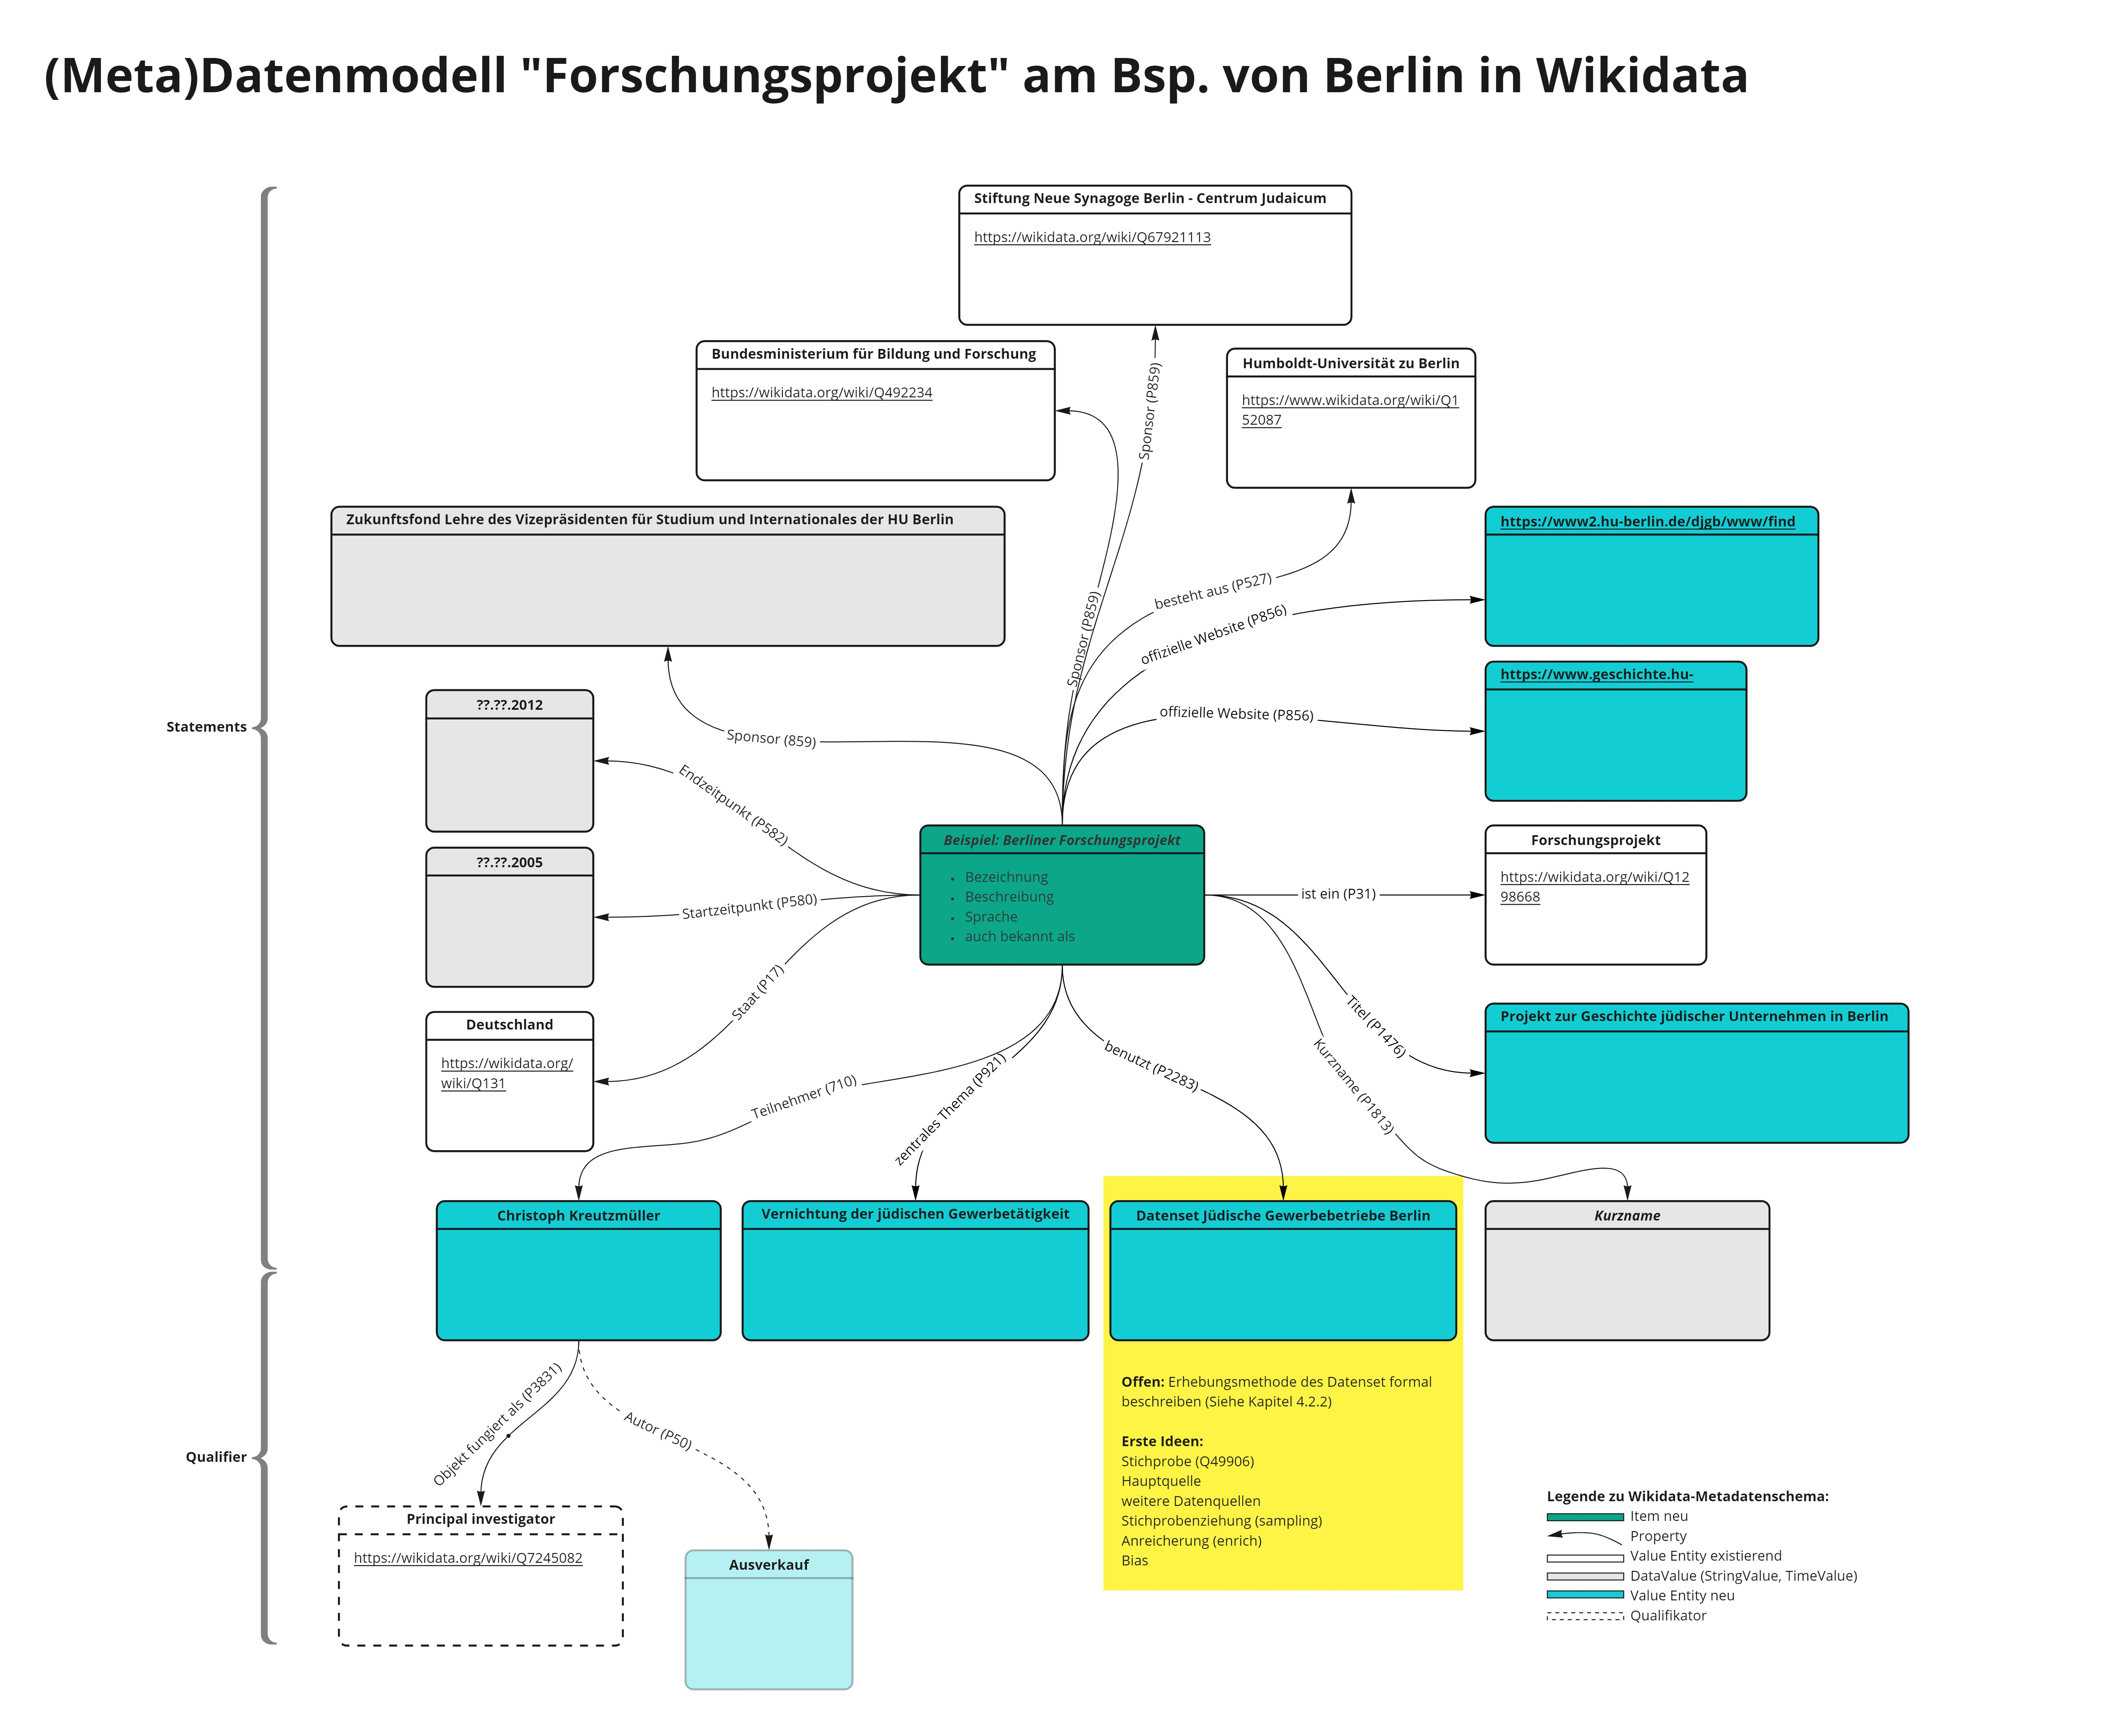
\includegraphics[width=\ScaleIfNeeded]{wikidata-item_research-project}}
    \caption{Modellierung der Forschungsprojekte in Wikidata.}
    \label{fig:x cubed graph} \footnotetext{Größere Darstellungen der Modellabbildungen sind alle separat nochmals im Anhang beigefügt.}
\end{figure}

Folglich wäre die eigene Modellierung von ,,Forschungsprojekt'' für die lokalen Forschungsprojekte im Forschungsfeld redundant, da diese von dem bestehenden Wikidata-Projekt abgeleitet werden kann (Abbildung 4.1).\footnote{Als Orientierung diente das Forschungsprojekt ,,Amyloid fibril cytotoxicity: new insights from novel approaches'', URL: \url{https://www.wikidata.org/w/index.php?title=Q52268104&oldid=1528020632}.} Aus dem Modell in Abbildung 4.1 geht darüber hinaus hervor, dass viele Entitäten in Wikidata bereits existieren und nicht neu angelegt werden müssen.\footnote{Entitäten mit weißem Hintergrund.} Auch die Verknüpfung von externen Information ist möglich. Die Deutsche Forschungsgemeinschaft (DFG) hat mit dem Informationssystem ,,GEPRIS – Geförderte Projekte der DFG'' (GEPRIS)\footnote{URL: \url{https://gepris.dfg.de/gepris/OCTOPUS?task=showAbout} (letzter Zugriff am 21.05.2022).} in Auszügen ihre Daten zu allen gegenwärtigen und vergangenen geförderten Projekten veröffentlicht. Dort ist auch das Forschungsprojekt ,,Geschichte mittlerer und kleiner jüdischer Unternehmen in Frankfurt am Main und Breslau 1929/39 bis 1945'' archiviert.\footnote{URL: \url{https://gepris.dfg.de/gepris/projekt/48308995?context=projekt&task=showDetail&id=48308995&} (letzter Zugriff am 23.05.2022). Hieraus ging u.a. die Lokalstudie zu Frankfurt am Main hervor sowie die im Interview erwähnte Access-Datenbank mit ca. 3.000 Gewerbebetrieben in Frankfurt a.M., Siehe Nietzel 2012 und Interview B2\_Transkript, Pos. 27.} Mit der vorhandenen Wikidata-Property ,,GEPRIS ID (Projekt) (P4870)'', kann demnach das DFG-Projekt mit dessen eindeutiger nummerischer DFG-Kennung ,,48308995'' in Wikidata verknüpft werden.\footnote{Auch die Freie Universität Berlin führt ein zentrales Projektverzeichnis mit detaillierten Informationen zu den einzelnen Projekten, siehe URL: \url{https://research.zuv.fu-berlin.de/projects} (letzter Zugriff am 24.05.2022).}  

Zusammengefasst bietet die vielfältige Nutzung der Wikidata eine Menge Nachnutzungsmöglichkeiten auch für die historische Forschung. Diese Form der Nachnutzung trägt außerdem zur Qualitätsicherung in Wikidata bei. Zudem können erstmals Projekt-Daten aus vrteilten Datenquellen in Wikidata zusammengeführt und auf diese Weise Informationen vernetzt werden. Sollten für das Forschungsfeld weitere Informationen notwendig werden, können diese dynamisch ergänzt werden, was wiederum der Vorteil des Linked Data-Konzept gegenüber einer herkömmlichen relationen Modellierung in einer SQL-Datenbank ist. Dort ist diese Flexibilität nicht gegeben. Dadurch, dass die Forschungsprojekte als eigene Wikidata-Items nun einen eindeutigen Wikidata-Identifikator besitzen, können sie den zugehörigen Forschungsdaten zugeordnet werden, womit der projektbezogene Entstehungsrahmen erstmals transparent wird.

\subsection{Erhebungsmethode}

Da die methodischen Vorgehensweisen der verschiedenen Wissenschaftsdisziplinen voneinander abweichen, existieren zu deren formalen Beschreibung keine disziplinübergreifenden Metadatenstandards.\footnote{Vgl. forschungsdaten.info, URL: \url{https://www.forschungsdaten.info/themen/beschreiben-und-dokumentieren/metadaten-und-metadatenstandards/} (letzter Zugriff am 15.05.2022).} Das heißt, diese als Prozessmetadaten bezeichneten Daten sind fachspezifisch. Im naturwissenschaftlichen Bereich und in der Archäologie gibt es mit der \textit{Research Resource Identification Initiative} (RRI)\footnote{} und mit \textit{IANUS}\footnote{URL: \url{https://ianus-fdz.de/}. Der Support war nach Auslaufen der DFG-Projektförderung 2017 allerdings eingeschränkt. So konnten neue Datensammlungen bis 2022 nicht aufgenommen werden, siehe URL: \url{http://datenportal.ianus-fdz.de/pages/information.jsp\#dateneigentuemer} (alle letzter Zugriff 15.05.2022).} bereits zentrale Ansätze, wie Methodiken schematisch und anhand von Thesauri oder festen Vokabularen formal beschrieben werden können.\footnote{Siehe zum Beispiel die Thesauri des Deutschen Archäologischen Instituts, URL: \url{http://thesauri.dainst.org/de.html} mit der Kollektion zu den Methoden, URL: \url{http://thesauri.dainst.org/de/collections/\_203bcc05.html} (alle letzter Zugriff am 15.05.2022).} Allerdings sind sie nicht übertragbar auf den geschichtswissenschaftlichen Bereich. Offenes Forschungsdatenmanagement ist hier mit zwei Herausforderungen konfrontiert. Erstens gibt es einen fachspezifischen Standard für die Geschichtswissenschaften nicht. Zweitens ist fraglich, wie sich die Erhebungsmethoden im Forschungsfeld formalisieren lassen. Als Einstiegspunkt soll hier der Versuch einer groben Schematisierung der methodischen Vorgehensweise anhand der Lokalstudien, welche systematisch Daten zu jüdischen Gewerbebetrieben erhoben haben, vorgenommen werden.\footnote{Das sind zuvorderst die Studien zu Hamburg, Berlin, Frankfurt am Main, München, Mannheim und Krefeld.} Zunächst ist festzuhalten, dass die Datenanalyse und -auswertung aller Studien auf Stichprobenziehung beruhte.\footnote{Interessant ist, dass alle Studien mit dem Anspruch gestartet sind, die Gesamtzahl jüdischer Gewerbetriebe zu erfassen. Dieser war allerdings von keiner Studie einlösbar, da erstens das Ausmaß der Zerstörung unterschätzt wurde und zweitens die Projektlaufzeit für eine Totalerhebung zu kurz war, vgl. Interview B3\_Transkript, Pos. 11 und B2\_Transkript, Pos. 23.} Festzustellen ist weiterhin, dass die Überlieferung überall als disparat und lückenhaft bezeichnet wurde, da viele Bestände teilweise oder überwiegend von den Nationalsozialisten vernichtet wurden, um Spuren zu verwischen, oder in den letzten Kriegstagen unwiederbringlich zerstört wurden. Oft sind nur Überreste und Splitter erhalten. Abbildung 4.2 zeigt einen idealtypischen Ablauf der Datenerhebung im Forschungsfeld. Demnach wurde eine Hauptquelle (Datenquelle 1) ausgewählt, aus der ein Sample gezogen wurde.\footnote{In München wurde jeder zweite Buchstabe aus der Gewerbekartei mit jüdischen Gewerbebetrieben erfasst, also ca. die Hälfte der Gewerbebetriebe, vgl. Rappl 2000, S. 179 Fußnote 217. In Frankfurt diente ebenfalls der Bestand aus dem Gewerbeamt als Hauptquelle (vgl. Interview B2\_Transkript, Pos. 31 und 45.), während in Mannheim das Verzeichnis jüdischer Gewerbetreibender sowie alle Arisierungsakten ab 1938 erhalten ist, vgl. Interview B3\_Transkript, Pos. 43 und 47 erhalten sind. In Hamburg basierte die Stichprobenziehung im Wesentlichen auf den Wiedergutmachungsakten, vgl. Bajohr 1998, S. 21ff. und Interview B1\_Transkript, Pos. 33.} In den meisten Fällen konnten daraus die wesentlichen Grunddaten (Name, Inhaber, Branche und Adresse) der Gewerbebetriebe erfasst. Ausgangspunkt bildeten im Idealfall publizierte und unpublizierte Verzeichnisse, Listen oder Karteisammlungen in denen Gewerbebetriebe dezidiert und systematisch mit dem Ziel der Verfolgung als jüdisch markiert und gelistet wurden.\footnote{In München übernahm diese Aufgabe das städtische Gewerbeamt, vgl. Rappl 2000, S. 145f. In Frankfurt am Main war der zentrale Akteur die Industrie- und Handelskammer.} Im nächsten Schritt wurden diese Daten mit weiteren Quellen abgeglichen, die den Vorgang der Verfolgung der einzelnen Gewerbebetriebe verwaltungsseitig dokumentierten. Zu dieser zweiten Datenquelle gehören verschiedene zeitgenössische Aktenbestände.\footnote{Zum Beispiel die Handelsregisterakten, die sogenannten Entjudungsakten oder die Akten der Devisenstellen, aber auch die Wiedergutmachungsakten nach 1945.} Aus diesem Rahmen fällt das Berliner Forschungsprojekt, wo man einen gänzlich anderen Ansatz verfolgt hat. Mangels überlieferter Quellen, wurde ein Sample anhand der Zentralhandelsregisterbeilage (ZHRB) erstellt und aus dieser die Aktivitäten aller handelsregisterlich geführten Unternehmen zwischen 1932 und 1942 erfasst. Man nahm hier folglich eine Gesamtaufnahme des Handelsregisters vor, welches im zweiten Schritt nacheinander mit weiteren Quellen abgeglichen und bei einer eindeutigen Indizienlage Gewerbebetriebe als jüdisch identifiziert wurden.\footnote{Der Autor beschreibt dieses unkonventionelle Vorgehen im Forschungsfeld sehr detailliert in der Einleitung seiner Studie, vgl. Kreutzmüller 2012, S. 29-38.} Auch wenn mit ca. 8.000 identifizierten jüdischen Gewerbebetrieben nur etwa 16 Prozenzt der insgesamt in Berlin ansässigen jüdischen Gewerbebtriebe erhoben werden konnte, stellt das Sample in Bezug auf das Handelsregister als Grundgesamtheit fast eine Vollerhebung dar.\footnote{Von der Forschung wird geschätzt, dass in Berlin rund die Hälfte der jüdischen Gewerbebetriebe im Deutschen Reich ansässig war, also rund 50.000. Kreutzmüller geht von ca. 10.000 im Handelsregister eingetragenen jüdischen Gewerbebetrieben aus, vgl. Kreutzmüller 2012, S. 102f.}

\begin{figure}[h]
    \centering
    \frame{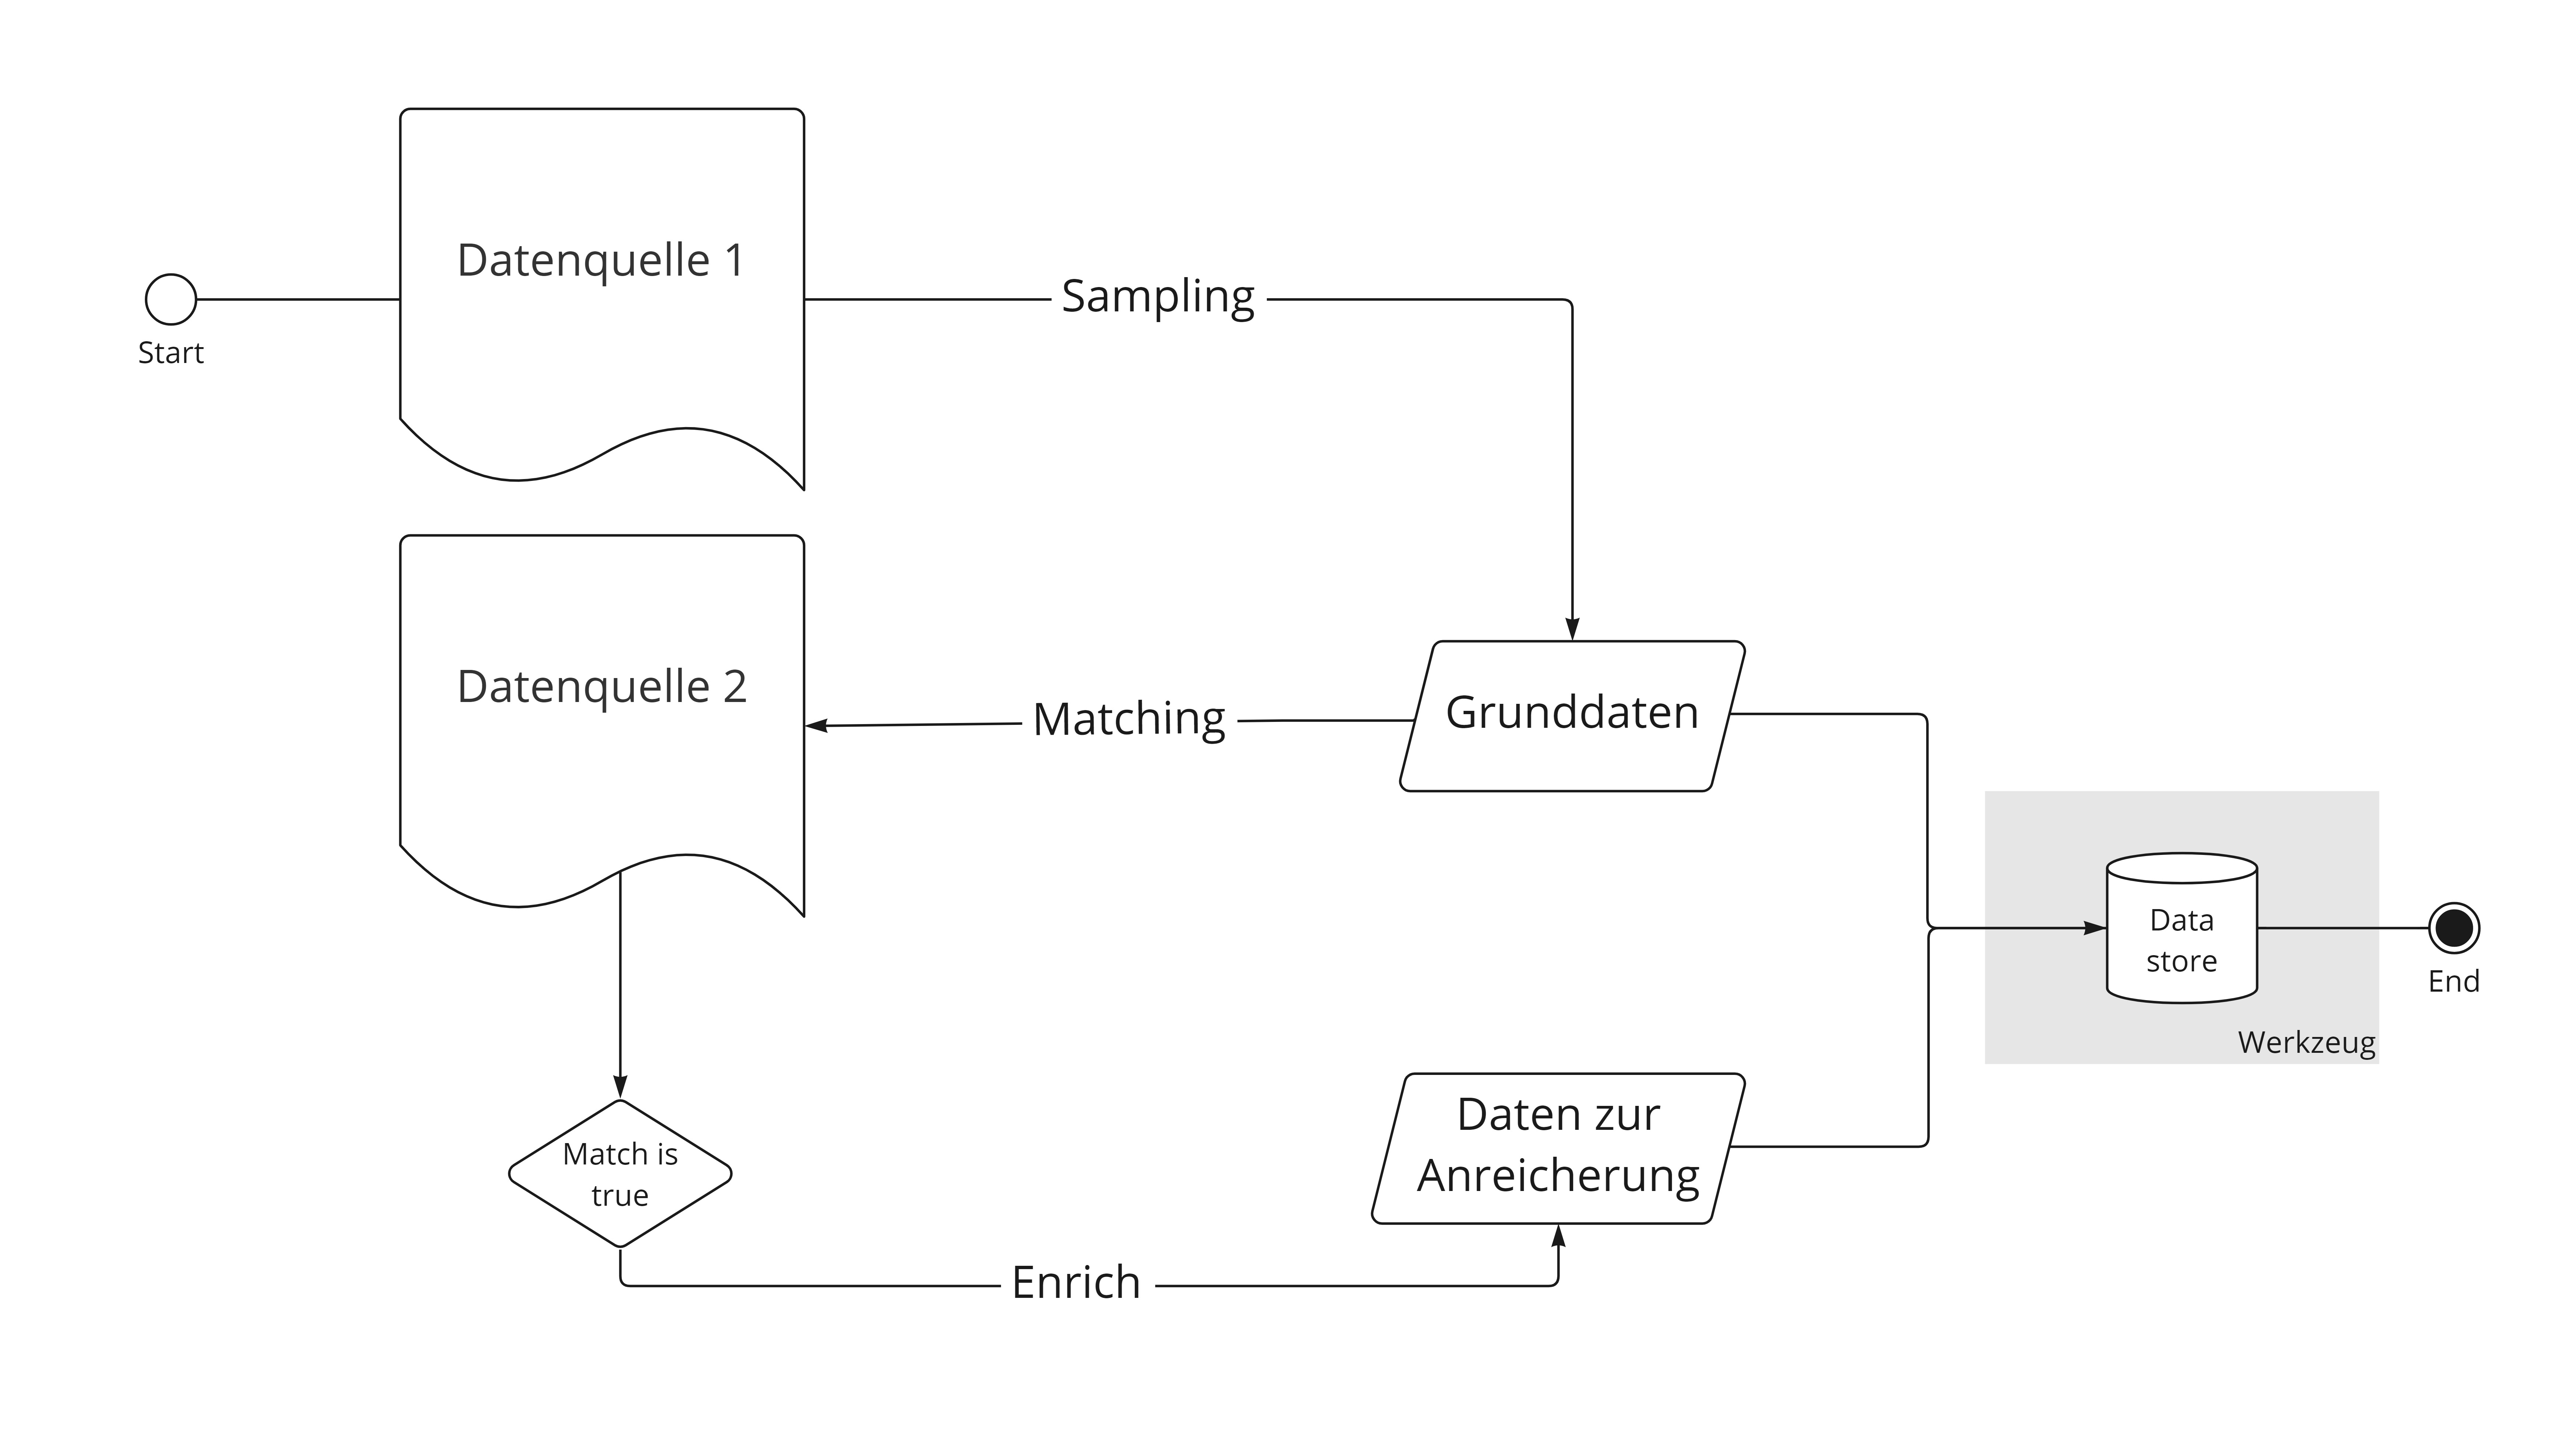
\includegraphics[width=\ScaleIfNeeded]{flowchart_data-collection}}
    \caption{Idealtypische Stichprobenziehung von Daten zu jüdischen Gewerbebetrieben.}
    \label{fig:x cubed graph}
\end{figure}

Nachteil der vereinfachten, groben Schematisierung ist, dass diese Detailinformationen nicht enthalten sind. Darüber hinaus fehlen die mit der Quellenlage einhergehenden Stichproben-Verzerrungen (Bias) der Studien, welche bisher überhaupt nicht kommuniziert werden:

\begin{itemize}
    \item Viele Hauptquellen setzen zeitlich erst mit den reichsweiten Gesetzen ab 1938 ein. Die frühe Phase der Vernichtung der jüdischen Gewerbetätigkeit bleibt somit unterrepräsentiert, weil schlichtweg Daten dazu fehlen.
    \item Bei der Verwendung von überwiegend Wiedergutmachungsakten, insbesondere aus Rückerstattungsverfahren wie in Hamburg, liegt der Schwerpunkt automatisch auf den größeren Unternehmensverkäufen und den ehemaligen Eigentümern, die den Nationalsozialismus meist durch Emigration überlebt haben. Liquidationen bleiben in diesem Ansatz unterrepräsentiert sowie der komplette Ostteil Deutschlands, da hier die Wiedergutmachung erst in den 90er Jahren mit dem Ende der DDR teilweise einsetzte.
    \item In Berlin wiederum liegt der Fokus mit der ZHRB auf den handelsregisterlich eingetragenen Firmen und damit auf mittelständischen Gewerbebetrieben, wodurch vor allem Kleinstunternehmen unterrepräsentiert bleiben. Außerdem liegt der Schwerpunkt auf Liquidationen, da das Handelsregister Besitzübernahmen nicht abbildet.
\end{itemize}

Es wird deutlich, dass geschichtswissenschaftliche Datenerhebungsmethoden aufgrund der historischen Quellengrundlage nicht analog zu den naturwissenschaftlichen Methoden standardisiert werden können. Es ist die Lückenhaftigkeit und es sind die Fehlstellen in der historischen Forschung, die eine adäquate Abbildung auf ein festes Schema zu einer spezifischen Herausforderung im Fach machen. Daher stellt sich insbesondere auch die Frage, welche Notwendigkeit Standardisierung hier besitzt. Es wäre genauer zu untersuchen, was der Mehrwert davon für die historische Forschung wäre oder ob zum Zwecke der methodischen Transparenz und Nachvollziehbarkeit eine rein textuelle Beschreibung oder Dokumentation zum Beispiel in Form einer Readme-Datei ausreicht. Tatsache ist, dass die Ausführungen zur Erhebung in die einzelnen Lokalstudien bisher unterschiedlich ausfallen und entscheidenden Informationen zum Verständnis der Forschungsdaten ganz fehlen. Auch im Sinne der Nachnutzbarkeit von historischen Forschungsdaten ist also die offene Frage, welche Informationen zur Methodik überhaupt benötigt werden.

\subsection{Problem \textit{Jüdischer} Gewerbebetrieb}

Da Untersuchungsgegenstand aller Lokalstudien ,,Jüdische Gewerbebetriebe'' oder ,,Jüdische Unternehmen'' sind, wurde folglich Daten zu jüdischen Gewerbebetrieben erfasst. Hieraus ergibt sich eine grundlegende methodische Schwierigkeit: Da die Konfessionszugehörigkeit bezüglich eines Gewerbebetriebs oder Unternehmens schlichtweg unlogisch ist, ist der Begiff alleine ohne Kontext unbrauchbar. Dieses Problem wird von dem meisten Studien reflektiert und betont, dass es sich hierbei um eine antisemitische Zuschreibung und Konstruktion handelte. Diese Kennzeichnung und Diffamierung diente den Nationalsozialisten als Instrument für die weiteren Verfolgungspraktiken. Zur einfacheren Handhabung wurde der Begriff als Quellenbegriff jedoch von allen Studien beibehalten. Hierbei fallen zwei unterschiedliche Verwendungen auf: 

\begin{itemize}
    \item Der Begriff ,,jüdischer Gewerbebetrieb'' wird ausschließlich auf die jüdischen Besitzer*innnen bezogen und angewandt.\footnote{Vgl. Janetzko 2012, S. 18.} Damit wird jedoch das methodische Problem nicht aufgelöst, sondern verlagert sich auf den Begriff ,,jüdische Person'' oder ,,Jude/ Jüdin'', bei dem es sich ebenfalls um eine rassistische Zuschreibung handelte und nichts mit dem Selbstverständnis der Betroffenen zu tun hatte.\footnote{Das wird in der Studie zu Hamburg auch ausführlich reflektiert. Vgl. Bajohr 1997, S. 9.} Darüber hinaus werden in dieser Verwendung weitere Verfolgungskontexte vernachlässigt. So war es in der frühen Phase der Verfolgung durchaus möglich, dass Gewerbebetriebe als jüdisch diffamiert wurden, die zum Beispiel einen hohen Anteil jüdischer Mitarbeiter*innen aufwiesen, deren Besitzer aber selbst nach der nationalsozialistischen Ideologie nichtjüdisch waren.\footnote{An diesem Beispiel zeigt sich überdies die in Wechselbeziehung stehenden Teilprozesse der Verdrängung der Juden aus dem Berufsleben und der Vernichtung der jüdischen Gewerbetätig deutlich.}
    \item Der Begriff ,,jüdischer Gewerbebetrieb'' wird mit ,,als jüdisch betrachtet/ verfolgt'' übersetzt. In dieser Verwendung ist die jüdische Eigentümerschaft eines Gewerbebetriebs zunächst unerheblich, das heißt sie wird nicht vorausgesetzt, sondern es werden alle Gewerbebetriebe erfasst, die im nationalsozialistischen Kontext diffamiert wurden. Damit wird einerseits der Konstruktioncharakter des Begriff hervorgehoben und andererseits dem Umstand Rechnung getragen, dass die rassistischen Zuschreibungen grundsätzlich jeglicher rationalen Begründung entbehrten und aus diesem Grund willkürlich erfolgen konnten.
\end{itemize}

Auch wenn in allen Studien der selbe Untersuchungsgegenstand genannt wird, so zeigt sich erst in der konkreten Verwendung, dass dieser unterschiedlich ausgedehnt werden konnte, weil der Begriff an sich nicht widerspruchsfrei ist. Aus forschungsethischer Perspektive ist zudem problematisch, dass ein rassistisch konnotierter Begriff in der wissenschaftlichen Forschung beibehalten wird. Wichtig wäre, sich im Forschungsfeld auf eine einheitliche Verwendung zu einigen, denn bisher werden Jüdische Gewerbebetrieben unterschiedlich erhoben. Hierzu wird keine abschließende Entscheidung getroffen, da dies in einem Diskurs im Forschungsfeld gemeinsam entschieden werden sollte. Um dafür den Anstoß zu geben und um insbesondere auch die forschungsethischen Implikationen kritisch zu reflektieren, wurde im erstellten Wikidata-Projekt\footnote{Zum Wikidata-Projekt siehe Kapitel 4.3.} der \textit{Wikidata talk} ,,How do we use and model ,Jüdischer Gewerbebetrieb'?'' mit der Disskussionsfunktion angelegt und zwei Vorschläge unterbreitet (Abbildung ): 

\begin{itemize}
    \item ,,Jüdischer Gewerbebetrieb'' wird als eigenes Item angelegt und mit Statements angereichert, die die nationalsozialistische Herkunft deutlich machen. Da in Wikidata Items von jedem/ jeder ohne Einschränkung angelegt werden können, wäre diese Lösung schnell umsetzbar. Bei der Frage mit welcher Eigenschaft (Property) das Item als Value auf einen Gewerbebetrieb abgebildet werden soll, lohnt abermals ein Blick auf benachbarte Wikidata-Projekte. Im Projekt \textit{Wikidata:WikiProject Victims of National Socialism} wurde 2020 die Verwendung des Begriffs ,,Holocaust-Opfer'' diskutiert.\footnote{Wikidata Talk:Q2763 (2020), Modeling of holocaust victim, URL: \url{https://www.wikidata.org/w/index.php?title=Talk:Q2763&oldid=1392179230}}. Da in der Wikidata Konvention ist, Personen so neutral wie möglich zu beschreiben und Zuschreibungen von außen mit entsprechenden Aussagen kenntlich zu machen, hat man sich im Wikidata-Projekt darauf geeinigt, den Begriff nunmehr zusammen mit ,,Subjekt fungiert als (P2868) Opfer des Holocaust (Q5883980)'' zu verwenden und nicht mehr als ,,ist ein(e) (P31) Holocaust-Opfer (Q5883980)''.\footnote{Siehe zum Beispiel Wikidata-Item Anne Frank (Q4583), URL: \url{https://www.wikidata.org/w/index.php?title=Q4583&oldid=1645273699}.} Diese Verwendung kann für Gewerbebetriebe übernommen werden. Zwar geht es hier ausdrücklich nicht um Personen. Da aber die Verwendung ,,ist ein(e) (P31) Jüdischer Gewerbebetrieb (Q???)'' - wie gezeigt wurde - unlogisch wäre, bietet sich ,,Subjekt fungiert als (P2868) Jüdischer Gewerbebetrieb (Q???)'' an.
    \item Statt als Item kann ,,Jüdischer Gewerbebetrieb'' auch als Property ,,als jüdisch betrachtet/ verfolgt (P???)'' oder ähnlich modelliert werden.\footnote{Dieser Ansatz wurde vom Berliner Forschungsprojekt umgesetzt.} Da diese Eigenschaft bisher noch nicht existiert, wäre diese Umsetzung etwas langwieriger, da Eigenschaften in der Wikidata nicht von jedem/jeder erstellt werden, sondern zunächst vorgeschlagen werden müssen.\footnote{Wikidata:Eigenschaften vorschlagen (2022), URL (stable): \url{https://www.wikidata.org/w/index.php?title=Wikidata:Property_proposal/de&oldid=1624532274}.} Nach einer öffentlichen Debatte entscheidet eine berechtigte Administratoren-Gruppe der Wikidata, ob die Property neu aufgenommen wird oder ob Alternativ-Eigenschaften zur Verfügung stehen. Mit diesem Verfahren sollen Redundanzen und Widersprüchlichkeiten verhindert werden. Es dient zur Qualitätskontrolle der Wikidata. Daher ist es möglich, dass für das Forschungsfeld notwendige Eigenschaften für die Wikidata insgesamt nicht die Relevanz besitzen und aus diesem Grund abgelehnt werden können. Wie liberal oder konservativ die Wikidata-Politik hier ist, müsste erprobt werden.      
\end{itemize} 

\begin{figure}[h]
    \centering
    \frame{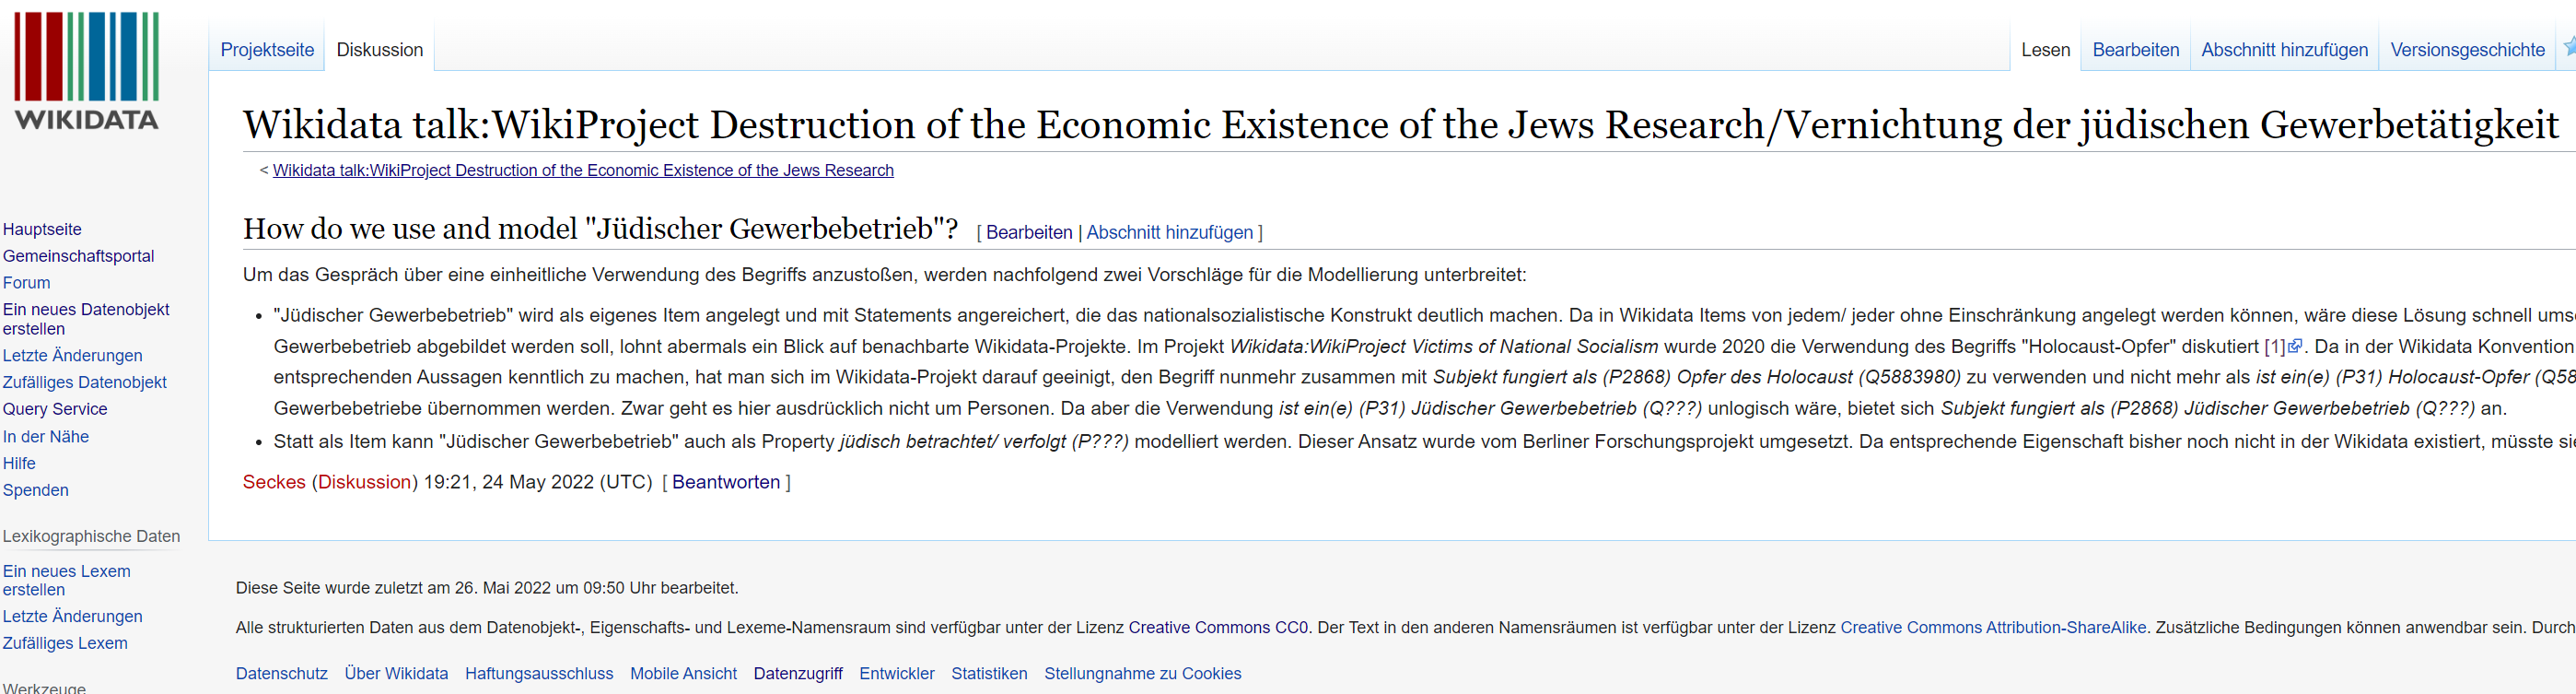
\includegraphics[width=\ScaleIfNeeded]{wikidata-discussion-jued-gewerbebetrieb}}
    \caption{Diskussionsseite zur Frage, wie "Jüdischer Gewerbebetrieb" verwendet und modelliert werden soll.}
    \label{fig:x cubed graph}
\end{figure}

\section{Aufbereitung}

\begin{quote}
    Also ich denke, die sitzen alle auf irgendwelchen Excellisten oder wenn das ältere Forschungsprojekte sind, Herr Bajohr weiß ich nicht, ob der schon Excel genutzt hat für sein Hamburg-Buch oder ob der noch Karteikarten hatte.\footnote{Interview B3\_Transkript, Pos. 79.}
\end{quote}

Um eine valide Datengrundlage für die Analyse zu erhalten, werden die erhobenen Rohdaten vorab aufbereitet. Damit erfolgt erstmalig eine Verarbeitung der Daten, denn der Operationalisierung der Forschungsfragen entsprechend werden die Daten ausgewählt, strukturiert erfasst und bereinigt. In der historischen Forschung liegt die Situation vor, dass die Rohdaten im Quellenmaterial bereits vorliegen, sich aber mitunter über viele Quellen verteilen. Daher muss festgelegt werden, erstens welche Informationen aus den Quellen extrahiert werden sowie zweitens, mit welchem Werkzeug diese strukturiert und organisiert werden sollen. Dieser Prozess der Forschungsdaten-Genese ist bisher im Forschungsfeld weitestgehend unsichtbar und findet lediglich in den Studien zu Berlin und Frankfurt am Main nachträglich in den Publikationen Erwähnung.\footnote{Vgl. Kreutzmüller 2012, S. 38f., Nietzel 2012, S. 17.}. In beiden Projekten kamen ,,Datenbanken'' zum Einsatz, die anhand der Interviews als Microsoft Access-Datenbanken der Version 2007 spezifiziert werden konnten.\footnote{Vgl. Interview B2\_Transkript, Pos. 27.} Da es sich hierbei um eine Anwendung handelt, deren Datenorganisation auf relationalen Tabellen beruht, braucht es als Basis vorab ein Datenmodell, visualisiert zum Beispiel anhand eines Entity-Relationship-Diagramms (ERD) mit einer Beschreibung der darin verwendeten Elemente. Dieses ist für beide Studien allerdings nicht verfügbar. Damit ist eine Beurteilung der Daten hinsichtlich ihrer Verarbeitung bisher nicht möglich. Ziel von offenem Forschungsdatenmanagement ist es, die bisher unsichtbare Phase der Aufbereitung durch kollaborative Zusammenarbeit im Forschungsfeld transparenter zu gestalten. 

Zu diesem Zweck wurde in Wikidata das Projekt \textit{Wikidata:WikiProject Destruction of the Economic Existence of the Jews Research} erstellt (Abbildung 4.3.).\footnote{URL: \url{https://www.wikidata.org/wiki/Wikidata:WikiProject_Destruction_of_the_Economic_Existence_of_the_Jews_Research}.} Dieses besitzt grob drei Funktionen: Erstens können beliebig viele Seiten mithilfe von standardisierten Templates hierarchisch im Projekt angelegt werden (Pages und Subpages).\footnote{Siehe URL: \url{https://www.mediawiki.org/wiki/Help:Templates} (letzter Zugriff am 24.05.2022).} Diese bieten die Möglichkeit, die in Kapitel 3 methodisch aufgegriffene Taxonomie und damit die unterschiedlichen Zugänge im Forschungsfeld funktional umzusetzen. Auf der Hauptseite (Home) wurden bereits Hintergrundinformatioen zum Projekt sowie zu dessen Zielen hinzugefügt. Dort ist auch erwähnt, dass diese Arbeit nur den Ausgangspunkt bildet und von hier aus sukzessive die angrenzenden Untersuchungsbereiche integriert werden können. Außerdem findet sich hier die nicht unwichtige Information, dass die Taxonomie im Forschungsfeld dem Systematisierungversuch von Nietzel aus dem Jahr 2009 entlehnt ist.\footnote{Siehe Kapitel 3.2.1.}

\begin{figure}[h]
    \centering
    \frame{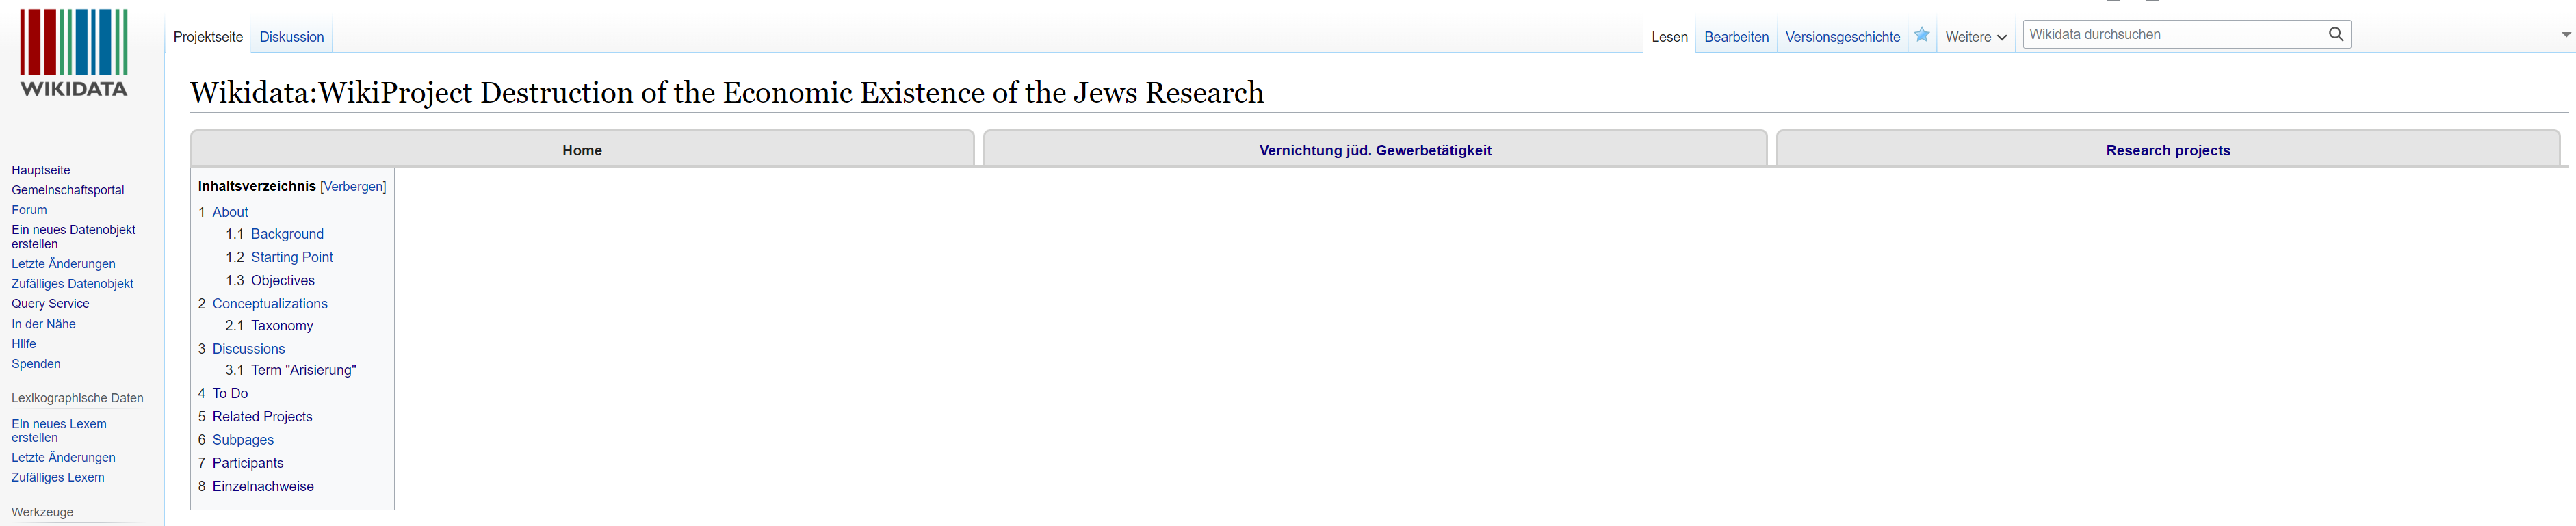
\includegraphics[width=\ScaleIfNeeded]{wikidata-project_tabs}}
    \caption{Wikidata:WikiProject Destruction of the Economic Existence of the Jews Research mit den in Tabs angelegten Subpages.}
    \label{fig:x cubed graph}
\end{figure}

Die bisherige Implementierung versteht sich explizit als Vorschlag, um eine Ausgangsbasis zu haben, von der aus Anpassungen und Weiterentwicklungen möglich werden. Um später in den gemeinsamen Austausch zu treten und Änderungen vorzunehmen, kann hierfür die zweite grundlegende Funktion der Diskussionseiten genutzt werden. Schließlich gibt es mit der Versionierung (,,Versionsgeschichte'') eine Kontrollfunktion, mit der sich alle Bearbeitungen zurückverfolgen und gegebenfalls auf einen früheren Stand zurücksetzen lassen.\footnote{URL: \url{https://www.wikidata.org/w/index.php?title=Wikidata:WikiProject_Destruction_of_the_Economic_Existence_of_the_Jews_Research&action=history} (letzter Zugriff am 24.05.2022).} Ingesamt bietet das Wikidata-Projekt damit die Möglichkeit des kollaborativen Austauschs und der gemeinsamen Strategieentwicklung im Forschungsfeld. Erstmals können Methodiken und Konzepte im Forschungsfeld diskutiert sowie in Bezug auf die in der Arbeit betrachteten Forschungsdaten ein allgemeingültiger Leitfaden zur Erfassung jüdischer Gewerbebetriebe entwickelt werden. Thematisch ist das Wikidata-Projekt in die Kategorien \textit{History WikiProjects} und \textit{Research WikiProjects} eingeordnet.\footnote{Siehe Wikidata:WikiProjekte, URL: \url{https://www.wikidata.org/wiki/Wikidata:WikiProjects/de} (letzter Zugriff am 24.05.2022).} Hier zeigt sich darüber hinaus, dass benachbarte Forschungsfelder zum Nationalsozialismus und zum Holocaust bereits mit eigenen Projekten vertreten sind, womit sich Anknüpfungspunkte über das Forschungsfeld hinaus ergeben.\footnote{Siehe WikiProject WWII, URL: \url{https://www.wikidata.org/wiki/Wikidata:WikiProject\_WWII}; WikiProject NS Perpetrator Research, URL: \url{https://www.wikidata.org/wiki/Wikidata:WikiProject\_NS\_Perpetrator\_Research}; WikiProject Victims of National Socialism, URL: \url{https://www.wikidata.org/wiki/Wikidata:WikiProject\_Victims\_of\_National\_Socialism}; WikiProject NS-Täterforschung, URL: \url{https://www.wikidata.org/wiki/Wikidata:WikiProject\_NS-Täterforschung}; Wikidata:WikiProject Nuremberg Trials, URL: \url{https://www.wikidata.org/wiki/Wikidata:WikiProject\_Nuremberg\_Trials} (alle letzter Zugriff am 24.05.2022).} 

\subsection{Zusammenführung der Quellen}

\paragraph{Datenmodell} Beim Zusammenführen der Quellen wurden die ausgewählten verteilten Informationen als strukturierte Daten zentral in Excel oder Access gespeichert. Auch wenn es in den Interviews von keinem Befragten bewusst formuliert wurde, so haben alle zur ,,Handhabbarmachung der Informationen''\footnote{Kreutzmüller 2012, S. 38.} eine \textit{Modellierung} von den zu erfassenden Daten vorgenommen. Bei diesem Vorgang wird ein eindeutig definierter realer Ausschnitt auf ein Modell abgebildet und die enthaltenen Konzepte operationalisiert. Aus den Interviews geht außerdem hervor, dass ein Datenmodell vorab nicht fest fixiert war, sondern dieses parallel zur Datenerfassung entstand und erweitert wurde.\footnote{Interview B1\_Transkript, Pos. 3, B2\_Transkript, Pos. 31 und Interview B1\_Transkript, Pos. 75.} Daraus ergeben sich zwei Anforderungen an offenes Forschungsdatenmanagement: Kollaborative Zusammenarbeit zwischen den Projekten kann nur funktionieren, wenn man sich auf eine Terminologie und auf ein Schema einigt. Es müssen folglich erstens die vielen unterschiedlichen Modelle und Begriffe der einzelnen Studien für eine gemeinsame Nutzung kompatibel gemacht werden. Da aufgrund der besonderen Überlieferungsstruktur ein statisches Modell vorab nicht feststeht, muss dieses zweitens dynamisch und skalierbar sein.

Anhand der für die Arbeit zu Verfügung gestellten Daten aus Berlin, Mannheim und Krefeld sowie mithilfe der Interviews wurde zunächst versucht, eine begriffliche Kontrolle im Untersuchungsfeld zur Vernichtung der jüdischen Gewerbetätigkeit im NS zu erhalten. Hierbei wurde sich der Methodik der Dokumentbeschreibungssprachen aus den Bibliotheks-, Dokumentations- und Informationswissenschaften bedient, mit der Fachgebiete mittels Thesauri oder Klassifikationen hierarchisch geordnet und inhaltlich erschlossen werden (Sacherschließung).\footnote{Siehe Gernot Wersig: Thesaurus-Leitfaden. Eine Einführung in das Thesaurus-Prinzip in Theorie und Praxis, Berlin, Boston 2016, doi:10.1515/9783111412719.} In diesem Sinne wird das Untersuchungsfeld als eigenes Begriffssystem verstanden, mittels dessen es sich inhaltlich beschreiben lässt.\footnote{Der erstellte Thesaurus als Anhang ... beigefügt.} Auf diese Weise konnte nicht nur eine Übersicht über die wesentlichen historischen Informationen im Untersuchungsfeld erstellt werden, sondern es zeigte sich mit dieser Methode auch, dass es zum einen Mehrdeutigkeiten bei der Bezeichnung von Sachverhalten gibt (Synonymproblem) und zum anderen Unklarheiten bestehen, wie Begriffe angewandt werden sollen.\footnote{Ebd., S. 47-51.} Für das Synonymproblem können Äquivalenzklassen vorgeschlagen werden.\footnote{Im Modell in den einzelnen Kästchen fett hervorgehoben} Die unklaren Begriffe müssen in dieser Arbeit offen bleiben, da abschließend deren globale Relevanz für das Forschungsfeld nicht bestimmt (z.B. Insolvenz)\footnote{Die Geschäftsauflösung bzw. Insolvenz wurde nur in der Krefelder Studie untersucht.} oder ihre Ambiguität (z.B. Geschäftsaufgabe) nicht aufgelöst werden konnte. 

Das feine Begriffssystem\footnote{Im Modell grau hinterlegt} wurde grob abstrahiert, sodass die generischen Begriffe auf der ersten Ebene eine Top-Level-Ontologie ergeben, die Studien-unabhängig auf alle Forschungsdaten im Forschungsfeld und darüber hinaus angewandt werden kann.\footnote{Siehe zu Top-Level-Ontologie Rehbein, Ontologien, 2017, S. 162-174.} Auf diese Weise kann das Datenmodell kompatibel und interoperabel gehalten werden, in der Konsequenz also zukünftig auch an andere Forschungsfelder anschließen.

Das generische Metadatenschema wurde im nächsten Schritt in das Wikidata-Projekt integriert, welches somit eine Strukturierung der Daten grob vorgibt (Abbildung 4.5.). 

\begin{figure}[h]
    \centering
    \frame{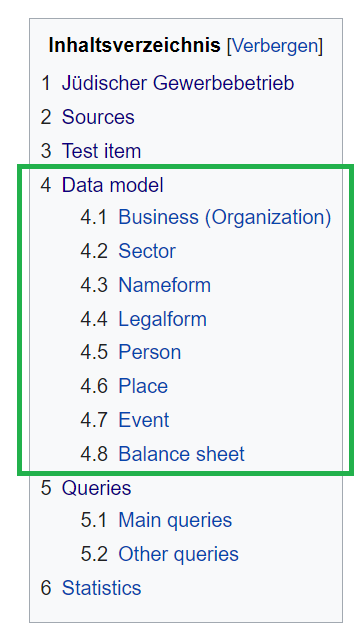
\includegraphics[scale=0.6]{wikidata-data-model-generic}}
    \caption{Integration des Metadatenschemas in Wikidata.}
    \label{fig:x cubed graph}
\end{figure}

Am Beispiel des Berliner Gewerbebetriebs ,,Gorbatschow Liköre F. Kramer \& Co'', welches 1938 vom Eigentümer Josef Kramer verkauft werden musste, wurde ein erster Entwurf für das präzise Datenmodell in Wikidata erstellt.\footnote{Das Modell ist als Anhang ... beigefügt.} Analog zur Modellierung der Forschungsprojekte wurden vorhandene Items und Properties nachgenutzt. Wo dies nicht möglich war, sind die Entities farblich markiert. Der Entwurf wurde anschließend im Wikidata-Projekt dokumentiert (Abbildung 4.6. Siehe auch Wikidata-Projekt, URL (stable): \url{https://www.wikidata.org/w/index.php?title=Wikidata:WikiProject\_Destruction\_of\_the\_Economic\_Existence\_of\_the\_Jews\_Research/Vernichtung\_der\_jüdischen\_Gewerbetätigkeit&oldid=1648462059}.).   

\begin{figure}[h]
    \centering
    \frame{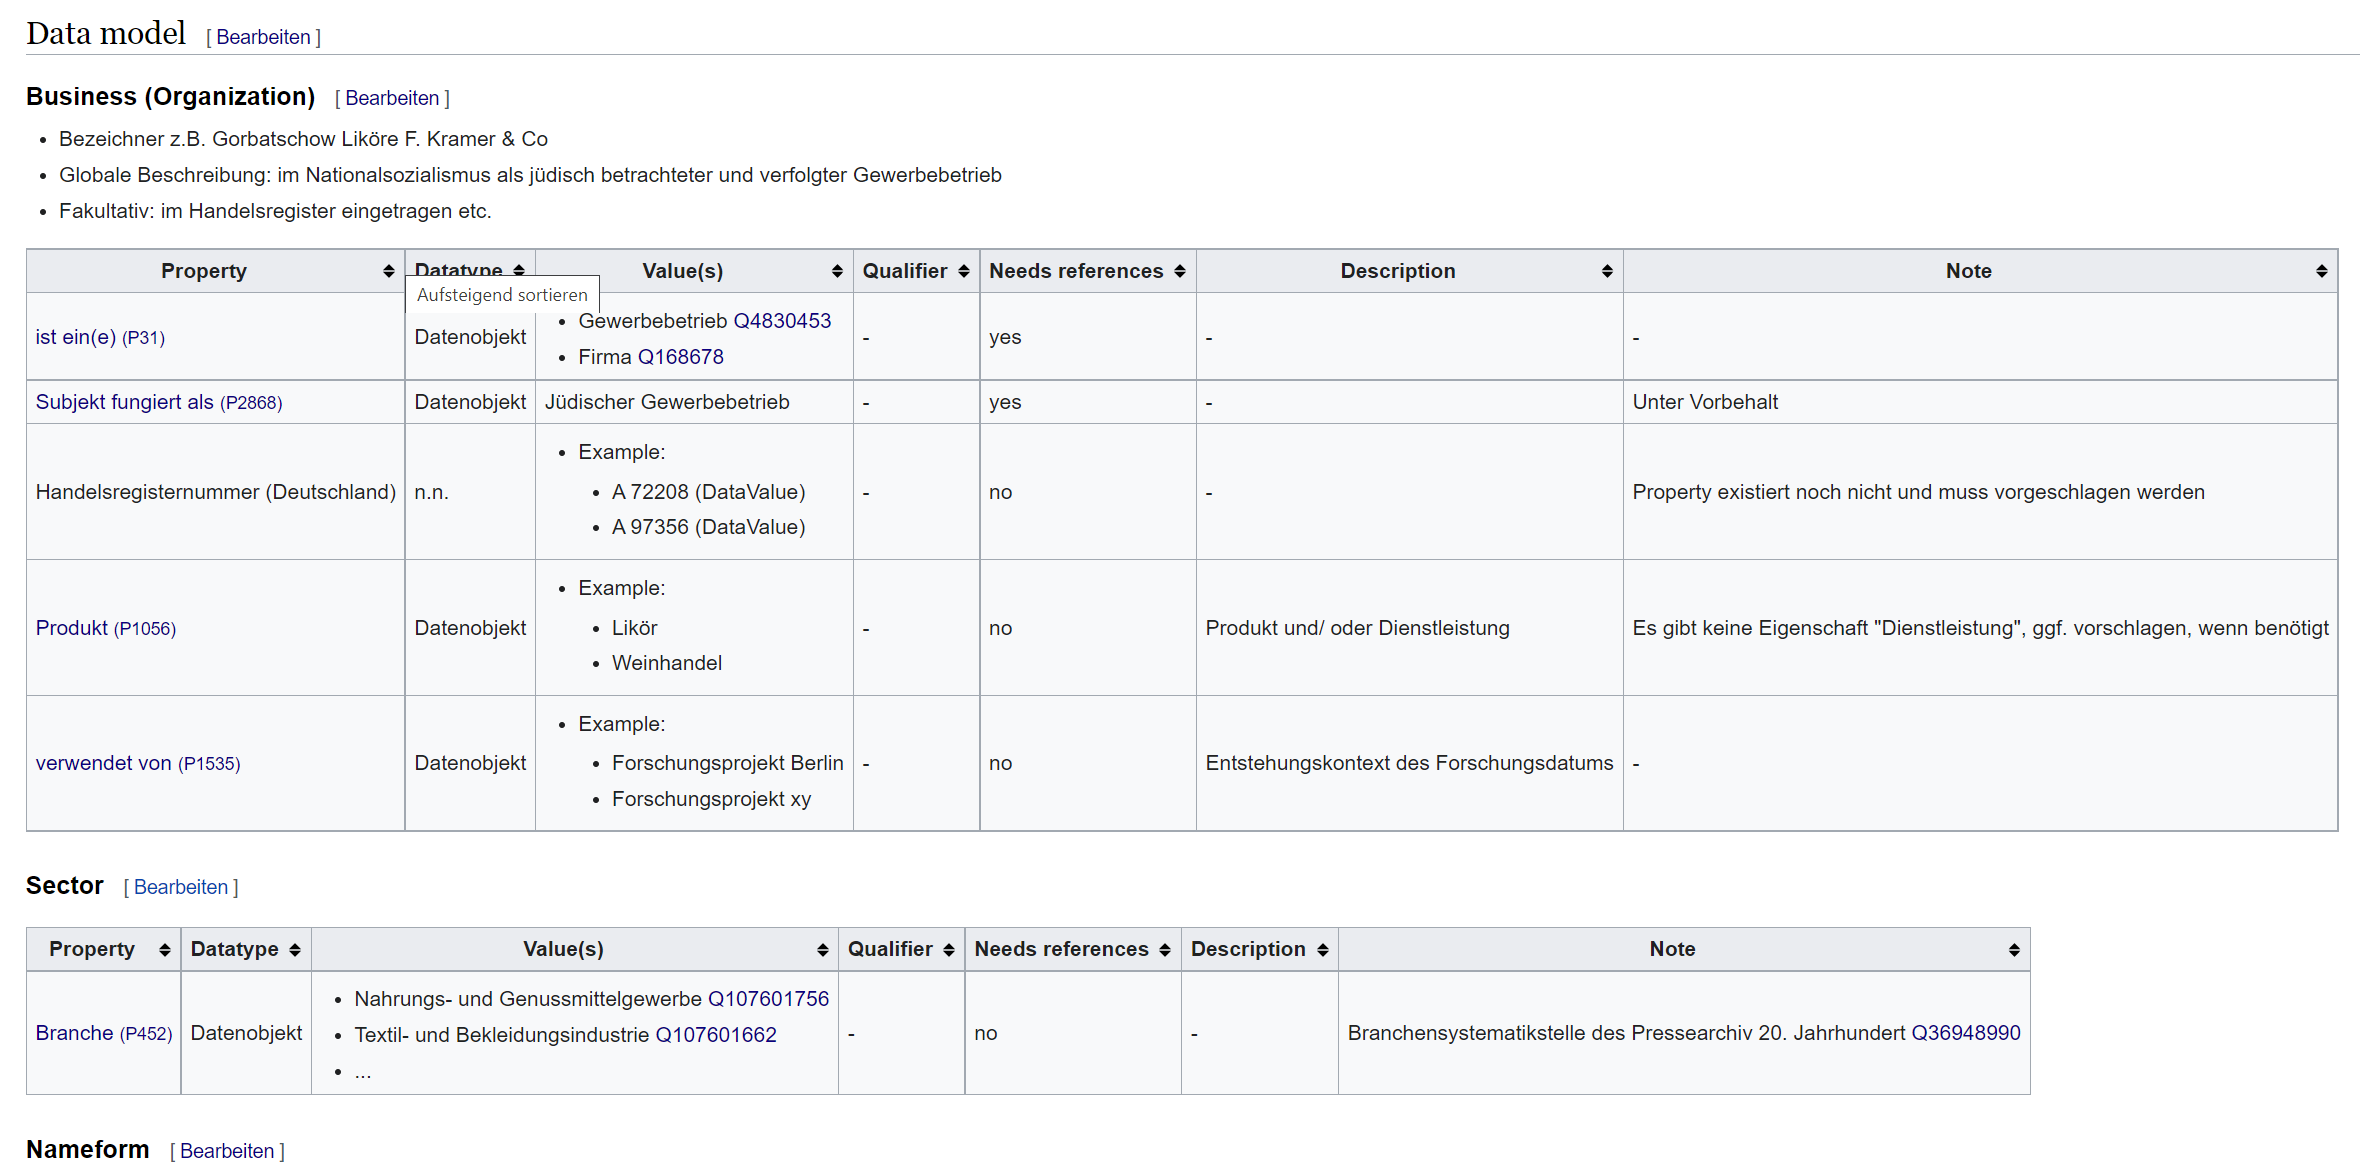
\includegraphics[width=\ScaleIfNeeded]{wikidata-data-model}}
    \caption{Beschreibung der Statements zu den einzelnen Entities.}
    \label{fig:x cubed graph}
\end{figure}

Hier kann das Datenmodell zur Beschreibung jüdischer Gewerbebetriebe kollaborativ angepasst und weiterentwickelt werden. In der Tabelle in Abbildung 4.6 stellt jede Zeile eine Aussage zu einer Entität dar (im Bild Gewerbebetrieb und Branche). In dieser können neben der Statements außerdem Verwendungsregeln und detaillierte Beschreibungen festgehalten werden. Das aktuelle prototypische Datenmodell versteht sich lediglich als Vorschlag und soll in erster Linie den Anstoß für weitere Diskussionen geben. Denn insbesondere die Frage nach der Modellierung der Forschungsdaten wird im Forschungsfeld bisher nicht systematisch bearbeitet. Aber schon in dieser frühen Phase ergeben sich Pfadabhängigkeiten, die Einfluss auf die anschließende Datenanalyse haben. Dies kann an einem Beispiel veranschaulicht werden: Wenn zu einem Gewerbebetrieb nur eine Adresse strukturiert erfasst wird (1:1 Kardinalität), können (überregionale) Umzüge später nicht mehr untersucht werden. In Berlin gab es in der Access-Datenbank nur Felder für eine Adresse pro Gewerbebetrieb. Weitere Adressen wurden unstrukturiert in sogenannten Freitextfeldern erfasst. Damit war und ist es nur schwer möglich, sich der Untersuchung von Ausweichsbewegungen - was in Berlin nur auf qualitativer Ebene geschah - quantitativ zu nähern.\footnote{siehe Kreutzmüller 2012, S. 310-310 (Kap. Umzug).} Wikidata mit dem dahinter stehenden Linked Data-Konzept bietet demgegenüber den entscheidenden Vorteil, dass ausschließlich strukturierte Daten in Subjekt-Prädikat-Objekt-Ausdrücken erfasst sowie neue Properties und Items dynamisch ergänzt werden können. Eine aufwändige Anpassung des Datenmodells entfällt dadurch. Die Einschränkung ist jedoch, dass erfasste Daten zu Jüdischen Gewerbebetrieben nicht gegen das Modell geprüft werden können. Das bedeutet, dass Daten auf der technischen Ebene auch dann gültig wären, wenn diese vollkommen anders erfasst würden. Damit ist eine Kontrolle über die Gültigkeit von Daten zu Jüdischen Gewerbebetrieben zum jetzigen Zeitpunkt nicht gegeben. Wikidata bietet aber mit dem Ziel der weiteren Qualitätssicherung die Erstellung von \textit{EntitySchemas} an (Abbildung 4.7).\footnote{Siehe Wikidata Schemas, URL: \url{https://www.wikidata.org/wiki/Wikidata:Schemas}. Siehe zum Beispiel das Entity Schema zu Mensch (E10), URL: \url{https://www.wikidata.org/wiki/EntitySchema:E10} (alle letzter Zugriff am 27.05.2022).} Damit ließe sich ein verbindliches Schema zur Erfassung von Jüdischen Gewerbebetrieben definieren. Dies ist jedoch erst dann sinnvoll, wenn ein gemeinsamer Grundstamm an Aussagen im Forschungsfeld feststeht.

\begin{figure}[h]
    \centering
    \frame{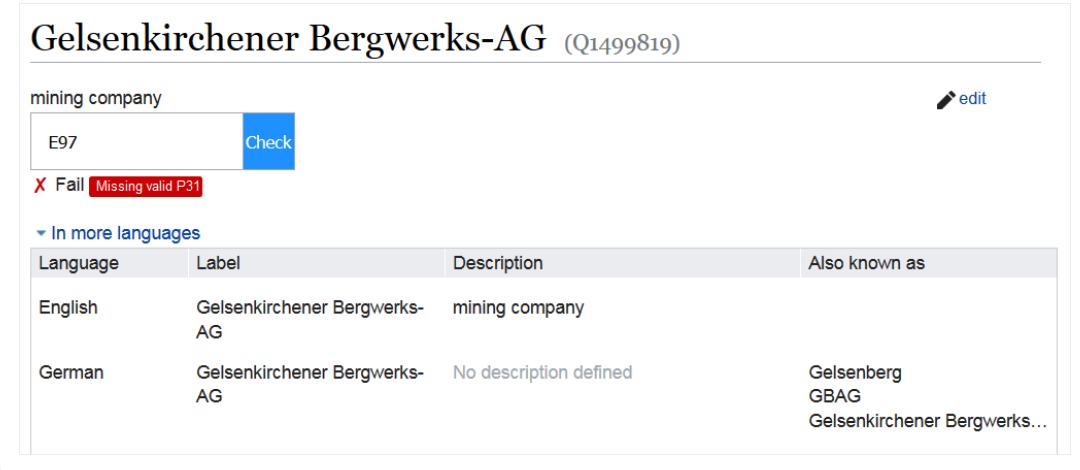
\includegraphics[scale=0.7]{wikidata-entity-schema}}
    \caption{Mithilfe von EntitySchemas können Daten gegen ein fest definiertes Schema auf ihre Gültigkeit hin geprüft werden.}
    \label{fig:x cubed graph}
\end{figure}

\paragraph{Personenbezogene Daten}

Auch wenn die Daten zu jüdischen Gewerbebetrieben größtenteils als ethisch unbedenklich eingestuft wurden\footnote{Vgl. Kapitel 3.5.}, gibt es mit den Unternehmenseigentümern personenbezogene Daten, die besondere forschungsethische Fragen aufwerfen, wenn sie in Open Data verfügbar sind. Zu beachten ist, dass es sich in der Regel nicht um Personen des öffentlichen Interesses handelt, was eine detaillierte Veröffentlichung bibliografischer Daten rechtfertigen würde. Das bedeutet, dass der Eigentümer Josef Kramer von Gorbatschow Liköre F. Kramer \& Co nicht mit Anne Frank\footnote{Wikidata-Item Anne Frank (Q4583), URL: \url{https://www.wikidata.org/wiki/Q4583}.} oder der Holocaust-Überlebenden und Aktivistin Margot Friedländer\footnote{Wikidata-Item Margot Friedländer (Q1895371), URL: \url{https://www.wikidata.org/wiki/Q1895371}.} gleichzusetzen ist. Gerade auch die Fälle, wo ehemalige Inhaber den Holocaust durch Emigration überlebt haben und nach 1945 einen Antrag auf Rückerstattung stellten, können rechtliche Einwände gegen eine Veröffentlichung von detaillierten personenbezogenen Daten sprechen.\footnote{Vgl. Kapitel 3.5.} Anders als bisher im Forschungsfeld braucht offenes Forschungdatenmanagent in Wikidata hier ein gemeinsames Vorgehen sowie eine klare und nachvollziehbare Strategie, die den verantwortungsvollen Umgang mit diesen sensiblen Daten sicherstellt. 

Hierzu wird folgende Empfehlung gemacht: Generell sollte das grundlose Sammeln personenbezogener Daten vermieden werden. Das bedeutet, auch wenn sie in den Quellen vorhanden sind, aber nicht der Bearbeitung von Forschungsfragen direkt dienen, werden sie nicht in Wikidata aufgenommen. Der Grundsatz ist, so wenig wie möglich personenbezogene Daten und so viel wie nötig zu erfassen. Sofern es also keine personenbezogenen Forschungsfragen gibt, werden lediglich Daten erfasst, die im Zusammenhang mit der unternehmerischen Tätigkeit stehen. Dies wurde am Beispiel der Gorbatschow Liköre F. Kramer \& Co für den Eigentümer Josef Kramer in Wikidata umgesetzt.\footnote{Wikidata-Item Josef Kramer (Q112135768), URL: \url{https://www.wikidata.org/wiki/Q112135768}.} Wenn wie in einigen Lokalstudien das Schicksal der Eigentümer nach der Besitzübernahme oder Liquidation statistisch untersucht werden soll\footnote{Siehe Bajohr 1998, S. 388 und Nietzel 2012, S. 121ff.}, werden hier nur die wesentlichen Informationen zu Emigration oder Deportation aufgenommen. Bei der Beschreibung des Verfolgungskontextes wird auf das bereits erwähnte WikiData-Projekt ,,Wikidata:WikiProject Victims of National Socialism'' zurückgegriffen. Demnach werden die Eigentümer*innen mit ,,Subjekt fungiert als (P2868) Holocaustüberlebender (Q12409870)'' bzw. ,,Subjekt fungiert als (P2868) Opfer des Holocaust (Q5883980)'' beschrieben. Für deren Schicksal werden die Aussagen ,,Schlüsselereignis (P793) ist ein(e) (P31) Holocaust-Gefangenentransport (Q61927259)'' bzw. ,,Schlüsselereignis (P793) ist ein(e) (P31) Auswanderung (Q187668)'' verwendet. Für den Fall, dass es weitere Informationen zu den Eigentümer*innen in externen öffentlichen Datenbanken gibt, die aber für die eigene Forschung nicht relevant sind, kann zur Datenvernetzung die eindeutige externe Personenkennung als Wikidata-Identifikator hinzugefügt werden (Abbildung 4.8).

\begin{figure}[h]
    \centering
    \frame{
\includegraphics[width=\ScaleIfNeeded]{wikidata-idenficator}}
    \caption{VIAF-Kennung der Holocaustüberlebender und Aktivistin Eva Schloss als Wikidata-Identifikator im zugehörigen Wikidata-Item \url{https://www.wikidata.org/wiki/Q90250}.}
    \label{fig:x cubed graph}
\end{figure}

Aus forschungsethischer Sicht kann das in dieser Arbeit angelegte Wikidata-Projekt ein Forum sein, wo die Handhabung personenbezogener Daten diskutiert werden kann und wo allgemeingültige Grundsätze sowie Strategien festgehalten werden können.\footnote{Der Vorschlag aus dieser Arbeit wurde auf der Diskussionsseite im Wikidata-Projekt dokumentiert.} Damit wäre es über die Datenmodellierung hinaus eine Plattform, die wichtige Orientierung im Umgang mit sensiblen Daten im Forschungsfeld gibt vor allem auch für Forscher*innen, die sich gänzlich neu mit dem Thema befassen.

\paragraph{Quellennachweise}

Die Information, woher die Daten zu jüdischen Gewerbebetrieben kommen, stellt das vielleicht wichtigste Qualitätskriterium von offenem Forschungsdatenmanagement im Forschungsfeld dar.\footnote{Vgl. Interview B1\_Transkript, Pos. 139 und Interveiw B3\_Transkript, Pos. 73.} Insbesondere weil der Untersuchungsgegenstand ,,Jüdischer Gewerbebetrieb'', wie gezeigt worden ist, methodische Schwierigkeiten mit sich bringt, braucht es Nachweise, die diesen in den Quellen eindeutig belegen. Wikidata ist für diese Anforderung funktional besonders gut geeignet. Denn die globale Wissensdatenbank versteht sich ausdrücklich als sekundäre Datenbank und nicht als Primärquelle.\footnote{Vgl. Wikidata Hilfe:Belege, URL: \url{https://www.wikidata.org/wiki/Help:Sources/de} und Wikidata:Nachprüfbarkeit, URL: \url{https://www.wikidata.org/wiki/Wikidata:Verifiability/de} (alle letzter Zugriff am 28.05.2022).} Das bedeutet, dass jede Aussage in Wikidata grundsätzlich als Behauptung aufgefasst wird, die erst dann als valide gewertet wird, sobald sie durch Quellen- und Literaturangaben belegt ist. Um den hohen Anspruch der Nachprüfbarkeit erfüllen zu können, enthält das allgemeine Datenmodell der Wikidata neben der Items, Properties außerdem noch sogenannte Qualifier und References (Fundstellen), die jedem Aussagenwert (Value) eines Items beliebig oft hinzugefügt werden können.\footnote{Siehe Wikidata Help:Qualifikatoren, URL: \url{https://www.wikidata.org/wiki/Help:Qualifiers/de} und Wikidata:Tours/References, URL: \url{https://www.wikidata.org/w/index.php?title=Wikidata:Tours/References&oldid=1619471790} (alle letzter Zugriff am 28.05.2022).} Der Funktionsumfang der Wikidata geht hier also über das einfache Linked Data-Modell weit hinaus. Bei der Zitation und Erstellung von bibliografischen Items, orientiert sich Wikidata zudem an bewährten bibliografischen Metadatenstandards wie zum Beispiel \textit{Functional Requirements for Bibliographic Records} (FRBR) und verweist auf entsprechende Wikidata-Projekte, die sich auf die Modellierung bestimmer Quellengattungen spezialisiert haben.\footnote{Vgl. Wikidata Hilfe:Belege, ebd. Zu FRBR siehe IFLA Study Group on the Functional Requirements for Bibliographic Records, Susanne Oehlschläger: Funktionelle Anforderungen an bibliografische Datensätze. Abschlussbericht (2006), in: Deutsche Nationalbibliothek (Hrsg.), IFLA Series on Bibliographic Control (Translation of Vol. 19), 2006, URL (stable): \url{https://repository.ifla.org/handle/123456789/817}. Beispiel für Wikidata-Prjekt siehe Wikidata:WikiProject Periodicals, URL (stable): \url{https://www.wikidata.org/w/index.php?title=Wikidata:WikiProject_Periodicals&oldid=1609366270}.} 

Für das Forschungsfeld eröffnet sich dadurch die Möglichkeit, detailliert erstens Informationen zu Jüdischen Gewerbebetrieben mit einer oder mehreren Belegstelle zu versehen und zweitens Angaben zu deren Gültigkeit mittels Qualifikatoren zu machen (Abbildung 4.9).

\begin{figure}[h]
    \centering
    \frame{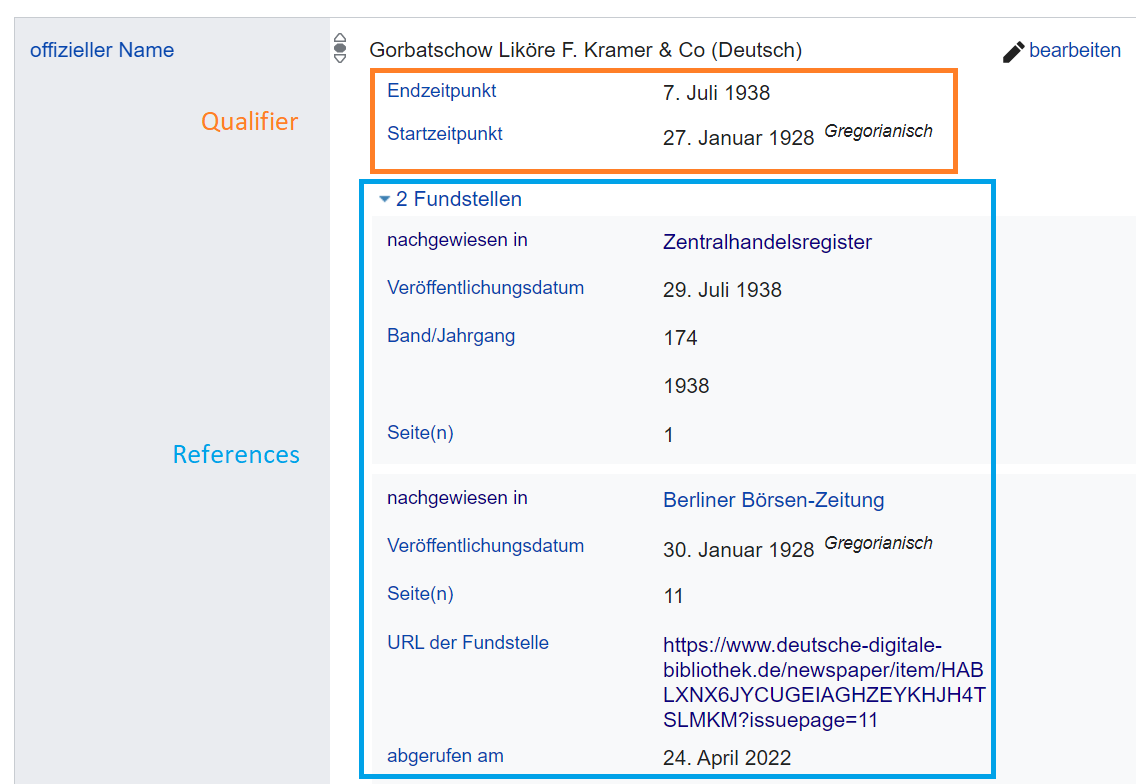
\includegraphics[width=\ScaleIfNeeded]{wikidata-reference}}
    \caption{Qualifikator und Fundstellen zu der Namensform ,,Gorbatschow Liköre F. Kramer \& Co'' des gleichnamigen Gewerbebetriebs.}
    \label{fig:x cubed graph}
\end{figure}

Wie in der Abbildung 4.9 an der zweiten Fundstelle außerdem zu sehen ist, kann ein permanenter Link zum gegenbenfalls im Web vorhandenen Quellendigitalisit hinterlegt werden. Falls dieses in einer Open Data-Lizenz veröffentlicht ist, bietet sich darüber hinaus an, es direkt in das Schwesternprojekt und in die öffentliche Bildersammlung \textit{Wikimedia Commons}\footnote{URL: \url{https://commons.wikimedia.org/wiki/Hauptseite} (letzter Zugriff am 28.05.2022).} hochzuladen. Dort gibt es bereits Bildmaterial zu Jüdischen Gewerbebetrieben vor allem in Zusammenhang mit der Reichspogromnacht 1938 sowie mit announcierten Besitzübernahmen, das bei zugehörigen Wikidata-Items direkt eingebunden werden kann (Abbildung 4.10).\footnote{Siehe Abfrage zu ,,Arisierung'' in Commons, URL: \url{https://commons.wikimedia.org/w/index.php?search=Arisierung&title=Special:MediaSearch&go=Go&type=image} (letzter Zugriff am 28.05.2022).}

\begin{figure}[h]
    \centering
    \frame{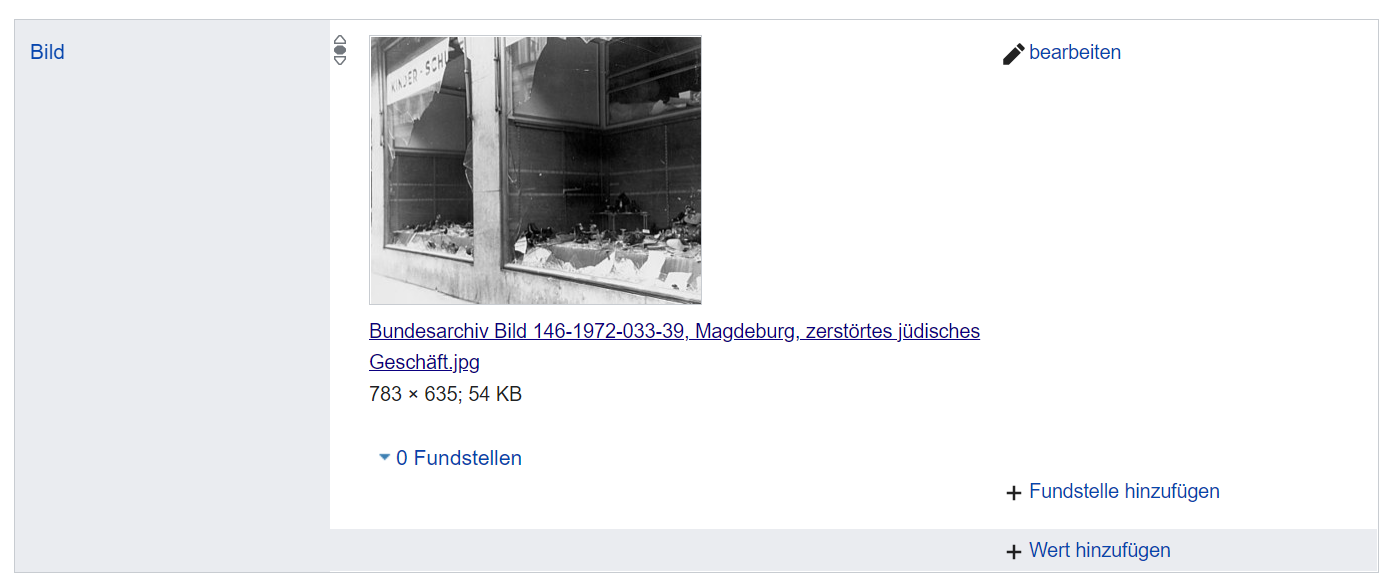
\includegraphics[width=\ScaleIfNeeded]{wikidata-commons}}
    \caption{Direkte Verknüpfung eines Fotodigitalisats aus Wikimedia Commons in Wikidata.}
    \label{fig:x cubed graph}
\end{figure}

Daraus ergibt sich erstmalig eine direkte Verknüpfung von Forschungsdaten und historischen Quellen, die eine bisher nie dagewesene Datenüberprüfung und -verifizierung ermöglicht und in der Konsequenz die Glaubwürdigkeit von Forschungsdaten im Forschungsfeld enorm steigern kann.\footnote{Auch in den Interviews wurde eine mögliche Verknüpfung als Funktionalität von offenem Forschungsdatenmanagement herausgehoben, vgl. Interview B3\_Transkript, Pos. 77.} 

Das Wikidata-Projekt kann daneben zur methodischen Führung sowie zur Entwicklung von Kriterien, welche Quellen sich als Belege für Jüdische Gewerbebetriebe eignen, genutzt und eine qualifzierte Quellensammlung im Forschungsfeld sukzessive aufgebaut werden.

\subsection{Erfassung von jüdischen Gewerbebtrieben}

Für die Erfassung der Daten zu jüdischen Gewerbebetriebe, so geht es aus den Interviews hervor, kamen herkömmliche Microsoft-Produkte wie Excel oder Access zum Einsatz.\footnote{Vgl. Interview B3\_Transkript, Pos. 11 und Interview B2\_Transkript, Pos. 27.} Es wurde folglich in erster Linie proprietäre, also kostenpflichtige, Software genutzt, die in der Regel nicht plattformunabhängig ist. Dies erschwert generell eine kollaborative Arbeit auf den Daten, denn die MS-Access-Anwendung zum Beispiel steht für Unix-basierte Betriebssysteme (Linux, Apple) gar nicht oder nur eingeschränkt zur Verfügung. Das heißt, dass grundlegende Open Source-Kritierien von diesen Produkten nicht erfüllt werden. 

Im Zusammenhang mit der Datenerfassung ist daher die wohl größte Herausforderung und aufwändigste Arbeit, ein User-Interface (UI) zu gestalten, das die bestmögliche User Experience und Usability (UX) bietet. Hier hält Wikidata nicht die perfekte Lösung bereit, aber zumindest Auswege aus möglichen anwendungsbedingten Einschränkungen und Zwängen, indem es nicht nur eine sondern mehrere Möglichkeiten der Erfassung von Daten gibt.\footnote{Siehe Wikidata:Datenspende, URL: \url{https://www.wikidata.org/wiki/Wikidata:Data\_donation/de\#Online-Tools\_=} (letzter Zugriff am 29.05.2022).} Von diesen werden drei nachfolgend vorgestellt, die sich an den bisherigen Kenntnisständen und Erfahrungen mit digitalen Werkzeugen im Forschungsfeld orientieren. 

Naheliegend ist die Eingabe der Daten im Linked Open Data Interface direkt auf der Website von Wikidata, wo per Mouseclick eines neues einzelnes Datenobjekt erstellt und erfasst werden kann (Abbildung 4.11). 

\begin{figure}[h]
    \centering
    \frame{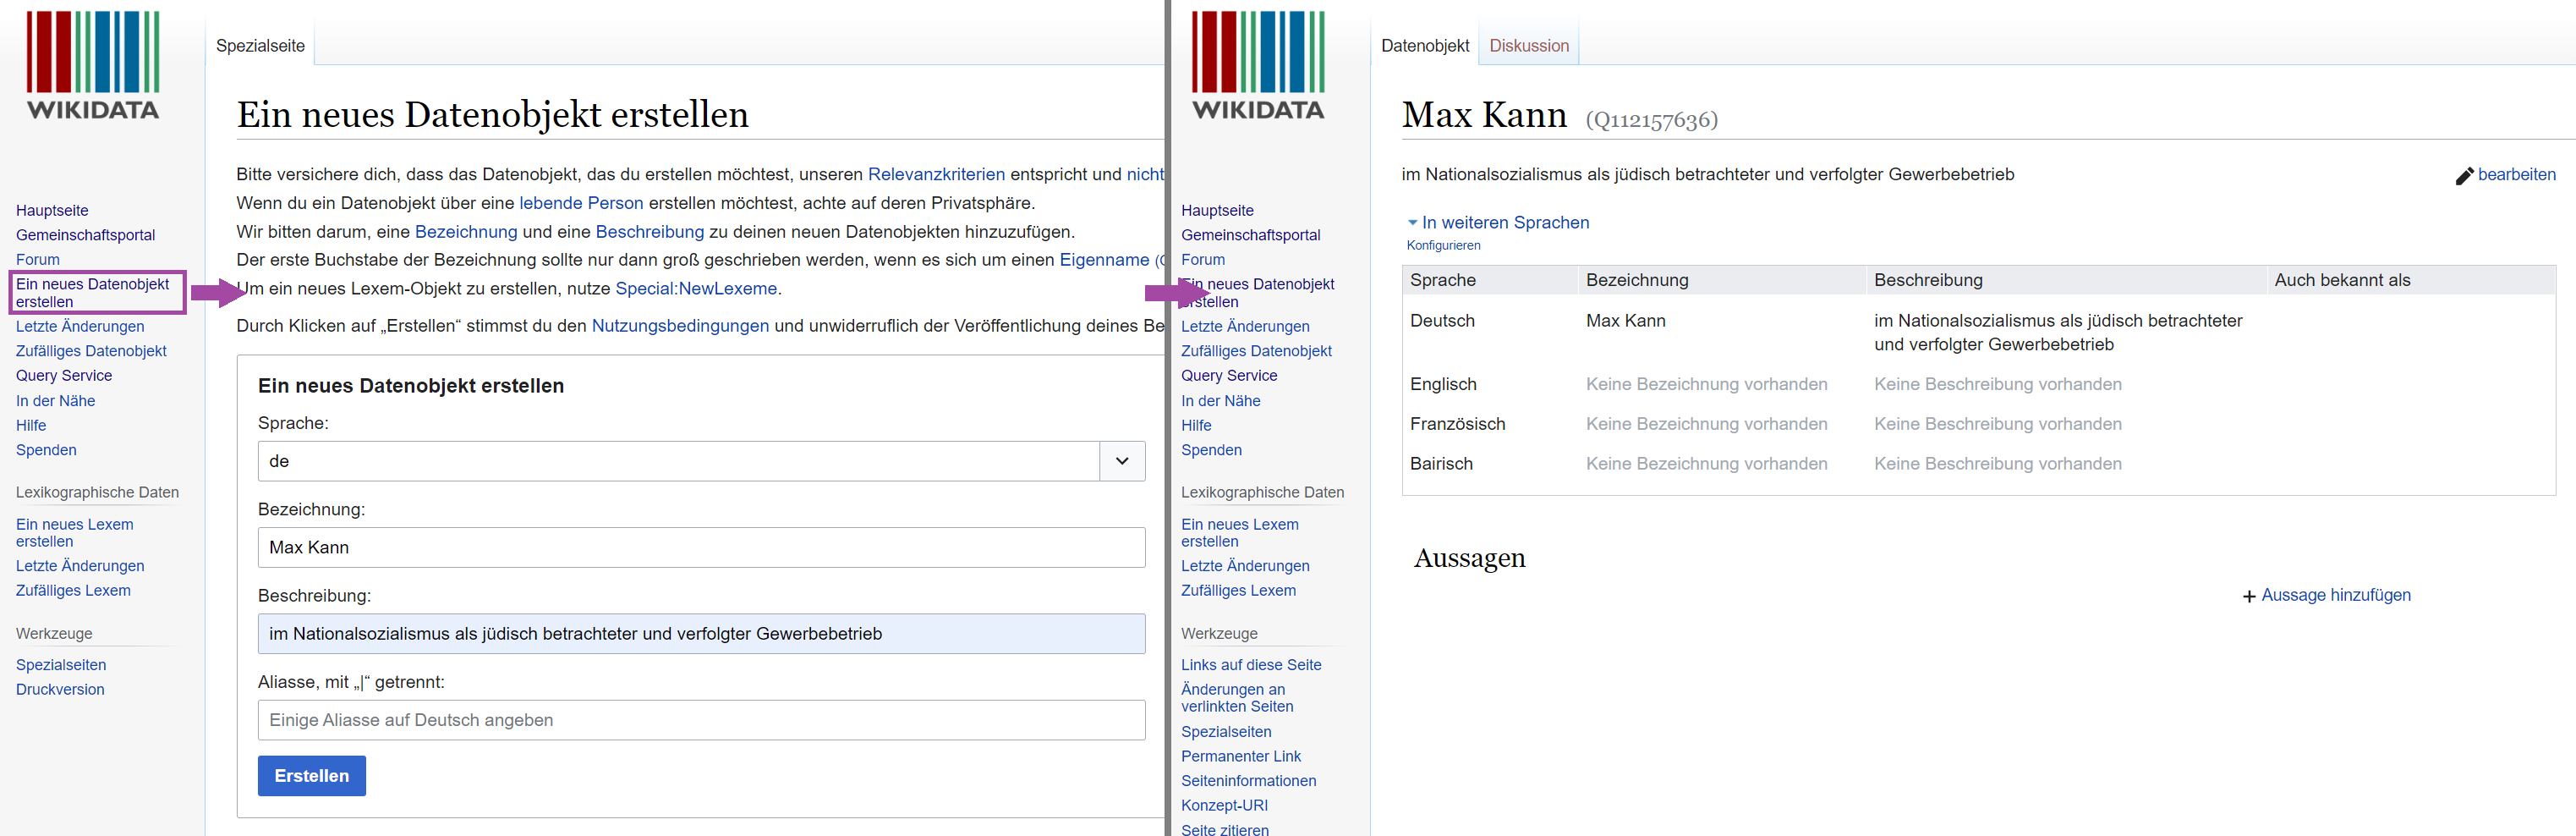
\includegraphics[width=\ScaleIfNeeded]{wikidata-linked-data-interface}}
    \caption{Links im Bild wird das Datenobjekt ,,Max Kann'' angelegt. Rechts ist das Item erstellt worden und es können weitere Daten erfasst werden.}
    \label{fig:x cubed graph}
\end{figure}

Diese Möglichkeit eignet sich besonders gut, wenn nur wenige Jüdische Gewerbebetriebe zur erfassen sind. Der Vorteil ist auch, dass ein Team gleichzeitig an der Eingabe von Daten arbeiten kann, was in den älteren Excel- oder Access-Desktopversionen nicht nicht möglich war.\footnote{Seit den Webversionen der Office-Sammlung von Microsoft kann allerdings auch in diesen kollaborativ gearbeitet werden. Siehe Microsoft Support (2022): Gleichzeitiges Bearbeiten von Excel-Arbeitsmappen mit der gemeinsamen Dokumenterstellung, URL: \url{https://support.microsoft.com/de-de/office/gleichzeitiges-bearbeiten-von-excel-arbeitsmappen-mit-der-gemeinsamen-dokumenterstellung-7152aa8b-b791-414c-a3bb-3024e46fb104}.} Mit steigender Zahl kann die Eingabe im Wikidata-Interface jedoch an Grenzen stoßen. Für Berlin, Frankfurt a.M. sowie Mannheim wurden jeweils Daten im 1.000er-Bereich erhoben.\footnote{In Berlin ca. 8.000, Frankfurt a.M. ca. 3.000 und Mannheim ca. 1.200.} Diese alle manuell und einzeln einzugeben, kostet vor allem Zeit, zumal diese bereits in Tabellenform vorliegen. In diesem Fall bietet sich die Stapel-Importfunktion (batch import) ,,QuickStatements'' an, bei der Daten, die als Tabstopp- oder Komma-separierte strukturierte Daten vorliegen, in Wikidata importiert werden.\footnote{URL: \url{https://quickstatements.toolforge.org/\#/batch} (letzer Zugriff am 29.05.2022).} Bevor der eigentliche Import jedoch erfolgen kann, bedarf es der Vorbereitung und Bereinigung der Daten. Zuerst müssen proprietären Formate in das offene CSV-Format transformiert werden, was zumindest für Excel-Dateien unproblematisch mit der Exportfunktion erfolgen kann (Abbildung 4.12).

\begin{figure}[h]
    \centering
    \frame{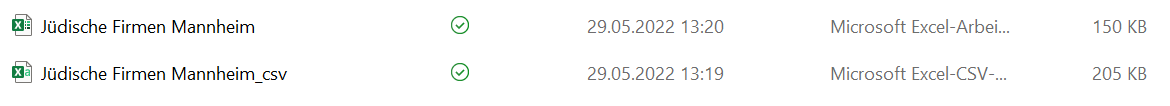
\includegraphics[width=\ScaleIfNeeded]{excel-csv}}
    \caption{Export der Excel-Tabelle mit Daten zu Jüdischen Gewerbebetrieben aus Mannheim in das CSV-Format.}
    \label{fig:x cubed graph}
\end{figure}

Bei den Access-Datenbanken ist diese Transformation aufwändiger, da hier das Problem hinzu kommt, dass es sich um veraltete Software-Versionen (2007) handelt, die sich mit neueren Versionen nicht mehr so einfach öffnen lassen. Für Berlin wurde kürzlich in einem eigenen Projekt diese Transformation durchgeführt.\footnote{Siehe Kapitel 1 Einleitung.} Im nächsten Schritt muss die ursprüngliche Datenstrukturierung in den transformierten CSV-Dateien an das Datenmodell des Wikidata-Projekts angepasst werden, wofür Wikidata ausführliche Hilfestellungen bereitgestellt hat.\footnote{Siehe Wikidata Help:QuickStatements, URL: \url{https://www.wikidata.org/wiki/Help:QuickStatements} (letzter Zugriff am 29.05.2022).} Dies wurde am Beispiel des Gewerbebetriebs \textit{Franz Mettner GmbH} aus Mannheim\footnote{URL (stable): url{https://www.wikidata.org/w/index.php?title=Q112163392\&oldid=1649916700}.} getestet (Abbildung 4.13).

\begin{figure}[h]
    \centering
    \frame{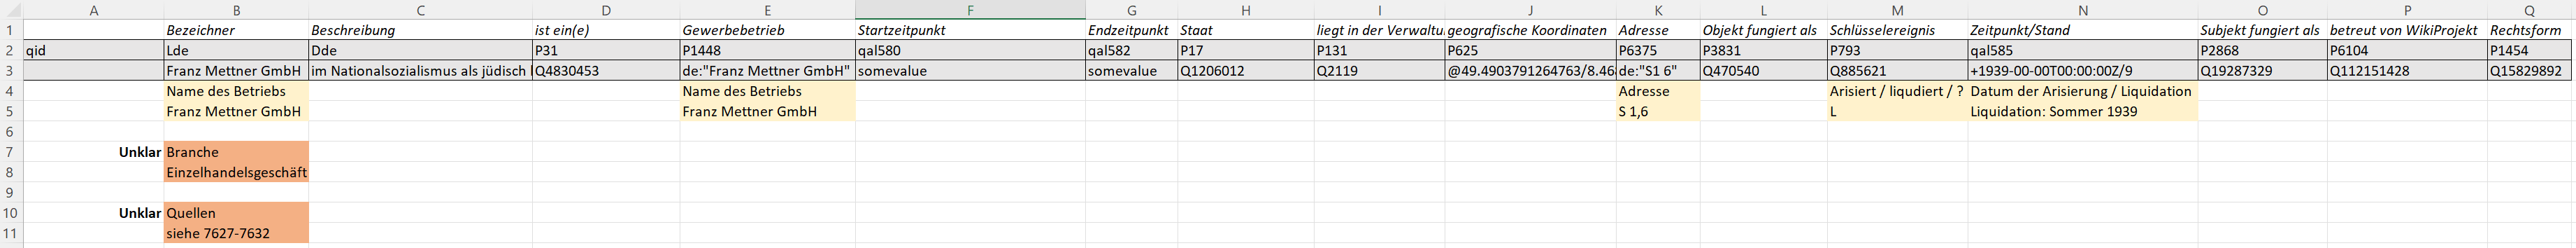
\includegraphics[width=\ScaleIfNeeded]{wikidata-bereinigung}}
    \caption{Datenvorbereitung und -bereinigung für den Import mit ,,QuickStatements''.}
    \label{fig:x cubed graph}
\end{figure}

Grau hinterlegt sind die Komma-separierten Werte, welche mit QuickStatements importiert wurden. Gelb und orange markiert sind die ursprünglichen Felder aus der Excel-Tabelle, welche dem Wikidata-Datenmodell zugeordnet werden konnten (gelb) und die Schwierigkeiten bereitet haben (orange). So scheint die Einordnung von ,,Einzelhandelsgeschäft'' unter Branche nicht treffend zu sein. Zudem sind die Quellenangaben ,,siehe 7627-7632'' nicht überprüfbar. Eventuell beziehen sich die Nummern auf ein projektinterne Verzeichnis, das aber nicht verfügbar ist. Das bedeutet, dass eine Verifizierung des Jüdischen Gewerbebetriebs allein mit der Excel-Tabelle für Externe nicht möglich ist. Hier müsste demnach vor dem Import die exakten Quellenangaben noch ergänzt werden. Der Import selbst in QuickStatements ist, sofern das Schema in der CSV-Datei korrekt ist, schnell erledigt (Abbildung 4.14).

\begin{figure}[h]
    \centering
    \frame{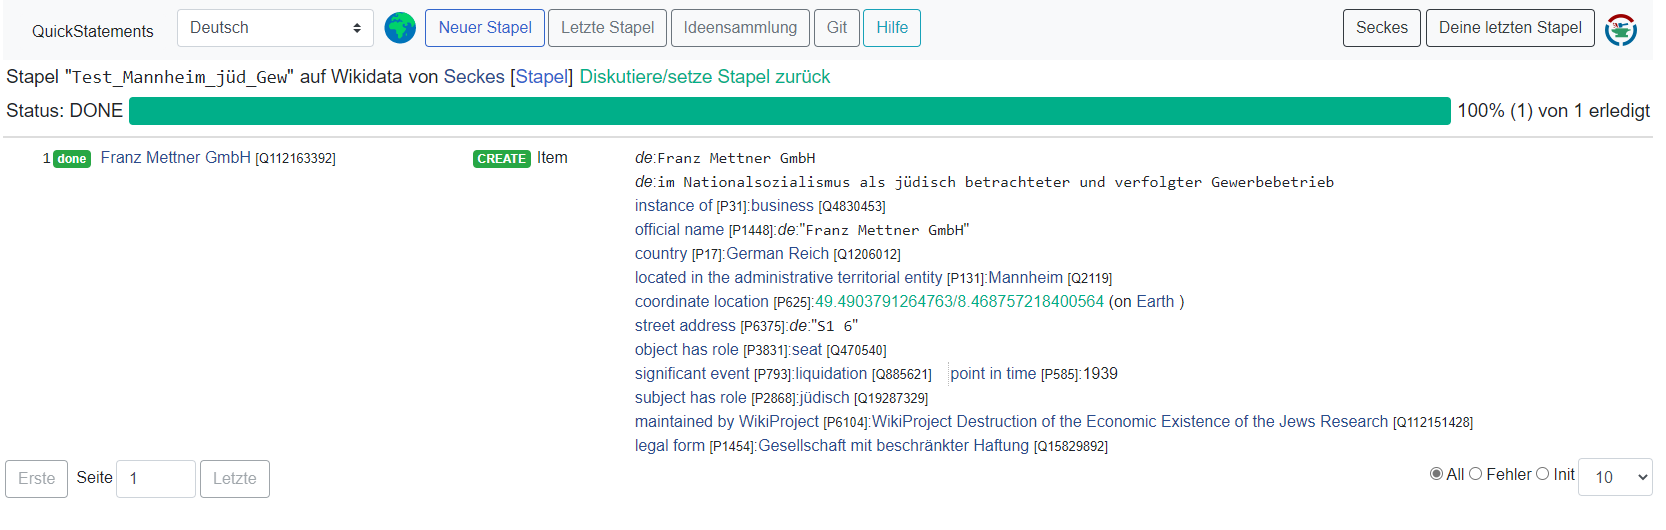
\includegraphics[width=\ScaleIfNeeded]{wikidata-quickstatements}}
    \caption{Erfolgreicher Import in QuickStatements.}
    \label{fig:x cubed graph}
\end{figure}

Während des Test-Imports zeigte sich, dass vor allem die Vorbereitung und Bereinigung der Daten für den Import zeitintensiv ist. Hier tauchen schließlich auch Probleme auf, die nicht immer vorhersehbar sind und für die eine Lösung gefunden werden muss. Dies betrifft insbesondere auch Freitextfelder, die von allen Studien verwendet und in denen unterschiedlichste Informationen festgehalten wurden. Diese lassen sich in Wikidata nicht importieren. Es ist nicht klar, welche Rolle diese Felder später bei der Auswertung spielten. Statistisch lässt sich damit jedenfalls nicht arbeiten. In einigen Fällen lassen sich die enthaltenen Daten auf den ersten Blick normalisieren, wenn zum Beispiel ,,1937 Emigration in die USA'' vermerkt ist. Schwieriger wird es bei Anmerkungen wie ,,1910 verlegte er sein Geschäft nach Mannheim (4-5 Arbeiter, die Ehefrau und der Sohn haben auch dort gearbeitet); 1937: wegen Hehlerei zu 1 Jahr, 4 Monaten und 2 Wochen Haft verurteilt Verbot zur Weiterführung des Geschäfts für 3 Jahre; nach USA emigiert''. Hieraus lassen sich drei Informationen extrahieren, die empirisch interessant sein können: Umzug, Anzahl Angestellte, Schicksal des Eigentümers. Wichtig wäre hier auch die Entscheidung, welche Daten nicht gebraucht und folglich kassiert werden.

\begin{figure}[h]
    \centering
    \frame{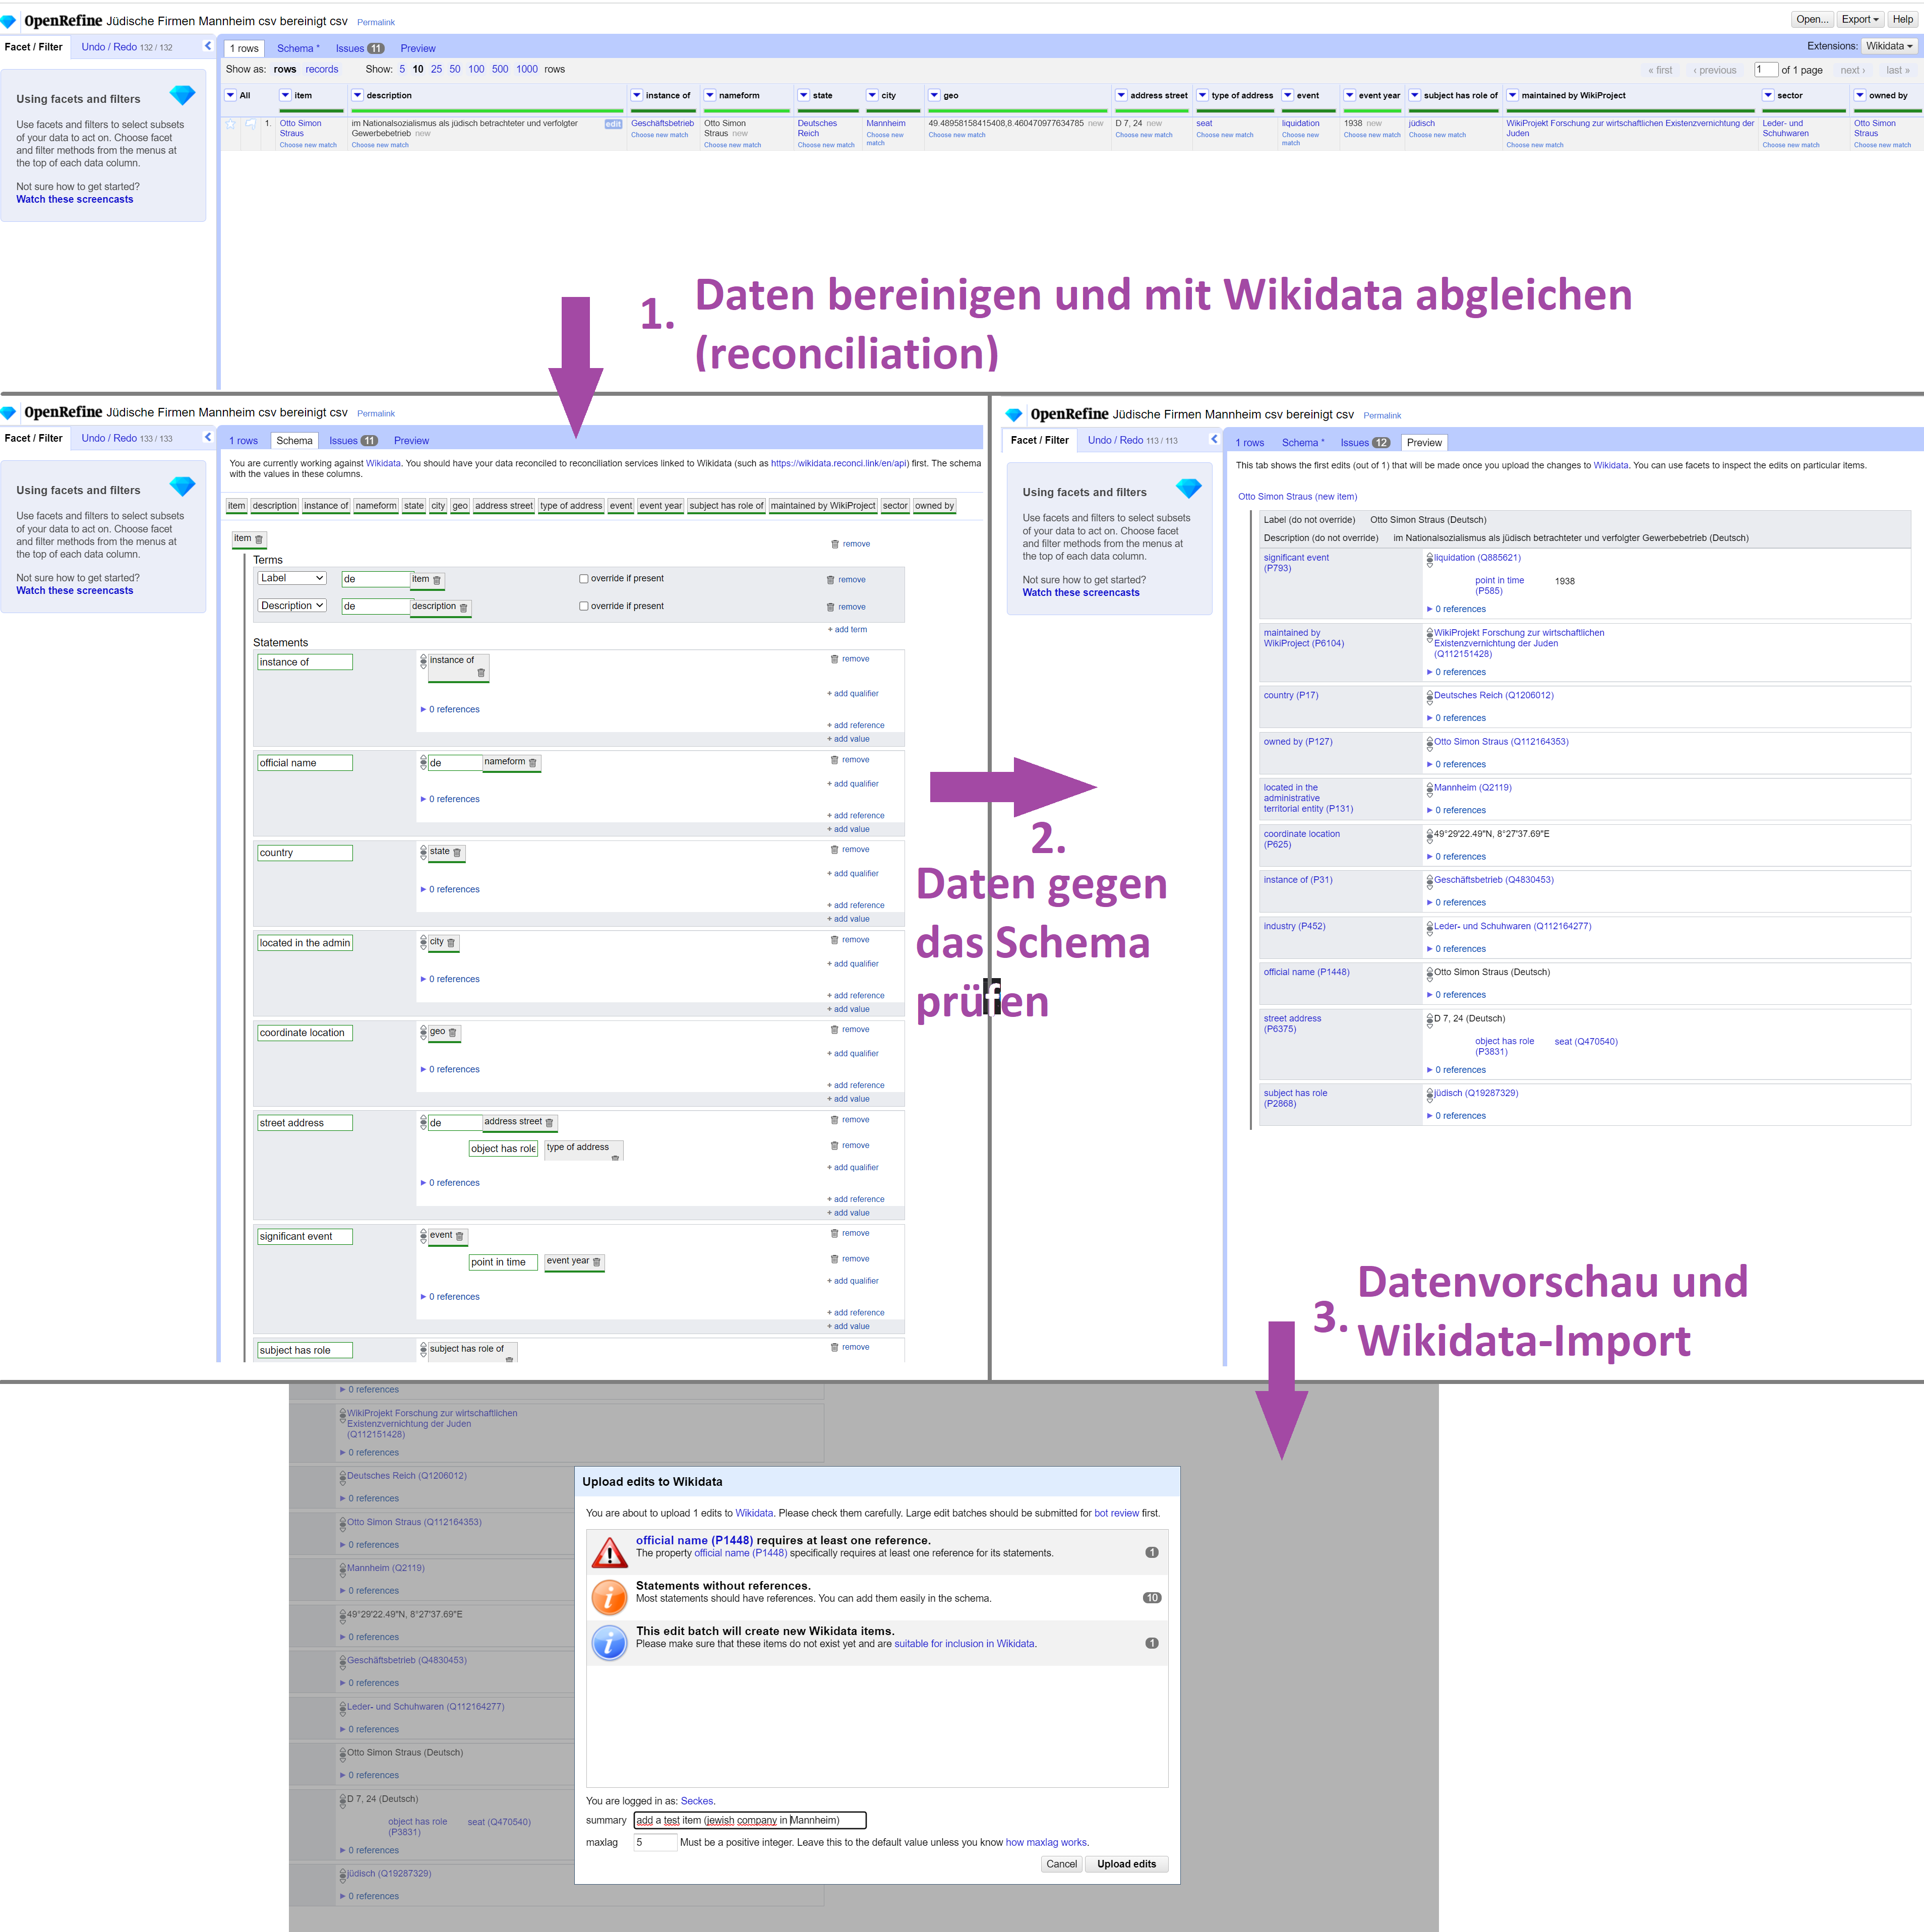
\includegraphics[width=\ScaleIfNeeded]{wikidata-pipeline}}
    \caption{Wikidata-Pipeline in Open Refine.}
    \label{fig:x cubed graph}
\end{figure}

Die dritte und letzte Option, die in dieser Arbeit vorgestellt wird, verdeutlicht, wie mit Wikidata Pipelines genutzt werden können, um optimale Workflows für die Datenerfassung in die Forschungsarbeit zu integrieren. Denn ein Nachteil von QuickStatements ist, dass die Daten aus den CSV-Dateien manuell in die Webanwendung kopiert werden müssen. Außerdem können die Daten in der Anwendung selbst nicht weiter überprüft werden. Hierfür ist das Open Source-Tool ,,Open Refine''\footnote{URL: \url{https://openrefine.org/} (letzter Zugriff am 29.05.2022).} besser geeignet. Die mächtige Anwendung, die auf die Bereinigung und Anreicherung von Massendaten spezialisiert ist, ermöglicht den Abgleich der Tabellendaten mit externen Wissensdatenbanken und darüber hinaus den Import direkt aus der Anwendung nach Wikidata (Abbildung 4.15).\footnote{Siehe Wikidata:Tools/OpenRefine, URL (stable:) \url{https://www.wikidata.org/w/index.php?title=Wikidata:Tools/OpenRefine\&oldid=1620901604}, Open Refine (2022): Overview of Wikibase support. Editing Wikidata with OpenRefine, URL: \url{https://docs.openrefine.org/manual/wikibase/overview\#editing-wikidata-with-openrefine} (letzter Zugriff am 29.05.2022).}

Die Kernfunktionen der Datenbereinigung werden hier nicht weiter erläutert, sondern auf die Wikidata-Upload-Pipeline fokussiert. In Abbildung 4.15 sind die Daten zum Jüdischen Gewerbebetrieb \textit{Otto Simon Straus} aus Manneheim\footnote{URL (stable): \url{https://www.wikidata.org/w/index.php?title=Q112166241\&oldid=1650023676}.} bereits von einer CSV-Datei in neu erstelltes Open Refine-Projekt hochgeladen worden. Die farbigen Balken unter jeder Titelspalte zeigen den Status des Abgleichs der Daten mit Wikidata an, welcher in Open Refine als ,,Reconciliation process'' bezeichnet wird. Dieser muss einmal für jede Titelspalte vorgenommen. Die dunkelgrünen Balken stehen für eindeutige Treffer (Abbildung 4.16 am Beispiel ,,Liquidation''), die hellgrünen für neue Werte und die grauen Balken für die noch abzugleichenden Daten. 

\begin{figure}[h]
    \centering
    \frame{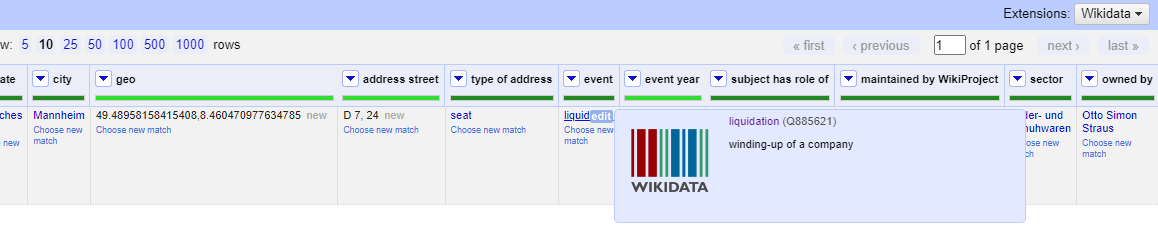
\includegraphics[width=\ScaleIfNeeded]{wikidata-reconciliation}}
    \caption{Eindeutiger Abgleich mit Wikidata in Open Refine.}
    \label{fig:x cubed graph}
\end{figure}

Im zweiten Schritt (in der Abbildung in der Mitte links) erfolgt die Prüfung der abgeglichenen Daten gegen ein Wikidata-Schema. Dies kann entweder direkt in Open Refine erstellt oder ein bestehendes als JSON-File importiert werden. Wenn für die Jüdischen Gewerbebetriebe demnach ein grundlegendes Datenmodell feststeht, kann dieses als JSON zum Beispiel im Wikidata-Projekt zur Verfügung gestellt und von jedem/ jeder in Open Refine wiederverwendet werden.\footnote{Zum Test wurde das in Open Refine erstellte Schema im Wikidata-Projekt hochgeladen, siehe URL: \url{https://www.wikidata.org/wiki/Wikidata:WikiProject\_Destruction\_of\_the\_Economic\_Existence\_of\_the\_Jews\_Research/Vernichtung\_der\_jüdischen\_Gewerbetätigkeit/Schema}.} Auf diese Weise sich eine Datenkontrolle bei der Dateneingabe im Forschungsfeld forcieren, was insgesamt zur Datenqualität beiträgt. Zum anderen ist es eine Arbeitserleichterung und bietet methodische Führung, wenn Schemata nachgenutzt und nicht für jedes Projekt von Grund auf neu erstellt werden müssen. Im dritten und letzten Schritt der Pipeline (Abbildung in der Mitte rechts sowie unten) lassen sich die Daten in einer Vorschau in Open Refine nochmals überprüfen, bevor sie in Wikidata importiert werden.\footnote{Permalink zum lokalen Projekt (localhost) URL: \url{http://127.0.0.1:3333/project?project=2437124036317\&ui=\%7B\%22facets\%22\%3A\%5B\%5D\%7D}.} Der Nachteil von Open Refine ist, dass die Möglichkeiten der kollaborativen Arbeit an einem Projekt noch begrenzt sind. Bisher können diese nur manuell zusammengeführt werden.\footnote{Siehe Consortium Historicum (2018): Ergänzen eines OpenRefine-Projekts mit einem anderen, Blogbeitrag auf histHub am 26.02.2018, URL: \url{https://histhub.ch/ergaenzen-eines-openrefine-projekts-mit-einem-anderen/} (letzter Zugriff am 30.05.2022).} 

Auch wenn die diversen Möglichkeiten des Datenimports in Wikidata zunächst überfordern können\footnote{Neben den drei vorgestellten Tools gibt es auch noch die REST-Api von Wikimedia sowie die Möglichkeit der Verwendung von Bots. Auch Wikimedia Cloud Services-Projekte mit weiteren Werkzeugen befinden im Aufbau, URL: \url{https://wikitech.wikimedia.org/wiki/Help:Cloud_Services_introduction} (letzter Zugriff am 30.05.2022).}, ist der Vorteil insgesamt, dass durch diese Vielseitigkeit die Datenerfassung an jeweilige Use Cases und an Nutzungsgewohnheiten optimal angepasst werden kann. Auch vor dem Hintergrund, dass immer mehr historische Quellen digitalisiert vorliegen, was einen automatisierten Import ermöglicht, werden diese vielfältigen Services des Datenimports zunehmend notwendig.\footnote{Das NFDI-Konsortium nfdi4Culture organisiert Ende Juni einen Workshop, der sich explizit mit der Wikibase-Upload-Pipeline in Open Refine beschäftigt, siehe URL: \url{https://nfdi4culture.de/news-events/events/jcdl-workshop-open-refine-to-wikibase-a-new-data-upload-pipeline.html} (letzter Zugriff am 29.05.2022).} Die Kehrseite dieser Werkzeugvielfalt ist, dass sich die Einarbeitungszeit mit jedem neuen Tool, das genutzt wird, insgesamt verlängert.

\subsection{Verknüpfung von Sample und Fallbeispielen}

Mehrmals wurde in den Interviews betont, dass die rein quantitative Arbeit im Forschungsfeld lediglich einen Teil der Forschung zur Vernichtung der jüdischen Gewerbetätigkeit ausmacht.\footnote{Vgl. Interviews B2\_Transkript, Pos. 53, 63 und B3\_Transkript, Pos. 83.} Den anderen Teil bilden Fallbeispiele, die vor allem zeigen, dass der Prozess der Verfolgung und Vernichtung von zahlreichen Einzelfaktoren abhing und auf der individuellen Ebene daher sehr unterschiedlich verlaufen konnte. Neben diesen Einzelfallstudien gibt es außerdem die Gedenkbücher in analoger oder digitaler Form, die einen stark dokumentarischen Charakter aufweisen, der sich vorwiegend in einem deskriptiven Zusammentragen von verteilten Informationen zu jüdischen Gewerbebetrieben und jüdischen Unternehmern zeigt.\footnote{Nietzel hebt hier die akribisch recherchierte Textsammlung zu jüdischen Unternehmen in München des Archivars und Historikers Wolfgang Selig aus dem Jahr 2004 hervor, vgl. Nietzel 2009, S. 583.} Hierunter zählen auch jene Veröffentlichungen, die nicht primär auf Daten zu jüdischen Gewerbebetrieben fokussiert sind, sondern wo diese von anreichernder Bedeutung sind.\footnote{Hier vor allem die zahlreichen Gedenkbücher zu jüdischen Personen, die mittlerweile online zugänglich sind und wo sich Daten zu jüdischen Gewerbebetrieben in den Biogrammen der Personen ,,verstecken''. Siehe zum Beispiel ,,Biografisches Gedenkbuch der Münchner Juden 1933–1945'' der Stadt München, URL: \url{https://gedenkbuch.muenchen.de/} (letzter Zugriff am 12.05.2022). Bei der Biografie von Max Hofman ist unter ,,Weitere Informationen'' vermerkt: ,,Max Hofmann war Inhaber der Fa. Max Hofmann, einem Großhandel und Versand von Manufaktur- und Textilwaren, in der Paul-Heyse-Straße 28/I. Das Gewerbe wurde am 17.10.1938 für den 15.10.1938 abgemeldet.'', URL (stable): \url{https://gedenkbuch.muenchen.de/index.php?id=gedenkbuch_link&gid=5722}.} Diese Datenvielfalt im Forschungsfeld lässt sich wie folgt zusammenfassen: 

\begin{enumerate}
    \item Es gibt \textbf{quantitative (Massen-)Daten}, die strukturiert, entweder als Rohdaten oder in aggregierter Form, vorliegen. Sie besitzen eine statistische Aussagekraft.
    \item Es gibt \textbf{qualitative Daten}, die in der Regel textuell und damit unstrukturiert oder semistruktiert vorliegen.
\end{enumerate}

Bereits Nietzel beklagte in seinem Forschungsbericht aus dem Jahr 2009, dass die qualitativen Daten insbesondere aus der Gedenk- und Erinnerungskultur für eine wissenschaftliche analytische Auswertung bislang zu unsystematisch sind.\footnote{Nietzel 2009, S. 583.} Umgekehrt fehlt den statistischen Massendaten ihres Umfang wegens oft die entsprechende Datentiefe und die Einzelschicksale und -geschichten hinter der Statistik bleiben unsichtbar.\footnote{Allein für Berlin hat die Stichprobe einen Umfang von ca. 8.000 jüdischen Gewerbebetrieben. Auch für Frankfurt am Main sind es in der Stichprobe über 2.500 jüdische Gewerbebtriebe. Vgl. Kreutzmüller 2012, URL: \url{https://www2.hu-berlin.de/djgb/www/find} (letzter Zugriff am 07.05.2022) und Nietzel 2012, S. 15.} Das macht diese Daten vor allem außerhalb der wissenschaftlichen Forschung weniger greif- und nutzbar. 

\begin{figure}[h]
    \centering
    \frame{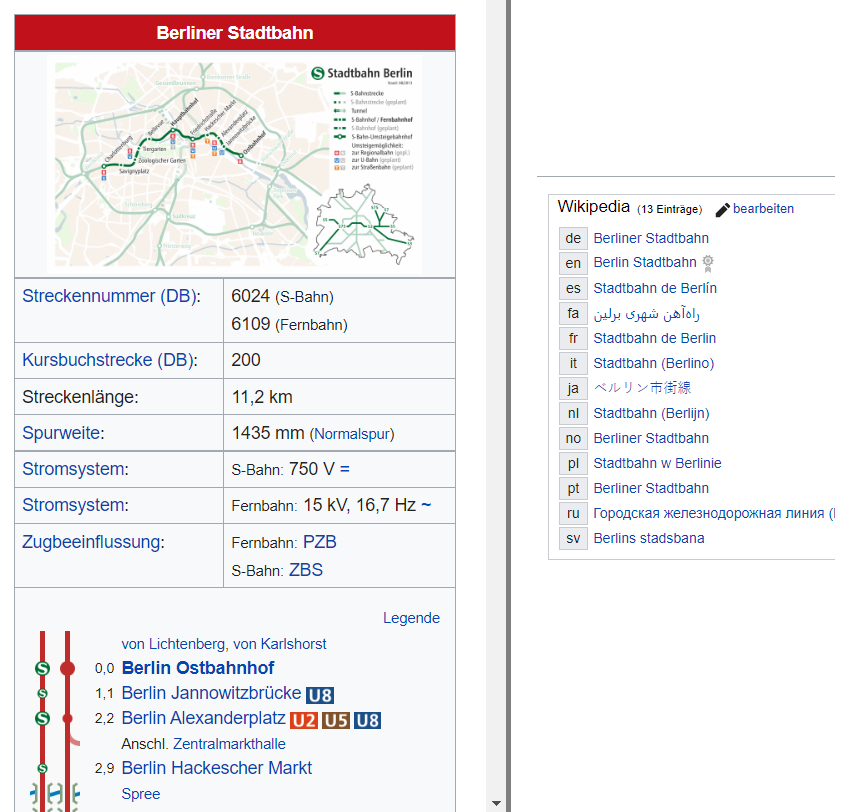
\includegraphics[scale=0.4]{wikidata-wikipedia}}
    \caption{In Wikipedia werden Wikidata-Daten üblicherweise für kompakte Infoboxen genutzt, hier am Beispiel des Artikels zur Berliner Stadtbahn (links). In Wikidata wiederum lässt sich dem Item Berliner Stadtbahn (Q694223) der Wikipedia-Artikel aller Sprachversionen eindeutig zuordnen (rechts).}
    \label{fig:x cubed graph}
\end{figure}

Festzuhalten ist, dass es bisher im Forschungsfeld noch nicht gelungen ist, quantitative und qualitative Forschungsdaten zu verknüpfen. Es ist aber eben diese Verknüpfung der verteilten Datenvielfalt, die im Wiki*versum gängige Praxis ist. Dies wurde bereits anhand der Quellendigitalisite in ,,Wikimedia Commons'' und deren Integration in Wikidata deutlich.\footnote{Vgl. Kapitel 4.3.2 Quellennachweise.} Gleiches lässt sich auch auf der Textebene mit der Enzyklopädie \textit{Wikipedia} realisieren. Analog zu Wikidata-Projekten gibt es in der Wikipedia Themenportale, die sich auf das Schreiben von Wikipedia-Artikeln zu einem bestimmten Thema spezialisiert haben.\footnote{Portal:Wikipedia nach Themen, URL: \url{https://de.wikipedia.org/wiki/Portal:Wikipedia_nach_Themen} (letzter Zugriff am 30.05.2022).} Unter den Rubriken ,,Geschichte'' oder ,,Wissenschaft'' gibt es thematisch dem Forschungsfeld nahestehende Portale wie das ,,Portal:Geschichte des 20. Jahrhunderts''\footnote{URL (stable): \url{https://de.wikipedia.org/w/index.php?title=Portal:Geschichte\_des\_20.\_Jahrhunderts\&oldid=216577544}.} oder ,,Portal:Geschichte''\footnote{URL (stable): \url{https://de.wikipedia.org/w/index.php?title=Portal:Geschichte\&oldid=215435556}.} Es kann jedoch auch ein neues Themenportal angelegt werden. Im Wikipedia-Artikel können die strukturierten Daten aus Wikidata üblicherweise in einer kompakten Infobox hinzugefügt werden, während dem zugörigen Wikidata-Item der Wikipedia-Artikel verknüpft wird (Abbildung 4.16).\footnote{Siehe zur Umsetzung der Verknüpfungen die Dokumentationsseite ,,Wikidata:Wie man Daten in Wikimedia-Projekten nutzt'', URL: \url{https://www.wikidata.org/wiki/Wikidata:How_to_use_data_on_Wikimedia_projects/de} (letzter Zugriff am 30.05.2022).}

Im Rahmen dieser Arbeit liegt der Schwerpunkt auf den strukturierten (Massen)Daten und damit auf Wikidata. Somit bleiben die Möglichkeiten der Verbindung zu Wikipedia hier nur angedeutet. Sie zeigen aber bereits die Potentiale, die sich über Wikidata hinaus im Wiki*versum für das Forschungsfeld ergeben. So können kollaborativ ,,Geschichten'' zu Jüdischen Gewerbebetrieben gesammelt und diese in Wikipedia-Artikeln veröffentlicht werden, die für alle zugänglich und nachnutzbar sind. Gleichzeitig können aus den Artikeln Daten extrahiert, strukturiert in Wikidata erfasst und dort ebenfalls nachgenutzt werden.

\section{Analyse}

\begin{quote}
    ,,Ich hatte da auch bestimmte Ideen, dass man auch so auf städtischen Karten mal einzeichnen könnte, wo die ganzen Unternehmen lagen, wo die sich gehäuft haben. Das fände ich super spannend, aber das ist super viel Arbeit und ich kann das selber gar nicht machen.''\footnote{Interview B2\_Transkript, Pos. 67.}
\end{quote}

Für die finale Datenauswertung kam im Forschungsfeld einfache deskriptive Statistik zur Anwendung. Es ging also zuvorderst darum, die Forschungsdaten zu Jüdischen Gewerbebetrieben den Forschungsfragen entsprechend zu ordnen und übersichtlich darzustellen. Dies geschah überwiegend in Tabellenform. Nur im Fall von Berlin wurden die Daten auch mit statistischen Schaubildern wie Karten, Balken- und Liniendiagrammen graphisch präsentiert. In dieser aggegrierten Form sind sie in den Publikationen der Lokalstudien zugänglich. Mit welchen Tools exakt die Datenauswertung der einzelnen Studien realisiert wurde, ist nicht bekannt. Aus den Lokalstudien lässt sich aber schließen, dass für die Datenanalyse keine komplexen Berechnungen sondern in der Regel einfache Datenabfragen (Queries) ausreichen. 

Wikidata bietet neben der Speicherung von Daten auch deren Abfrage mit dem eigenen ,,Wikidata Query Service'' an.\footnote{Wikidata Query Service, URL: \url{https://query.wikidata.org/} (letzter Zugriff am 30.05.2022).} Dies erfolgt mit der globalen Linked Open Data- und RDF-Abfragesprache \textit{SPARQL} (SPARQL Protocol And RDF Query Language), welche seit 2013 vom ,,World Wide Web Consortium'' (W3C) als offizielle Spezifikation veröffentlicht und folglich zum Standard erklärt wurde.\footnote{Vgl. W3C (2013): SPARQL 1.1 Overview. W3C Recommendation 21 March 2013, URL: \url{http://www.w3.org/TR/2013/REC-sparql11-overview-20130321/} (letzter Zugriff am 30.05.2022).} Ein grundlegender Unterschied zur konventionellen SQL-Datenabfragesprache (Structured Query Language) in relationalen Datenbanken besteht darin, dass mit SPARQL unter der Verwendung von ,,Namespaces'' über Datenquellen hinweg Daten abgefragt werden können, während mit SQL nur auf der eigenen Datenbasis gearbeitet werden kann. Gerade hier liegt eine der Stärken von Linked Open Data und des Semantic Webs, nämlich verteilte Informationen die im RDF-Format gespeichert sind, zu beschaffen und zu verarbeiten. 

In der Benutzeroberfläche des Query Service werden die SPARQL-Abfragen geschrieben und können dort direkt ausgeführt werden. Standardmäßig wird das Ergebnis in Tabellenform ausgegeben. Doch hat Wikidata zahlreiche weitere Tools vor allem für die Darstellung und Visualisierung von Daten im Angebot.\footnote{Eine Übersicht über die Werkzeuge für Wikidata siehe Wikidata:Tools, URL: \url{https://www.wikidata.org/wiki/Wikidata:Tools}. Siehe auch Wikidata:SPARQL query service/Wikidata Query Help/Result Views/de, URL: \url{https://www.wikidata.org/wiki/Wikidata:SPARQL_query_service/Wikidata_Query_Help/Result_Views/de} (alle letzter Zugriff am 30.05.2022).} Neben der reinen Präsentation von Daten können sie auch als Methode für eine (visuelle) Datenexploration aufgegriffen werden, die neue Perspektiven auf die Daten eröffnet und mit der schrittweise ein detailliertes Verständnis von den Daten entwickelt werden kann.\footnote{Vgl. H. Degen: Graphische Datenexploration, in: C. Wolf, H. Best (Hrsg.), Handbuch der sozialwissenschaftlichen Datenanalyse, Wiesbaden 2010, S. 91ff., doi:10.1007/978-3-531-92038-2\_5.} 

In den nachfolgenden Kapiteln soll es vordergründig darum gehen, die Möglichkeiten der graphische Datenexploration in Wikidata für das Forschungsfeld nutzbar zu machen, da es hier auch - wie das einleitende Zitat zeigt - Bedarf gibt. Aber auch sich neu ergebende Forschungsfragen sollen antizipiert sowie Datenqualität allgemein beurteilt werden. Dabei werden im Rahmen dieser Arbeit nicht alle Forschungsfragen im Sinne einer Replikationsstudie bearbeitet, sondern exemplarisch vor allem die Möglichkeiten einer Datenanalyse mit Wikidata gezeigt. Zu diesem Zweck wurden in Wikidata drei Beispieldatensätze angelegt, die zufällig aus den vorliegenden Forschungsdaten zu Berlin, Mannheim und Krefeld ausgewählt wurden:

\begin{itemize}
    \item Gorbatschow Liköre F. Kramer \& Co (Q112127138), Berlin\footnote{URL: \url{https://www.wikidata.org/w/index.php?title=Q112127138\&oldid=1651194448}.}
    \item Otto Simon Straus (Q112166241), Mannheim\footnote{URL: \url{https://www.wikidata.org/w/index.php?title=Q112166241\&oldid=1651188294}.}
    \item Franz Mettner GmbH (Q112163392), Mannheim\footnote{URL: \url{https://www.wikidata.org/w/index.php?title=Q112163392\&oldid=1651187976}.}
\end{itemize}

\subsection{Gewerbestruktur}

\paragraph{Branchen} Die Verteilung der Jüdischen Gewerbebetriebe wurde von allen Lokalstudien untersucht, denn damit konnten zum einen Aussagen zu deren Anteil und Bedeutung für die lokale Wirtschaft gemacht werden. Zum anderen wurde herausgearbeitet, welche Branchen die Verfolgung und Vernichtung zuerst und besonders stark trafen beziehungsweise ob es Branchen gab, die relativ verschont blieben. Mit SPARQL kann dazu eine einfache Abfrage erstellt werden. Voraussetzung dafür ist, dass einheitliche Branchenname verwendet werden, was aber für die Lokalstudien insgesamt nicht zutrifft. Für die Beispieldatensätze wurden die Branchen unter Nachnutzung der ,,Branchensystematikstelle des Pressearchiv 20. Jahrhundert'' vereinheitlicht.\footnote{Siehe Wikidata:WikiProject 20th Century Press Archives, URL: \url{https://www.wikidata.org/w/index.php?title=Wikidata:WikiProject\_20th\_Century\_Press\_Archives\&oldid=1562096427}.} Eine Abfrage über deren vorhandene Datenobjekte zeigt jedoch, dass nicht alle Branchen, welche für die Jüdischen Gewerbebetriebe benötigt werden, vorhanden sind (Abbildung 4.18).\footnote{Short-URL der Abfrage: \url{https://w.wiki/5DpB}.} 

\begin{figure}[h]
    \centering
    \frame{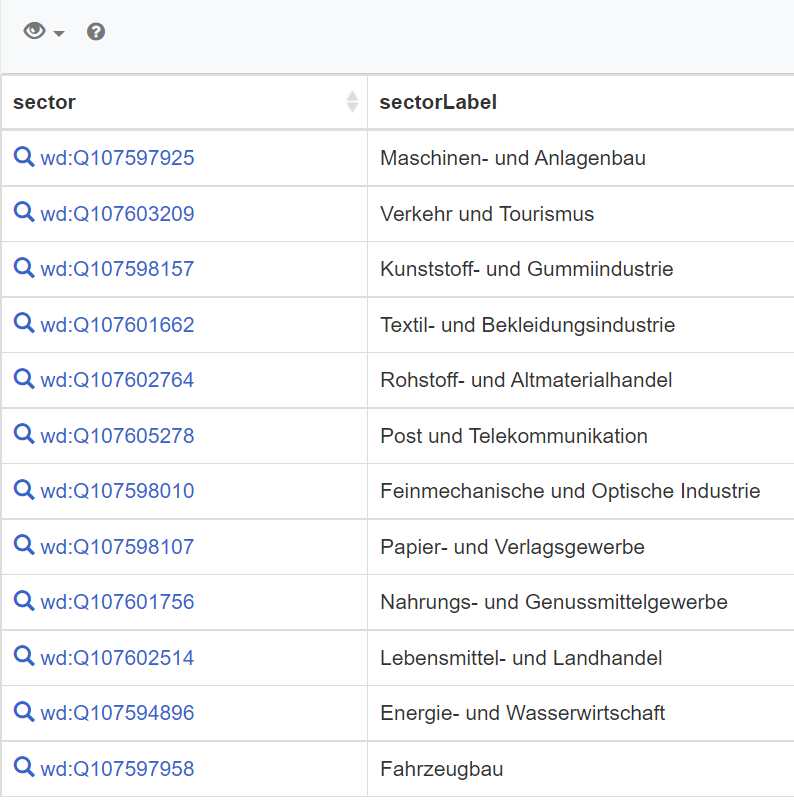
\includegraphics[scale=0.5]{wikidata-sectors-pressearchiv}}
    \caption{Branchensystematik des Pressearchiv 20. Jahrhundert.}
    \label{fig:x cubed graph}
\end{figure}

\begin{figure}[h]
    \centering
    \frame{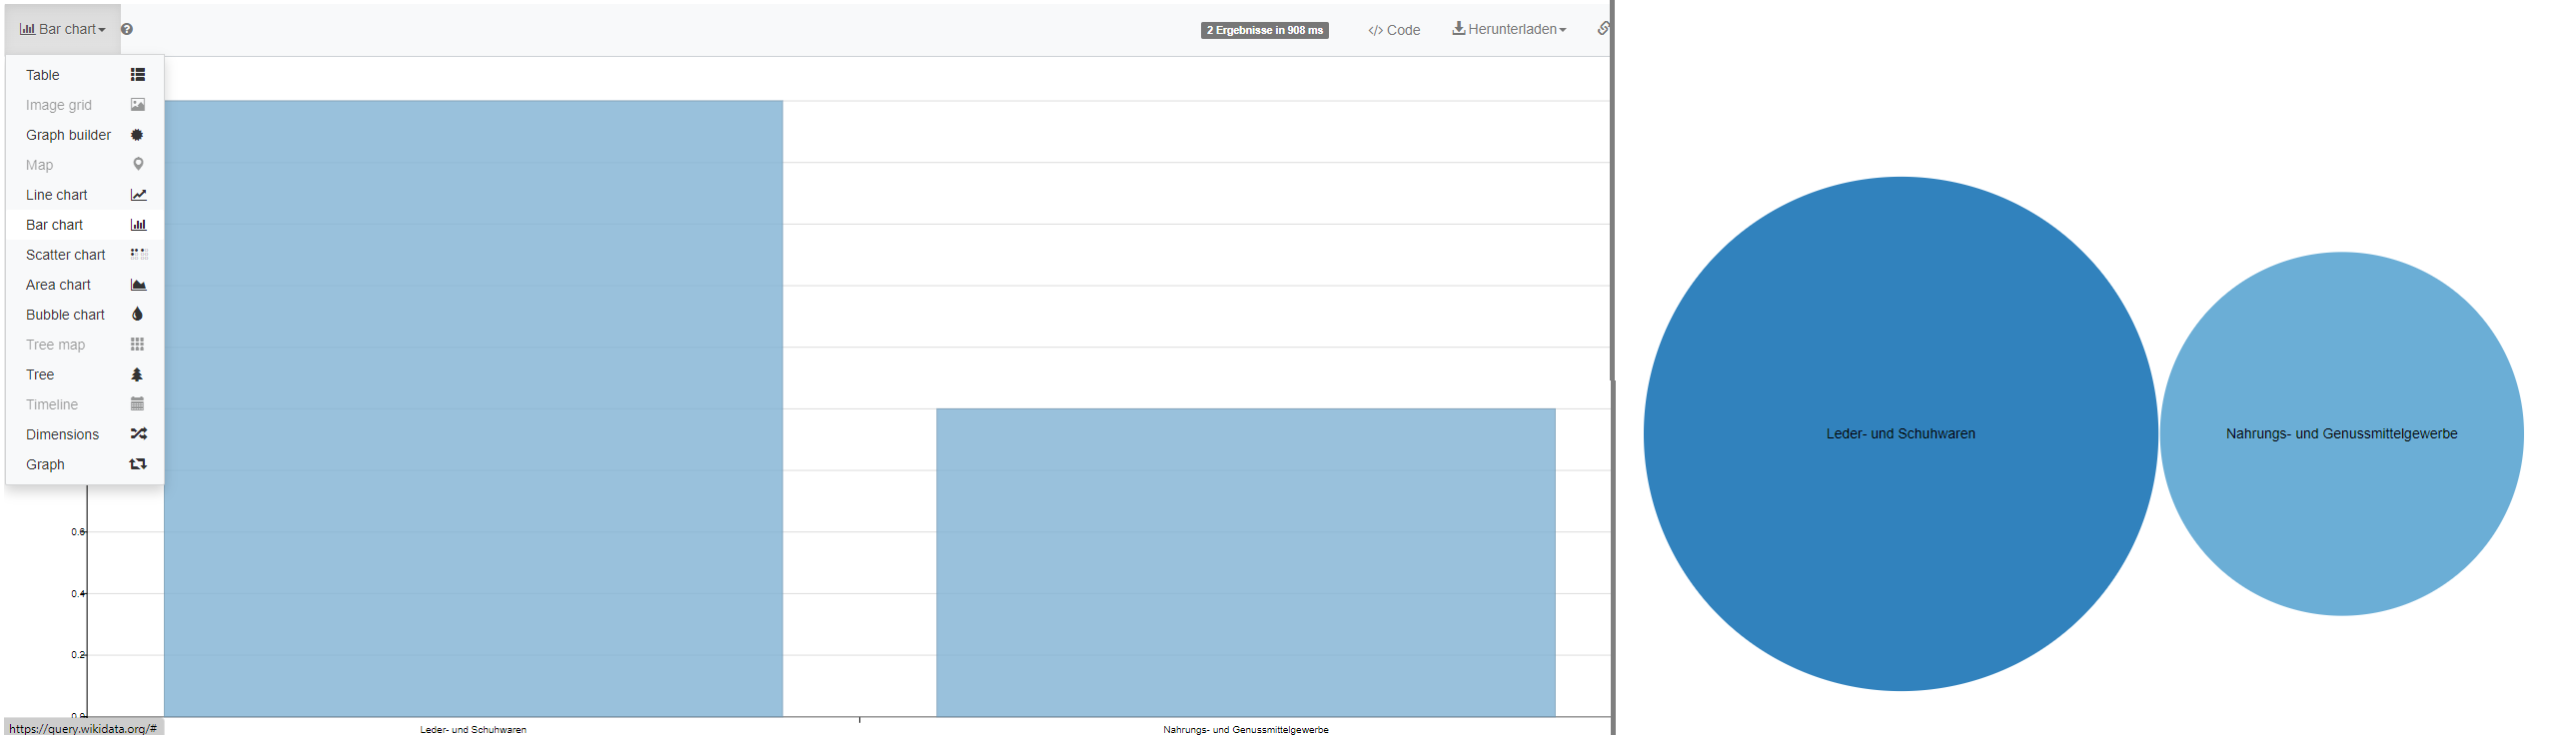
\includegraphics[width=\ScaleIfNeeded]{wikidata-bar-bubble}}
    \caption{Visualisierung der Ergebnisse zur Branchenverteilung mit Säulendiagramm (links) und Bubble Chart (rechts).}
    \label{fig:x cubed graph}
\end{figure}

In diesem Fall kann eine ergänzende Systematik entwickelt und in Wikidata hinzugefügt werden. Hierfür wurde im Wikidata-Projekt ein erster Vorschlag für das Forschungsfeld auf Basis der Branchenliste aus der Berliner Studie unterbreitet.\footnote{URL: \url{https://www.wikidata.org/w/index.php?title=Wikidata_talk:WikiProject\_Destruction\_of\_the\_Economic\_Existence\_of\_the\_Jews\_Research/Vernichtung\_der\_jüdischen_Gewerbetätigkeit\&oldid=1651252043}.} In Wikidata können die Abfrageergebnisse direkt im Query Service als Diagramme wie Bar Chart oder Bubble Chart visualisiert (Abbildung 4.19) oder aber das externe ,,Wikidata Visualization''-Tool verwendet werden, welches noch mehr Auswahl bei der Darstellung hat.\footnote{Wikidata Visualization, URL: \url{https://dataviz.toolforge.org/} (letzter Zugriff am 31.05.2022).} Gibt es eine gemeinsame Branchensystematik für das Forschungsfeld, ließe sich damit erstmals insgesamt und im Städtevergleich die Branchenstruktur untersuchen, was sich zum Beispiel durch ein Multi-Säulendiagramm gut explorieren ließe.\footnote{Siehe hierzu auch die Wikipedia-Dokumentation ,,Graph:Stacked'', URL: \url{https://de.wikipedia.org/w/index.php?title=Vorlage:Graph:Stacked\&oldid=198988739}.}

\paragraph{Verteilung im Stadtraum}

In den Interviews wurde explizit auch die Möglichkeit der topografischen Untersuchung von Jüdischen Gewerbetrieben erwähnt, um deren Verteilung im Stadtraum und etwaige Ballungszentren zu untersuchen. Hierfür braucht es allerdings die Koordinatenpunkte der Gewerbebetriebe, die dessen topografische Lage eindeutig bestimmen. Diese Daten werden als Geodaten bezeichnet und stellen einen eigenen Datentyp dar.\footnote{Vgl. Wikidata-Property geographische Koordinaten (P625), URL: \url{https://www.wikidata.org/wiki/Property:P625}.} Ohne selbst dafür eine Anwendung aufwändig programmieren zu müssen, wird in Wikidata einerseits automatisch der Standort eines Datenobjekts direkt in einem Kartenausschnitt ausgegeben werden, wenn geographische Koordinatenpunkte als Property hinterlegt sind, und können andererseits Standorte mit SPARQL abgefragt und auf einer Karte visualisiert werden. Die größte Hürde in Bezug auf das Forschungsfeld stellt daher nicht die Kartenvisualisierung an sich dar. Es sind die fehlenden geographischen Daten, die bisher von keiner Lokalstudien erfasst wurden und die demzufolge nachträglich ergänzt werden müssten. Erst mit diesen ließe sich eine Verteilung von Jüdischen Gewerbebetrieben im Stadtraum sowie erstmals auch deutschlandweit visuell untersuchen (Abbildung 4.20).\footnote{Short-URL zur Abfrage: \url{https://w.wiki/5Dsz}.}

\begin{figure}[h]
    \centering
    \frame{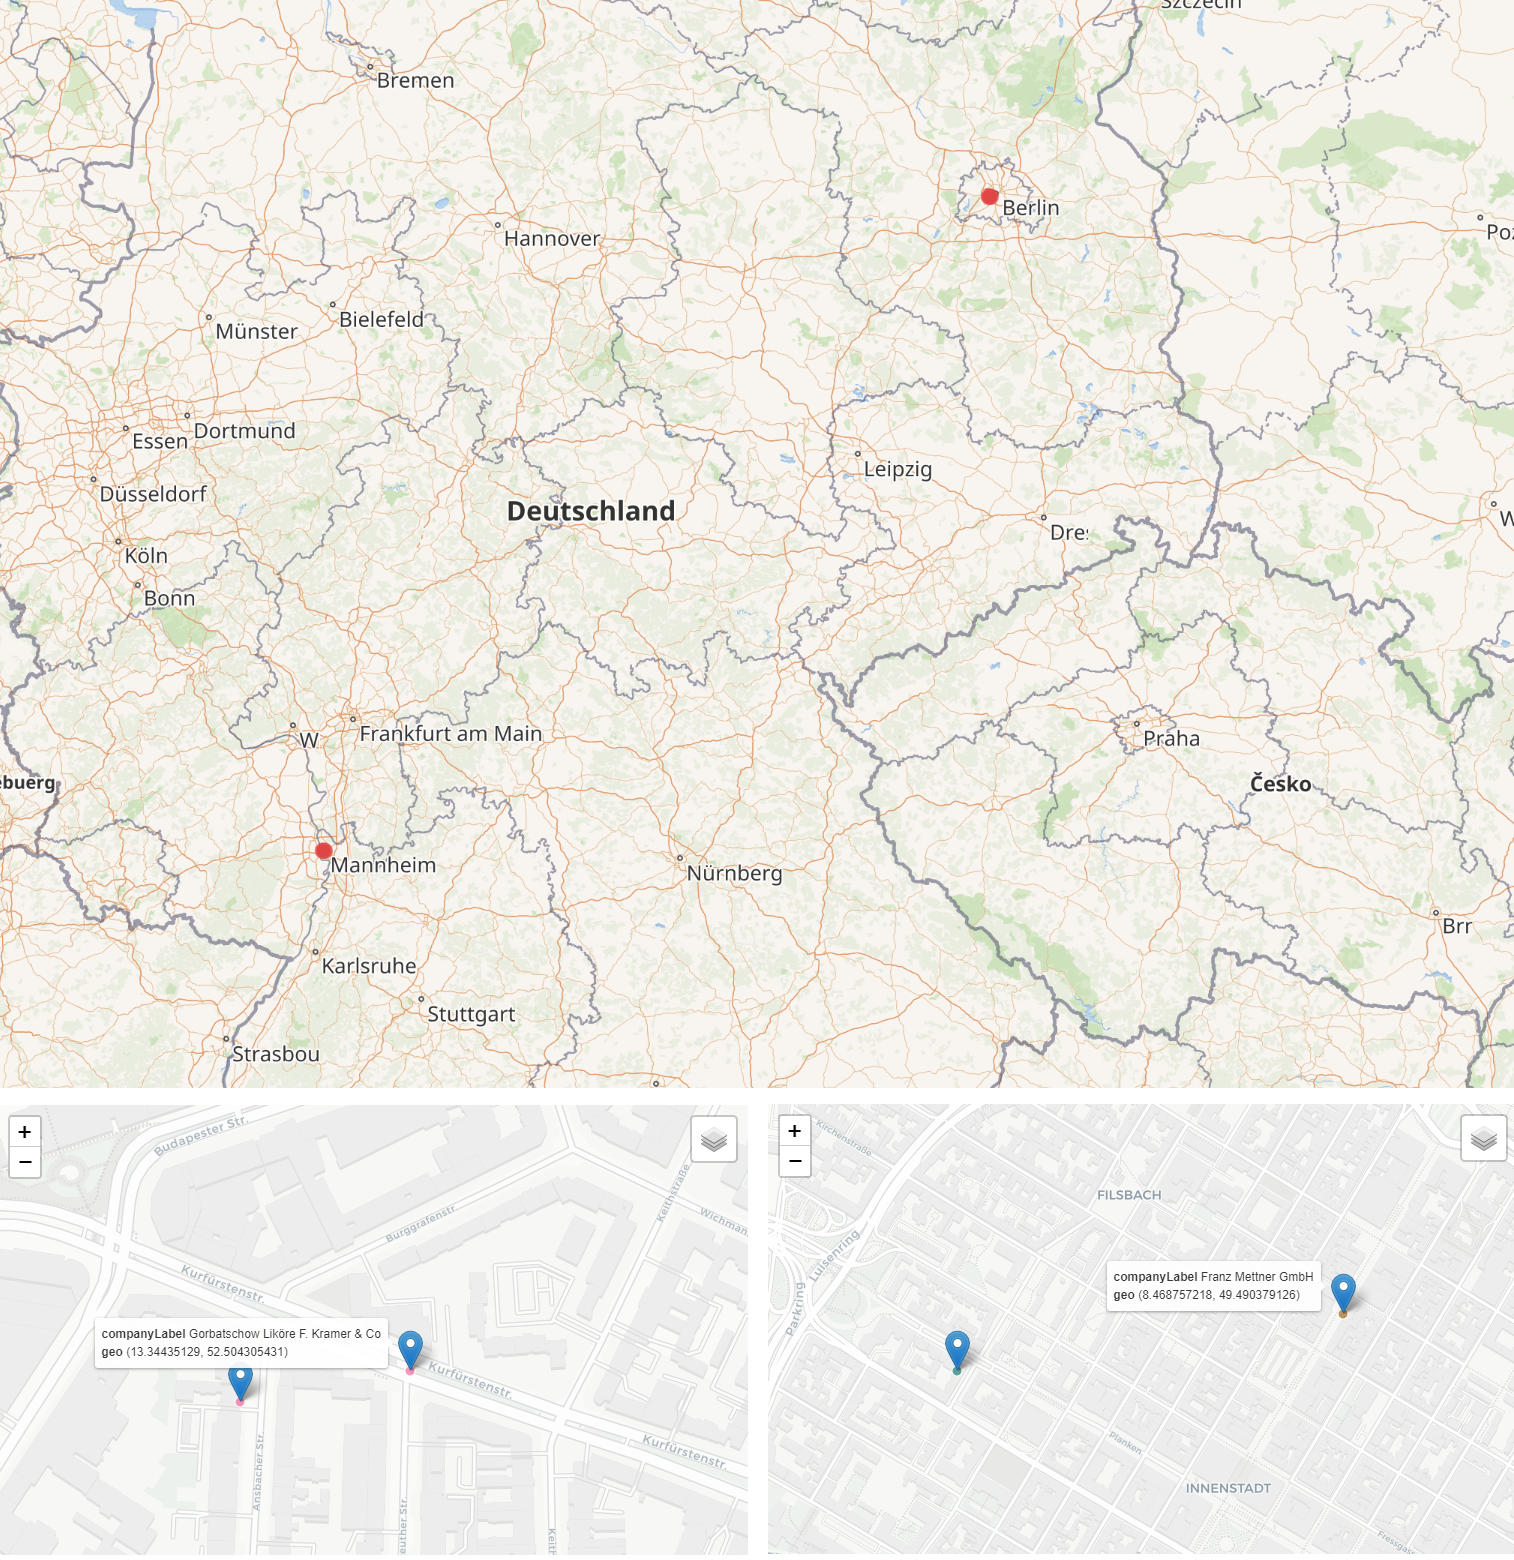
\includegraphics[width=\ScaleIfNeeded]{wikidata-map}}
    \caption{Kartenvisualisierung der Standorte der Jüdischen Gewerbebetriebe, oben direkt im Query Service mit OpenStreetMap (OSM) als Kartendienst, unten in ,,Wikidata Visualization'' mit CartoDB. Unten links Berlin: die gleichfarbigen Punkte markieren Standorte des selben Gewerbebetriebs. Unten rechts Mannheim: verschiedenfarbige Punkte markieren unterschiedliche Gewerbebetriebe.}
    \label{fig:x cubed graph}
\end{figure}

\paragraph{Geschäftsfrauen}
Bislang spielte es in den Lokalstudien noch gar keine Rolle, ob es sich bei den Eigentümern von Jüdischen Gewerbebetrieben um Frauen oder Männer gehandelt hatte. Da nur die Vor- und Nachnamen erfasst wurden, sind geschlechterspezifische Fragestellungen bisher statistisch auch nicht greifbar. Dabei wäre durchaus interessant, welchen Anteil Frauen am Gewerbeleben hatten, in welchen Branchen sie vorwiegend selbstständig tätig waren und ob sie andere Abwehrstrategien verfolgten als männliche Eigentümer. Fakt ist, dass hierfür eine Gender-Angabe in den Daten notwendig ist, die in Wikidata jedoch schon vorhanden ist und nachgenutzt werden kann. Damit ließen sich perpektivisch Datenabfragen zum Geschlechterverhältnis entwickeln (Abbildung 4.21). 

\begin{figure}[h]
    \centering
    \frame{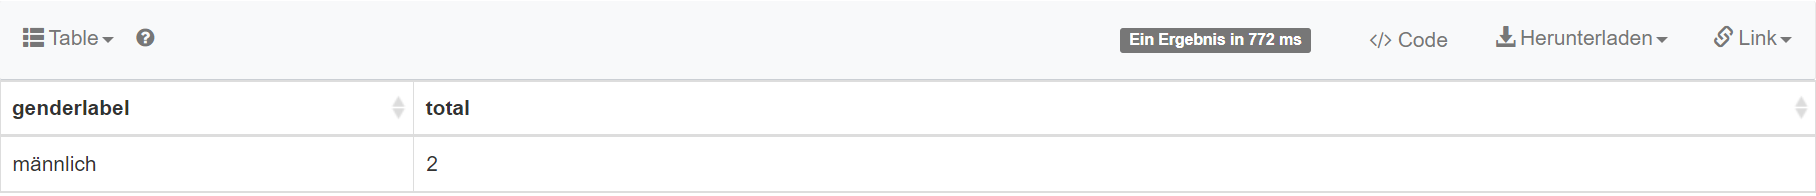
\includegraphics[width=\ScaleIfNeeded]{wikidata-sparql-gender}}
    \caption{Geschlechterverhältnis der Eigentümer Jüdischer Gewerbebetriebe.}
    \label{fig:x cubed graph}
\end{figure}

\subsection{Vernichtung}

Den größten Teil bei der statistischen Analyse nahm der Prozess der Vernichtung der jüdischen Gewerbetätigkeit ein. Dieser bestand, wie in Kapitel 3.1 erläutert wurde, wiederum aus den beiden Teilprozessen Besitzübernahme und/ oder Liquidation. Statistisch lässt sich die Prozesshaftigkeit der Vernichtung schwer greifen, daher wurden für die Studien zu Berlin und Frankfurt a.M. signifikante punktuelle Daten als Analyseeinheiten herausgearbeitet, mit denen sich der Prozess annähernd untersuchen ließ. Diese sind zusammengefasst:

\begin{itemize}
    \item Datum mit mind. Monat und Jahr der gewerblichen Abmeldung.
    \item Datum mit mind. Monat und Jahr der Einleitung des Liquidationsvorgangs (durch einbestellten Liquidator oder von Amts wegen).
    \item Datum mit mind. Monat und Jahr der Löschung.
\end{itemize}

Da in den anderen Forschungsdaten oft nur Jahresangabe zu den beiden Prozessen vorhanden sind, ist nicht klar, auf welches Ereignis diese rekurrieren (Abbildung 4.22).   

\begin{figure}[h]
    \centering
    \frame{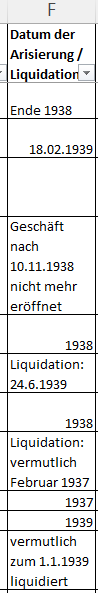
\includegraphics[scale=0.6]{date-vernichtung}}
    \caption{Jahresangaben zu Liquidationen/ Besitzübernahmen.}
    \label{fig:x cubed graph}
\end{figure}

Wikidata hat zum Konzept ,,Zeit/ Datum'' bereits viele Optionen. Demnach wäre der Vorschlag, die reinen Jahresangaben als Intervall zu verstehen und diese statt mit ,,zum Zeitpunkt/ Stand'' (P585) mit ,,betroffener Zeitraum'' (P1264) im Datenobjekt anzureichern (Qualifier). Dies würde die Prozesshaftigkeit von Besitzübernahme und Liquidation deutlich machen. Sofern es konkrete Ereignisse mit Datum gibt, können sie als weitere Qualifier wie oben ergänzt werden. Auf diese Weise ließen sich die unterschiedlichen Forschungsdaten vereinheitlichen und deren Aussagegehalt durch Wikidata sogar noch verfeinern. Der Vorteil von vollständigen Datumsangaben ist, dass sich damit Zeitreihen-Analysen in Wikidata durchführen lassen, die bei reinen Jahresangaben verfälscht werden, da hier automatisch der 01. Januar als Startzeitpunkt gesetzt wird. 


\subsection{Abwehrstrategien}
\paragraph{Umzüge}

über Personen, Normdaten zu Personen, darüber werden die Umzüge greifbar


SPARQL voraussetungsreich muss beherrscht werden, Queries die sich für jede Studie immer wiederholen, können zur Vereinfachung und Hilfestellung die Queries im Wikidata projekt dokuemntiert werden, sodass sie von jedem nachgenutz und angepast werdne können. auf diese weise wir dauch sicher gestellt, dass identische abfragen verwendet werden und Risikp der Dtenverfäslchung durch falsche queris minimiet, wenn jeder einzeln für scih entiwct
  
\section{Veröffentlichung und Nachnutzung}

Wikidata in der offenen Lizenz, die es gibt nämlich jede Nutze ohne Namensnennung
Fraglich, inwiefern das zumindest im akademischen Bereich funktioniert, wo Zitation essentiell für Reputations sind.
Für Regierungsdaten in Deutschland wurde die ,,Datenlizenz Deutschland'' entwickelt die zwei Varianten hat
Namensnennung
Zero 
von  

Vorteil: Daten können ergänzt werden, auch zu den bestehenden fehlen noch Informationen --> hier Mannheim und ZHRB

Methodenübertragbeitkeit nicht im großen Stil aber verinzelt

Datenpräsentation möglich --> Portal wie Archivführer bauen 

Daten können aber auch in gänzlich anderen Kontexten verwenden, die heute noch gar nicht antizpiert werdne


\paragraph{Teamarbeit}
bei der Erfassung und nachträglichen Bearbeitung von Daten (vor allem Anreicherung von Quellendaten)
Sowohl Datenfelder als auch Eingabe

aber auch in Hinblick auch Partizipationsgedanke wurde hier mit aufgegriffen, der in Kapitel 3.2.3 bereits als Kriterium von offenem FDM festgelegt wurde, findet sich auch in den Interviews wieder. Alle grundsätzlich positiv gegenüber Citizen Science eingestellt und sehen es nicht als Behinderung für die wissenschaftliche Forschung 

Strategieentwicklung

\paragraph{Diskussionsforum}
bringt Kollaboration mit sich, dass Diskurs ermöglicht wird, wo Regeln vereinbart werden können, verständigt sich auf Vokabular, Normdaten etc., Weiterentwicklung des Datenmodells
\paragraph{Dynamische Anpassungen}
Flexible und stetige 
Dateneditierebene als auch auf Datenmodellebene
Datenmodell steht nicht von Anfang fest, sondern ist dynamisch, hängt mit den Erhebungsmethoden zusammen
\paragraph{Multiperspektivischer Datenzugang}
Heusler

\paragraph{Datentransfer und Nachnutzung}
Recherche in Datensammlungen
Daten für Erinnerungsinitiativen zur Verfügung stellen, verschiedene Visualisierungmöglichkeiten

\paragraph{Dauerhafte Kuratierung und -pflege}
keine tote Daten produzieren

\paragraph{Test- und Evaluationsphasen}
der Forschungsdatenumgebung, Mitsprache bei neuen Funktionalitäten, Involvierung in den Entwicklungsprozess

\section{Archivierung}
Möglichkeiten des Datenexports in Wikidata --> kann in Zenodo hochgeladen werden, dort mit doi versehen werden

\singlespacing 
\chapter{Diskussion und Empfehlungen}
Wie kann Schnittstelle zwischen Wissenschaft und öffentlichem Wissen/ Öffentlichkeit funktionieren (Fellow-Programm Wikimedia)

hier auf Desiderate aus den Interviews eingehen

\paragraph{Benefits}

\paragraph{Drawbacks}

Datenqualität in Wikidata nicht perfekt, aber bei Christoph auch nicht
Datenkonsistenz und -integrität

\paragraph{Sideeffects}

Datenqualität der Wikidata verbessern und Informationen auf der Wikipedia nachweislich stärker kontextualisieren als bisher
--> am Beispiel von \url{https://de.wikipedia.org/w/index.php?title=Wodka_Gorbatschow&oldid=222273519} und Q2587685

Abschließend zur Forschungsfeldbetrachtung ist festzustellen, dass das dieses inhaltlich mit steigender Anzahl von Lokalstudien in den letzten 20 Jahren enorm voranschritt, aber im Vergleich auf konzeptueller Ebene die Weiterentwicklung überraschend stagnierte. Wenn mehrheitlich in den Studien der Begriff ,,Arisierung'' (oder ,,Entjudung'') kritisch und problemorientiert hinterfragt wird, in der Konsequenz aber nicht aus der wissenschaftlichen Arbeit verbannt, sondern entgegen der eigenen Argumentation als Untersuchungsbegriff beibehalten wird, dann herrscht ein offensichtlicher Mangel an einer breiteren konzeptionellen und methodischen Auseinandersetzung im Forschungsfeld. Dafür spricht auch, dass es bis heute keine einheitliche Definition des Begriffs gibt.\footnote{Und die es auch in der Geschichte des Begriffs nie gegeben hat.\textbf{Vgl. Nietzel und Kreutzmüller}} Einerseits wird darunter speziell der Transfer von jüdischem Eigentum, insbesondere Firmeneigentum, in nicht-jüdischen Besitz und andererseits generisch der gesamte Prozess der wirtschaftlichen Existenzvernichtung der Juden gefasst, wobei dieser unterschiedlich ausgedehnt wurde\footnote{Nachweis} Einen allgemeingültigen wissenschaftlichen Konsens scheint es auf der methodischen Ebene im Forschungsfeld nicht zu geben. Unklar ist, warum nach den eindeutig nachvollziehbaren Gegeneinwänden und alternativen Vorschlägen aus dem Forschungsfeld selbst sich diese methodische Schwäche bis heute hartnäckig hält.


Die Herausforderung besteht darin, zentrale sowie einheitliche Infrastrukturen zu schaffen, die von den überwiegend einzelgeförderten Forschungsprojekten - bei der DFG immerhin mehr als ein Drittel im Jahr 2020 projektbezogener Einzelförderung – nicht allen Forschungsvorhaben ein nachhaltiges Forschungsdatenmanagement inhärent ist. Da es entsprechende Forschungsgebiete in der Vergangenheit schlichtweg noch nicht gab, war der Umgang mit Forschungsdaten mehr von individuellen digitalen Kenntnissen und Kompetenzen des oder der Wissenschaftler*in abhängig als von allgemeingültigen wissenschaftlichen Kriterien sowie technischen Standards. Zeitökonomisch betrachtet bedeutet der wissenschaftliche Umgang mit digitalen Forschungsdaten zudem Arbeitsaufwand, der zu den routinierten Abläufen hinzukommt. Erst recht, wenn sich ganz neu mit dieser Thematik auseinandergesetzt werden muss. Das wirft die berechtigte Frage nach dem Kosten-Nutzen-Verhältnis für die eigene Forschungsarbeit auf.

Eine Synthese dieser bisher nebeneinander existierenden Forschungsergebnisse gibt es noch nicht.\footnote{Vgl. Nietzel S.}

\singlespacing 
\chapter{Fazit und Ausblick}
\onehalfspacing



Drei wesentliche Erkenntnisse:

1. Interviews haben gezeigt, dass Bedarfe adhoc nicht eindeutig formuliert werden (können), was aber nicht bedeutet, dass diese nicht vorhanden sind oder das Wissenschaftler diese nicht sehen (es braucht Übersetzungszeit) sondern unterschiedliche Sprachwelten aufeinander prallen, Kommunikation essenziell --> hier braucht es Übersetzer, wie es mit dieser Masterarbeit unternommen wurde. Erkenntnis, die persönlich aus dieser Arbeit mitgenommen wird, dass Fragen teilweise viel zu technisch gestellt waren, würde heute anders gestellt werden, d.h. Versuch der Übersetzungen, Bedarfsformulierung scheitert nicht an mangelnden Bedarfen sondern wegen der Kommunikation

2. Gerade für verteilte projektbasierte Forschungsvorhaben zu einem Themenkomplex wie der Vernichtung der wirtschaftlichen Existenz sind zentralere Services notwendig, Projekte institutionell unterschiedlich angebunden, welche jeweils ihre eigenen Dienste und Infrastrukturen haben. Für das Forschungsfeld kann es konzeptionell ein immenser Fortschritt bedeuten, projektübergreifend kollaborativ zu arbeiten. Reichen Datenrepositorien Fortschritt, wären aber für das Forschungsfeld nicht ausreichend, braucht auf der Ebene der Datenmodellierung Infrastrukturen

3. Forschung ist nicht auf die akademische Wissenschaft allein beschränkt wie das hier betrachtete Forschungsfeld besondern deutlich macht, die Frage ist, wie bekommt man die unterschiedlichen Akteure zusammen bzw. welche Akteure werden einbezogen und welche ausgeschlossen

4. Wenn entsprechende Infrastrukturen vorhanden und genutzt werden, das zeigt die prototypische Implementierung, Open Science erweitert Erkenntnismöglichkeiten, welche im Ergebnis zu einem Erkenntnisfortschritt führen können. Verschiebt Erkenntnisgrenzen


Denn was Open Science am Ende ist, ist - wenn man der Open-Bewegung konsequent folgt - keine Frage von einzelnen Akteuren, sondern ein andauernder demokratischer Aushandlungsprozess vor allem aber nicht ausschließlich auf der wissenschaftlichen Ebene

\singlespacing 
\appendix
\chapter{Literatur}
\onehalfspacing
\printbibliography[
    heading=bibintoc,
    title={Literaturverzeichnis}
    ]
\chapter{Abbildungsverzeichnis}

\chapter{Forschungsdaten}
\section{Transkripte}
\section{Codesystem}
\section{Modellierungen}
\section{SPARQL-Beispielabfragen}

\end{document}

